% Version 0; Rough outline by SH
% Version 1; First draft by SH
% Version 2; Finish main text; with edits from Susan Foster
% Version 3; More edits from Susan
% Version 4; Edits from Alexie

%% ------------------------------------------------------------------------------------ %%
\documentclass[useamsfonts]{pasj01}
\twocolumn

%% ------------------------------------------------------------------------------------ %%
% Packages
\usepackage{url}
\usepackage{natbib}
\usepackage{latexsym}
\usepackage{morefloats}
\usepackage{xspace}
\usepackage[usenames, dvipsnames]{xcolor}

%% ------------------------------------------------------------------------------------ %%

% Figure extension
\DeclareGraphicsExtensions{.pdf,.png,.eps}

%%%%%%%%%%%%: User Defined Commands %%%%%%%%%%%%

%% ------------------------------------------------------------------------------------ %%
% Song Huang's definition
\def\arcsec{{\prime\prime}}
\def\arcmin{{\prime}}
\def\degree{{\circ}}
\def\h{\hskip -3 mm}
\def\amin{$^\prime$}
\def\asec{$^{\prime\prime}$}
\def\deg{$^{\circ}$}
\def\ddeg{{\rlap.}$^{\circ}$}
\def\dsec{{\rlap.}$^{\prime\prime}$}
\def\lax{{$\mathrel{\hbox{\rlap{\hbox{\lower4pt\hbox{$\sim$}}}\hbox{$<$}}}$}}
\def\gax{{$\mathrel{\hbox{\rlap{\hbox{\lower4pt\hbox{$\sim$}}}\hbox{$>$}}}$}}
\def\simlt{\lower.5ex\hbox{$\; \buildrel < \over \sim \;$}}
\def\simgt{\lower.5ex\hbox{$\; \buildrel > \over \sim \;$}}
\def\micron{{$\mu$m}}
\def\perang{\AA$^{-1}$}
\def\peryr{yr$^{-1}$}
\def\sb{mag~arcsec$^{-2}$}
\def\lsun{$L_\odot$}
\def\msun{$M_\odot$}
\def\sigs{$\sigma_*$}

\def\etal{{\ et al.~}}
\def\galfit{{\tt GALFIT}}
\def\ser{{S\'{e}rsic\ }}

\def\logms{{$\log (M_{\star}/M_{\odot})$}~}
\def\mstar{{$M_{\star}$}~}
\def\logmh{{$\log (M_{\mathrm{halo}}/M_{\odot})$}~}
\def\m2l{{$M_{\star}/L_{\star}$}~}

\newcommand{\alexie}[1]{\textcolor{blue}{\textbf{[Alexie: #1]}}}

\def\redm{\texttt{redMaPPer}}
\def\hscpipe{\texttt{hscPipe}}
\def\synpipe{\texttt{SynPipe}}
\def\cmodel{\texttt{cModel}}
\def\forced{\texttt{forced}}
\def\coadd{\texttt{coadd}}
\def\unforced{\texttt{unforced}}
\def\tract{\texttt{Tract}}
\def\visit{\texttt{Visit}}
\def\tracts{\texttt{Tracts}}
\def\visits{\texttt{Visits}}
\def\galsim{\texttt{G}{\scriptsize \texttt{AL}}\texttt{S}{\scriptsize \texttt{IM}}}
\def\hst{{\textit{HST}}}
\def\s2n{{$\mathrm{S}/\mathrm{N}$}}

%% ------------------------------------------------------------------------------------ %%

% Commenting:
%% ------------------------------------------------------------------------------------ %%
\newcommand{\plan}[1]{\textcolor{blue} {\textbf{#1}}}
\newcommand{\todo}[1]{\textcolor{red} {\textbf{#1}}}
\newcommand{\song}[1]{\textcolor{cyan} {\textbf{#1}}}
\newcommand{\addref}{{\textcolor{red}{\textbf{REF}}}}
\newcommand{\term}[1]{\textbf{\texttt{#1}}}
\newcommand{\susan}[1]{\textcolor{magenta} {\textbf{#1}}}

\newcommand{\plus}{\raisebox{.4\height}{\scalebox{.6}{+}}}
\newcommand{\minus}{\raisebox{.4\height}{\scalebox{.8}{-}}}

%%%%%%%%%%%%: Header and Version %%%%%%%%%%%%

%% ------------------------------------------------------------------------------------ %%

\begin{document}

\SetRunningHead{Huang et al.}{HSC-SSP SynPipe}

\Received{$\langle$April 2017$\rangle$}
\Accepted{$\langle$2017$\rangle$}
\Published{$\langle$2017$\rangle$}

%%%%%%%%%%%%: Title and Affiliations %%%%%%%%%%%%

%% ------------------------------------------------------------------------------------ %%
\title{Characterization and Photometric Performance of the Hyper Suprime-Cam Software Pipeline.}

\author{Song Huang \altaffilmark{1,2}
        Alexie Leauthaud \altaffilmark{1,2},
        Ryoma Murata \altaffilmark{2, 4},
        Jim Bosch \altaffilmark{3},
        Paul Price \altaffilmark{3},
        Robert Lupton \altaffilmark{3},
        Rachel Mandelbaum \altaffilmark{5},
        Claire Lackner \altaffilmark{2},
        Steven Bickerton \altaffilmark{2},
        Satoshi Miyazaki \altaffilmark{6}, 
        Jean Coupon \altaffilmark{7},
        HSC Collaboration \altaffilmark{8}}
%% ------------------------------------------------------------------------------------ %%

\altaffiltext{1}{Department of Astronomy and Astrophysics, University of California,
    Santa Cruz, 1156 High Street, Santa Cruz, CA 95064 USA}
    
\altaffiltext{2}{Kavli Institute for the Physics and Mathematics of the
    Universe, The University of Tokyo Institutes for Advanced Study,
    the University of Tokyo (Kavli IPMU, WPI), Kashiwa 277--8583, Japan}

\altaffiltext{3}{Department of Astrophysical Sciences, Princeton University,
    4 Ivy Lane, Princeton, NJ 08544}

\altaffiltext{4}{Department of Physics, University of Tokyo, Tokyo 113-0033, Japan}

\altaffiltext{5}{McWilliams Center for Cosmology, Department of Physics,
    Carnegie Mellon University, Pittsburgh, PA 15213, USA}

\altaffiltext{6}{SOKENDAI (The Graduate University for Advanced Studies), Mitaka,
    Tokyo, 181--8588, Japan}

\altaffiltext{7}{Department of Astronomy, University of Geneva, ch. d'\'Ecogia 16, 
    1290 Versoix, Switzerland}

\altaffiltext{8}{Other affiliations}

\email{song.huang@ipmu.jp}
%% ------------------------------------------------------------------------------------ %%

%%%%%%%%%%%%: Abstract and Keywords %%%%%%%%%%%%

%% ------------------------------------------------------------------------------------ %%
\KeyWords{Surveys,
          Methods: observational,
          Techniques: photometric}

\maketitle

%% ------------------------------------------------------------------------------------ %%
\begin{abstract}

    The Subaru Strategic Program (SSP) is an ambitious wide-area, multi-band survey
    using the Hyper Suprime-Cam (HSC) on the Subaru telescope. The  Wide layer of the SSP is both wide and deep, reaching a detection limit of $i>26.0$ mag. At these depths, it is challenging to achieve accurate, unbiased, and consistent photometry across all
    five bands. The HSC data are reduced using a pipeline that builds on the prototype pipeline being designed by the Large Synoptic Survey Telescope’s Data Management system. We have developed a \texttt{Python}-based, flexible framework to inject synthetic galaxies into real HSC images called \synpipe{}. In this paper, we explain the design and implementation of \synpipe{} and we generate a sample of synthetic galaxies to examine the photometric performance of the HSC pipeline. For stars, we achieve 1\% photometry at $i{\sim}18.0$ mag and 7\% photometry at $i{\sim}25.5$ in the $i$-band (corresponding to uncertainties of ${\sim}0.01$ and ${\sim}0.06$ mag respectively). \alexie{Put numbers in here using this phrase format} For synthetic galaxies with single-\ser{} profiles, forced \cmodel{} photometry achieves 1\% photometry at $i{\sim}18.0$ mag and 7\% photometry at $i{\sim}25.5$ in the $i$-band (corresponding to uncertainties of ${\sim}0.01$ and ${\sim}0.06$ mag respectively). 
    %For synthetic galaxies based on a single-\ser{} model, uncertainties of the
    %forced \cmodel{} photometry typically range from 0.14 mag at $i{\sim}20.0$ mag
    %to 0.20 mag at $i{\sim} 25.2$ mag.
    we show that
    both \forced{} PSF and \cmodel{} photometry yield unbiased color estimates
    that are robust to seeing conditions. We identify several caveats that apply to version xxx of the  HSC pipeline and than need to be considered when using data from the first public HSC data release. First, the degree to which an object is blended with other objects impacts the overall photometric performance.  This is especially true for point sources \alexie{quanityf here}. Highly blended objects tend to have larger photometric uncertainties, systematically underestimated fluxes \alexie{Should be overestimated here no?}, and slightly biased colors. Second, a relatively high fraction of faint stars (${\sim}16$\% at $i>22.5$ mag) can be
    misclassified as extended objects \alexie{need to quantify here}. Third, the shape and size estimates for galaxies using \cmodel{} suffer from strong
    biases \alexie{quantify here}.

\end{abstract}
%% ------------------------------------------------------------------------------------ %%

%%%%%%%%%%%%: Main Text %%%%%%%%%%%%

%% ------------------------------------------------------------------------------------ %%
\section{Introduction}
    \label{sec:intro}

    %% Background
    Wide-field, multi-band imaging surveys have stepped onto the central stage of
    modern astrophysics and cosmology over the past decade.  These efforts will soon be replaced with even more ambitious programs such as the Large Synoptic Survey Telescope
    (LSST)\footnote{\url{https://www.lsst.org/}}, the Wide-Field Infrared Survey
    Telescope
    (WFIRST; \citealt{Dressler2012})\footnote{\url{https://wfirst.gsfc.nasa.gov/}},
    and the \textit{Euclid} project
    (\citealt{Laureijs2012})\footnote{\url{http://sci.esa.int/euclid/}}. Among many ongoing efforts, the Subaru Strategic Program
    (SSP; \citealt{HSCDR1})\footnote{\url{http://hsc.mtk.nao.ac.jp/ssp/}}, which
    uses the Hyper Suprime-Cam (HSC; \citealt{Miyazaki2012}) on the prime focus of
    the Subaru telescope, is the most efficient in terms of
    etendue\footnote{The collecting area multiplied by the field of view.}. Surveys such as HSC, and other to follow, will  provide stringent constraints on  the cosmological model,  characterize the evolution of galaxies, map out the stellar structure of our Milky Way, and are poised to discover a large number of interesting transient objects.

    %% Challenges
    Before we can tackle outstanding scientific questions, we must first learn
    how to handle the the large amounts of data\footnote{Right now, SSP has accumulated
    ${\sim}300$ TB of data products.} generated by these projects while satisfying  strict requirements for  high quality image processing with accurate measurement for the magnitudes and shapes of stars and galaxies. Data handling becomes increasingly challenging in the age of modern imaging
    surveys am we aim to characterize and account for subtle effects related to charge-coupled devices (CCDs). Cameras are made up of multiple CCDs, each with slightly different
    characteristics, and have large fields-of-views (FoV) over focal planes that are not perfectly flat. During observations, the seeing and background conditions display spatial and temporal variations across the FoV. The full-depletion, thick CCDs selected for HSC enable long exposure
    times and have excellent red-sensitivity, but they also suffer from the
    so-called ``brighter-fatter'' effect (\citealt{Antilogus2014}), which means that
    brighter stars have larger Point Spread Functions (PSFs) than fainter stars. These variations and effects make accurate astrometric and photometric calibration,
    background subtraction, and point spread function (PSF) modeling intrinsically
    difficult (e.g., \citealt{Schlafly2012}). Furthermore, as surveys reach to increasingly deeper detection limits
    (e.g., the SSP Wide layer reaches a $5\ \sigma$ point source detection limit of
    ${\sim}26.4$ mag), the number of objects per unit area increases.  Hence, deep surveys become  more sensitive and subject to the effects of blending.  The challenge of modern imaging surveys call for  photometric measurement methods
    that are more powerful and precise than those used in previous, shallower surveys.
    
    %
    
    
    These challenges are not merely technical details; their resolution is crucial
    to achieving key scientific goals.
    For instance, weak gravitational lensing (WL; \citealt{Kaiser1993, Bartelmann2001})
    is a powerful tool for measuring the large-scale distribution of dark matter.
    However, WL measurements critically depend on our ability to measure the shape and photometric redshifts of background galaxies with high precision. Photometric redshifts (e.g., \citealt{Benitez2000, Bolzonella2000,
    Ilbert2009}) are fundamentally important for studying the evolution of galaxies,
    and the ``drop-out'' method is critical for selecting high-redshift galaxies
    (e.g., \citealt{Steidel1996}).
    However, both of those methods reply on the availability of accurate multi-band photometric
    measurements. With increasingly large surveys,  and with more stringent requirements on data quality,  quality control also becomes a pressing issue. 
    
   In this paper, we present a \texttt{Python}-based software package called  \synpipe{} that  injects synthetic objects into  HSC images  and  which interfaces with the HSC data reduction pipeline (\hscpipe{}). Among other applications, \synpipe{} can be used to perform quality control and to characterize the performance and limitations of  \hscpipe{}. Several tools with similar goals have been developed (e.g., \citealt{Chang2015,
    Suchyta2016}) for the Dark Energy Survey (DES; \citealt{DES2005}).


 \alexie{Edit here following this format}. In Section 1 we ... in section 2 we ....
    
    Below, we briefly introduce the HSC survey and the current status of data
    reduction (Section \ref{sec:ssp}), explain \synpipe{} design and implementation
    (Section \ref{sec:synpipe}), and demonstrate \synpipe{} usage via straightforward
    tests (Section \ref{sec:test}) that focus on the general photometric quality for
    both synthetic stars and galaxies (Section \ref{sec:result}).
    We then summarize the work and discuss future developments in
    Section \ref{sec:summary}.

    The code for \synpipe{}, along with documentation and examples, is made available
    on GitHub at: \texttt{https://github.com/dr-guangtou/synpipe}.
    
%% ------------------------------------------------------------------------------------ %%

%% ------------------------------------------------------------------------------------ %%
%% Fig: Flowchart
\begin{figure*}
    \begin{center}
        \includegraphics[width=\textwidth]{fig/synpipe_flowchart_new}
    \end{center}
    \caption{
        Illustration of the main steps involved in using \synpipe{}.
        Gray boxes indicate required inputs at different stages.
        The blue box identifies the \texttt{addFakes.py} step, when \synpipe{} injects synthetic objects into single-frame images. Below the blue box, we show an HSC image before and after the insertion of synthetic galaxies. The positions of synthetic  objects are highlighted with green circles. Red boxes depict the image coadding and multi-band measurement steps
        using \texttt{stack.py} and \texttt{multiBand.py}. At the bottom left, we show a \coadd{} image which contains synthetic galaxies. On the right hand side, we show the spatial relation
        between \texttt{Tracts}, \texttt{Patches}, and \texttt{Visits}. The xxxxxxx colored box corresponds to one \texttt{Tract} which has an area of about xx deg$^2$. Large colored circles are \texttt{Visits} (also commonly known as "pointings") with small rectangles representing CCDs. \texttt{Patches} are represented by black dashed lines. One \texttt{Tract} typically contains xx  \texttt{Patches}.}
    \label{fig:flowchart}
\end{figure*}
%% ------------------------------------------------------------------------------------ %%

%% ------------------------------------------------------------------------------------ %%
\section{Hyper-Suprime Cam Subaru Strategic Program (HSC Survey)}
    \label{sec:ssp}

    %% Basic
    Taking advantage of the new prime focus camera on the 8.2--m Subaru telescope,
    the ambitious HSC survey consists of three layers: Wide, Deep, and UltraDeep.
    The Wide layer will map a total of ${\sim}1400$ deg$^2$ of sky in five broad bands
    ($grizy$; Kawanomoto\etal in prep.).
    The Deep (four separated fields; ${\sim}27$ deg$^2$) and UltraDeep (two separated
    fields; ${\sim}3.5$ deg$^2$) layers use a few additional narrow-band filters
    and employ a slightly different surveying strategy.
    Strauss\etal (in prep.) describes the HSC survey in more detail, and identifies the
    HSC collaborators.

    The HSC camera (\citealt{Miyazaki2012}) is made up of 124 full-depletion thick
    CCDs: 112 for science and another 12 for guiding and focusing.
    The camera has a circular FoV with a 1.5 deg diameter.
    Each CCD contains 2048$\times$4096 pixels and the sizes of pixels are 0.168\asec{}.

    In February 2017, the HSC collaboration released the first 1.7 years of data to
    the public (DR1;
    \citealt{HSCDR1})\footnote{\texttt{https://hsc-release.mtk.nao.ac.jp }}.
    For our work, we focused on data from the Wide layer as they relate to key
    scientific goals of the HSC survey, which include weak lensing cosmology, galaxy evolution, and studies of galaxy clusters.  The Wide layer data in DR1 corresponds to ${\sim}108$ deg$^2$ spread over 
   six fields (XMM--LSS, GAMA09H, WIDE12H, GAMA15H, HECTOMAP, and VVDS)
    \footnote{A small AEGIS field is also observed for calibration purposes.}.
    Except for the HECTOMAP field, the regions are all close to the equator.
    In the Wide layer, the $g$ and $r$ bands have 10 minute exposures broken into four
    dithers.  The  $i$, $z$, and $y$ bands have 20 minute exposures broken into six dithers. The survey prioritizes the observations so that the $i$-band has the best seeing conditions to improve galaxy shape measurements for weak lensing science. The  $i$ band data in the Wide layer reach a $5\sigma$ point source limiting magnitude of  $i{\sim} 26.4$ mag  and have a median seeing with FWHM${\sim}0.6$\asec{}. \citealt{HSCDR1} provides details on the first data release and data status.

%% ------------------------------------------------------------------------------------ %%

%% ------------------------------------------------------------------------------------ %%
\section{The HSC Data Reduction Pipeline}
    \label{ssec:hscpipe}

The HSC data are reduced using a pipeline that builds on the prototype pipeline being designed by the Large Synoptic Survey Telescope’s Data Management system (\citealt{Ivezic2008, Axelrod2010,
    Juric2015}) and is described in Bosch\etal (in prep.). DR1 data are reduced by \hscpipe{} \texttt{v4.0.5}. Because\synpipe{} is intrinsically connected to the complex data reduction
    processes in \hscpipe{}, we briefly introduce the main steps below, and we introduce a few key HSC/LSST terms.

    \begin{enumerate}

        \item \textbf{Single-\texttt{Visit~}Processing}:
            Each individual exposure is called a \term{Visit} and is assigned
            an even integer.
            After initial data screening (considering the background level, seeing, and transparency
            Furusawa\etal in prep.), \hscpipe{} detrends these data (subtraction
            of overscan, bias, and dark; flatfielding), \alexie{xxxxx} generates variance and mask
            images, subtracts the background, and provides initial astrometric and
            photometric calibrations. \synpipe{} uses the spatially varying PSF models, photometric zeropoints, and the World Coordinate System (WCS; \citealt{WCS1, WCS2})
            corrected for optical distortion provided by \hscpipe{}.
        \item \textbf{Multi-\visit{} Processing}:
            After single-\visit{} processing, \hscpipe{} warps and mosaics the
            reduced CCD images into much deeper \coadd{} images while improving
            the astrometric and photometric calibrations via processes similar to
            the \"{u}ber-calibration in the Sloan Digital Sky Survey (SDSS)
            \citep{Padmanabhan2008}.
            \textbf{\synpipe{} will use these improved calibrations.}
            \hscpipe{} organizes these \coadd{} images into equiareal rectangular
            regions, or \tracts{}, which are predefined as iso-latitude tessellations.
            One \tract{} covers approximately $1.7\times 1.7$ degrees$^2$ and
            adjacent \tracts{} overlap each other by ${\sim}1$\amin{}.
            Each \tract{} is further divided into $9\times9$ \texttt{Patches}.
            A \texttt{Patch} is a $4200\times4200$ pixels rectangular region, and
            adjacent \texttt{Patches} overlap each other by 100 pixels.   
        \item \textbf{Multi-band Measurements}:
            To achieve consistent photometry across all filters, \hscpipe{} first
            detects and deblends objects on \coadd{} images in each band
            independently (the \unforced{} measurements).
            The collection of above-threshold pixels for each object is referred to as
            a \texttt{footprint}.
            \hscpipe{} merges the \texttt{footprints} and flux peaks in the different
            bands and then selects a reference band for each object based on its $S/N$ in each band (usually this corresponds to the $i$-band).  Centroids, shapes, and other non-amplitude parameters are then fixed to  the values from the reference band. \hscpipe{} then performs \forced{} photometry using these fixed quantities. The goal of the  \forced{} photometry step is to generate accurate colors.
        \item \textbf{HSC Photometry}:
            The multi-band catalogs generated by \hscpipe{} contain various types of photometry measurements (see \citealt{HSCDR1} for details). Here, we focus on characterizing the the \forced{} \texttt{psf} and \cmodel{}
            photometry. The
            \texttt{psf} photometry should provide the most appropriate magnitudes and
            colors for point sources. The  \cmodel{} should be used for galaxies. The HSC  \cmodel{} algorithm is described in Bosch\etal, in prep. and is an  improved version of the SDSS \cmodel{} magnitude (\citealt{Lupton2001, Abazajian2004}). The HSC  \cmodel{} fits objects using both a de Vaucouleurs and an exponential profiles taking into account the smearing by the PSF.  \cmodel{} then linearly combines the two results to find the best fit to the galaxy image. \cmodel{} magnitudes are designed to yield accurate fluxes and colors for galaxies. Star--galaxy separation is performed based on
            the difference between \texttt{psf} and \cmodel{}{} magnitudes.
    \end{enumerate}

    DR1 data quality has been vetted in \citet{HSCDR1} by cross-checking
    with the Panoramic Survey Telescope and Rapid Response System (Pan-STARRS) 1
    imaging survey (\citealt{Schlafly2012, Tonry2012, Magnier2013}) to examine the
    behavior of the stellar sequence.
    Generally speaking, the PSF photometry is accurate at the 1--2\% level \alexie{only for bright stars}, and the
    astrometry is accurate to ${\sim}10$ and 40 max internally and externally.

%% ------------------------------------------------------------------------------------ %%

%% ------------------------------------------------------------------------------------ %%
\section{SynPipe Overview}
    \label{sec:synpipe}

%% ------------------------------------------------------------------------------------ %%
\subsection{Design}
    \label{ssec:design}

    \hscpipe{} is a complex data reduction pipeline that still faces many challenges
    and is under active development.
    Unlike most photometric pipelines on the market, it involves high-level reduction
    processes that produce not only deep \coadd{} images but also a series of
    science-ready catalogs. To perform tests of the  data products that result from \hscpipe{},  \synpipe{} is designed to satisfies a few basic standards:

    \begin{itemize}

        \item \textbf{Realistic Images}:
            Instead of using a fully generative approach to simulate full HSC-like
            images from the ground up (e.g., \citealt{Chang2015}), \synpipe{} injects
            synthetic objects into real HSC images so that all the realistic
            features of the real data (e.g., blended objects; proximity to bright
            objects, bleeding trails, other optical artifacts can be included in the
            test.
            The impact of these features can be important for studies that care about completeness and the selection
            function.
            In \synpipe{}, point sources are simulated using the HSC PSF model,
            and a realistic galaxy model is created by the modular galaxy image
            simulation toolkit, \galsim{} (\citealt{Rowe2015})
            \footnote{\texttt{https://github.com/GalSim-developers/GalSim}}.

        \item \textbf{Authentic Data Processing}:
            To follow the data reduction process as realistically as possible, we choose to
            start from the single-\visit{} images instead of directly putting synthetic
            objects on the final \coadd{} images (e.g., \citealt{Suchyta2016}).
            Through this approach, subtle effects like seeing differences among
            \visits{} and small errors in astrometric calibration can be taken
            into account.
            Every synthetic object will experience all the steps we would use for a real object: detection, deblending, stacking, and measurement.
            This can be important for challenging tasks like WL measurements
            or the detection of high-$z$ galaxies.
            The downside of this choice is that it slows down the overall run-time because we need to inject synthetic objects into all the \visits{} that contribute to a \tract{}.
        \item \textbf{Flexible Capabilities}: \synpipe{} is designed to be flexible enough to be useful for HSC users with a range of scientific goals.
            We provide default catalogs to generate samples of synthetic stars
            and galaxies with realistic magnitudes and color distributions along with
            tools to help the user work on HSC DR1 data. However, \synpipe{} also easily allows users to  design and use their own custom made input catalogs.
            \synpipe{} is already being used in a wide range of
            scientific applications (see Section \ref{sec:summary} for details).

    \end{itemize}
%% ------------------------------------------------------------------------------------ %%

%% ------------------------------------------------------------------------------------ %%
\subsection{\synpipe{} Implementation }
    \label{ssec:flowchart}

    In this section, we describe the \synpipe{} test implementation illustrated in Fig \ref{fig:flowchart}.

%% ------------------------------------------------------------------------------------ %%
\subsubsection{Preparation}
    \label{sssec:prep}

    To create a catalog of synthetic objects, the user first needs to select which HSC data and which input synthetic galaxy catalog to use. 

    \begin{itemize}

        \item \textbf{Information about the data}. This  corresponds to the location of HSC images and a list of \visits{} to be used. \synpipe{} can also help the user identify
            all the \visits{} that contribute to one \tract{} in any given
            band.
            \synpipe{} also provides tools to create an optional bad-pixel mask
            (e.g., bright object, bleeding trails) for a specific \tract{} so that
            the user can avoid putting synthetic objects on problematic regions.

        \item \textbf{Input catalog}. This is a catalog in \texttt{FITS} (Flexible Image Transport System)
            format that contains the  coordinates, magnitudes, and model parameters of synthetic  galaxies.  The positions of synthetic galaxies can be specified  via the input catalog, they can be distributed randomly over a given region, or on a grid (the grid option is useful in that it avoids blends between Synthetic objects, Murata\etal in prep.).  
    \end{itemize}

Synthetic objects can be one of the following:

    \begin{itemize}

        \item \textbf{Point source}: \synpipe{} simply uses the PSF model from \hscpipe{} as the model for
            a point source (stars and/or quasi-stellar objects).
            \hscpipe{} uses a special version of \texttt{PSFEx}
            (\citealt{Bertin2011, Bertin2013}) to characterize PSF as a function
            of position and the PSF model can be reconstructed
            for any location on the image. To inject point sources, the user only needs to specify a catalog of coordinates and magnitudes.
        \item \textbf{\ser{}models}:
            \texttt{SynPipe} uses \galsim{} \texttt{v1.4} (\citealt{Rowe2015}) to
            simulate galaxies.
            \galsim{} is an image simulation tool that was designed for the GRavitational lEnsing Accuracy Testing 3 (GREAT3) challenge
            (\citealt{Mandelbaum2014}). Currently, \synpipe{} allows synthetic galaxies to be modeled by a single
            or a double \citet{Sersic1963}
            profile\footnote{More flexible model choices will be added later.}. The \ser{} profile is flexible enough to describe the overall flux
            distributions of galaxies near and far, both early-type or late-type.
            A double-\ser{} model can simulate a galaxy with even more realistic
            structural details (e.g., bulge$+$disk).
            For each \ser{} component, the user needs to provide the magnitude,
            effective radius ($R_{\mathrm{e}}$, in unit of arcsec), \ser{} index
            ($n_{\mathrm{Ser}}$), axis ratio ($\mathrm{b}/\mathrm{a}$), and position
            angle (PA).
            External shear can also be applied to a synthetic galaxy ($g_1$ and
            $g_2$, see \citealt{Rowe2015} for more details).
        \item \textbf{Galaxies from the GREAT3 challenge}: \synpipe{} also allows users to choose from parametric models or real
            high-resolution galaxy images used in the GREAT3 WL challenge. Real galaxy images are drawn from the \hst{}/ACS F814W ($I$-band) images of galaxies
            in the COSMOS field (e.g., \citealt{Scoville2007,Leauthaud2007}). Instead of using real galaxy images, the users may also use models of  COSMOS galaxies to $I_{\mathrm{Auto}}\leq25.2$ mag via a method developed by
            \citet{Lackner2012}.  Parametric models of COSMOS galaxies include a single-\ser{} and the \ser{}
            bulge$+$Exponential disk model. The parameter values for these models are stored in the
            \texttt{GalSim.COSMOSCatalog()} catalog.
            To access them, the user can provide the ID number of COSMOS galaxies
            in the input catalog, or can simply opt to let \synpipe{} randomly select galaxies from the COSMOS input catalog.
    \end{itemize}
%% ------------------------------------------------------------------------------------ %%

%% ------------------------------------------------------------------------------------ %%
\subsubsection{Injection of Synthetic Objects into Single-\visit{} Images}
    \label{sssec:addFakes}
    
    \alexie{Can we use bullet points to highlight the different steps? This paragraph is really hard to read.}

    With the input catalog and test data information in hand, \synpipe{}injects synthetic
    objects into single-exposure images (step \texttt{addFakes.py}; see the middle panel
    of Fig \ref{fig:flowchart}).
    \synpipe{} goes through all the individual CCD images that belong to each \visit{}
    and decides which synthetic objects from the input catalog need to be injected.
    \synpipe{} uses the \textit{initial astrometric calibration} of each single
    \visit{} to convert the input coordinates into locations on the CCD image. For each synthetic object, \synpipe{} uses the  reconstructed PSF for each exposure.  The photometric zero point from the single-\visit{} calibration is used to convert input magnitudes of synthetic objects into fluxes. For point sources, \synpipe{} generates a rectangular cutout image of the PSF model
    with appropriate size and correct total flux. For galaxies described by single- or double-\ser{} models, \synpipe{} passes the
    input \ser{} index and effective radius to the \galsim{}\texttt{.Sersic} function to
    create a \ser{} component.
    After stretching and rotating the galaxy to the expected axis ratio and position
    angle via the \texttt{shear} and \texttt{rotate} methods, \synpipe{} assigns the
    correct flux to this component.
    For a double-\ser{} model, \synpipe{} uses the \galsim{}\texttt{.Add} method to
    combine two \ser{} components. For  parametric models from the GREAT3 catalog, \synpipe{} uses the
    \texttt{COSMOSCatalog.makeGalaxy} method to generate models.  To inject  real HST galaxy images,  \synpipe{} calls the \galsim{}\texttt{.RealGalaxy} method.
    If necessary, an additional shear ($g_1$ and $g_2$) can be applied to the model at
    this point.
    Then, \synpipe{} passes the reconstructed PSF image into a
    \galsim{}\texttt{InterpolatedImage} object and convolves it with the galaxy model
    using \galsim{}\texttt{.Convolve}.
    After this, \synpipe{} uses the \galsim{}\texttt{.drawImage} method to create the
    image of the simulated galaxy.
    A component with a high \ser{} index ($n_{\mathrm{Ser}} > 4$) often requires a
    large image size to cover all of its flux, so \synpipe{} allows the user to
    truncate the model at a given radius (N$\times R_{\mathrm{e}}$).
    \synpipe{} will also give warning information when a component with $
    n_{\mathrm{Ser}} > 6$ is encountered because it takes much longer to achieve
    accurate PSF convolution in such a model; and the result is, therefore,
    not a realistic galaxy model.

    After \synpipe{} creates the image of the simulated galaxy, it then shifts the
    image according to is location on the CCD on a pixel-by-pixel basis;
    \synpipe{} also crops the images when necessary.
    When that task is complete, \synpipe{} adds appropriate noise to the image based
    on the pixels it covers and the calibration information of the detector, and creates
    a variance image that reflects the influence of the synthetic object.
    Since each HSC CCD consists of 4 amplifiers, each with different characteristics,
    \synpipe{} carefully creates a corresponding gain map to provide accurate noise
    level.
    In the final step, \synpipe{} adds the noise-added image and the variance map to the
    original CCD data while also adding a new \texttt{FAKE} mask bit to the mask plane.
    The middle panel of Fig \ref{fig:flowchart} depicts the result of the
    \texttt{addFakes.py} step by showing an example CCD image before and after the
    synthetic objects are injected.
%% ------------------------------------------------------------------------------------ %%

%% ------------------------------------------------------------------------------------ %%
\subsubsection{Stacking and Multi-band Measurements}
    \label{sssec:multiband}

    The newly generated single-\visit{} images have the same format and data
    structure as real HSC data. To perform stacking and measurements, \synpipe{} calls standard \hscpipe{} routines.
    
    The \texttt{stack.py} step takes the improved astrometric and photometric
    calibrations for each \visit{} from the original reduction and creates
    \coadd{}  images that contain synthetic objects.
    The \texttt{multiBand.py} step then processes these \coadd{}  images and
    provides standard multi-band measurements in FITS catalogs that are grouped by
    \texttt{Patch} ID.

    Using the infrastructures provided by \hscpipe{}, the user can easily perform these steps in parallel, and the overall efficiency of \synpipe{} is similar to
    the real data reduction process. The data and catalog volumes is also similar to the original data reduction process.

 The final step is to identify Synthetic galaxies in the output catalogs. \synpipe{} can match the input catalog to the output catalog (this contains a mix of real and synthetic galaxies) using a matching radius that is specified by the user.
    Each unmatched object from the input catalog is also passed to the results catalog
    with a unique label.
    In the case of multiple matches, the user can choose between returning only the
    closest match or returning all objects within the matching radius (the nearest one
    is labeled as such).
%% ------------------------------------------------------------------------------------ %%

%% ------------------------------------------------------------------------------------ %%
%% Fig: Star Sample
\begin{figure*}
    \begin{center}
        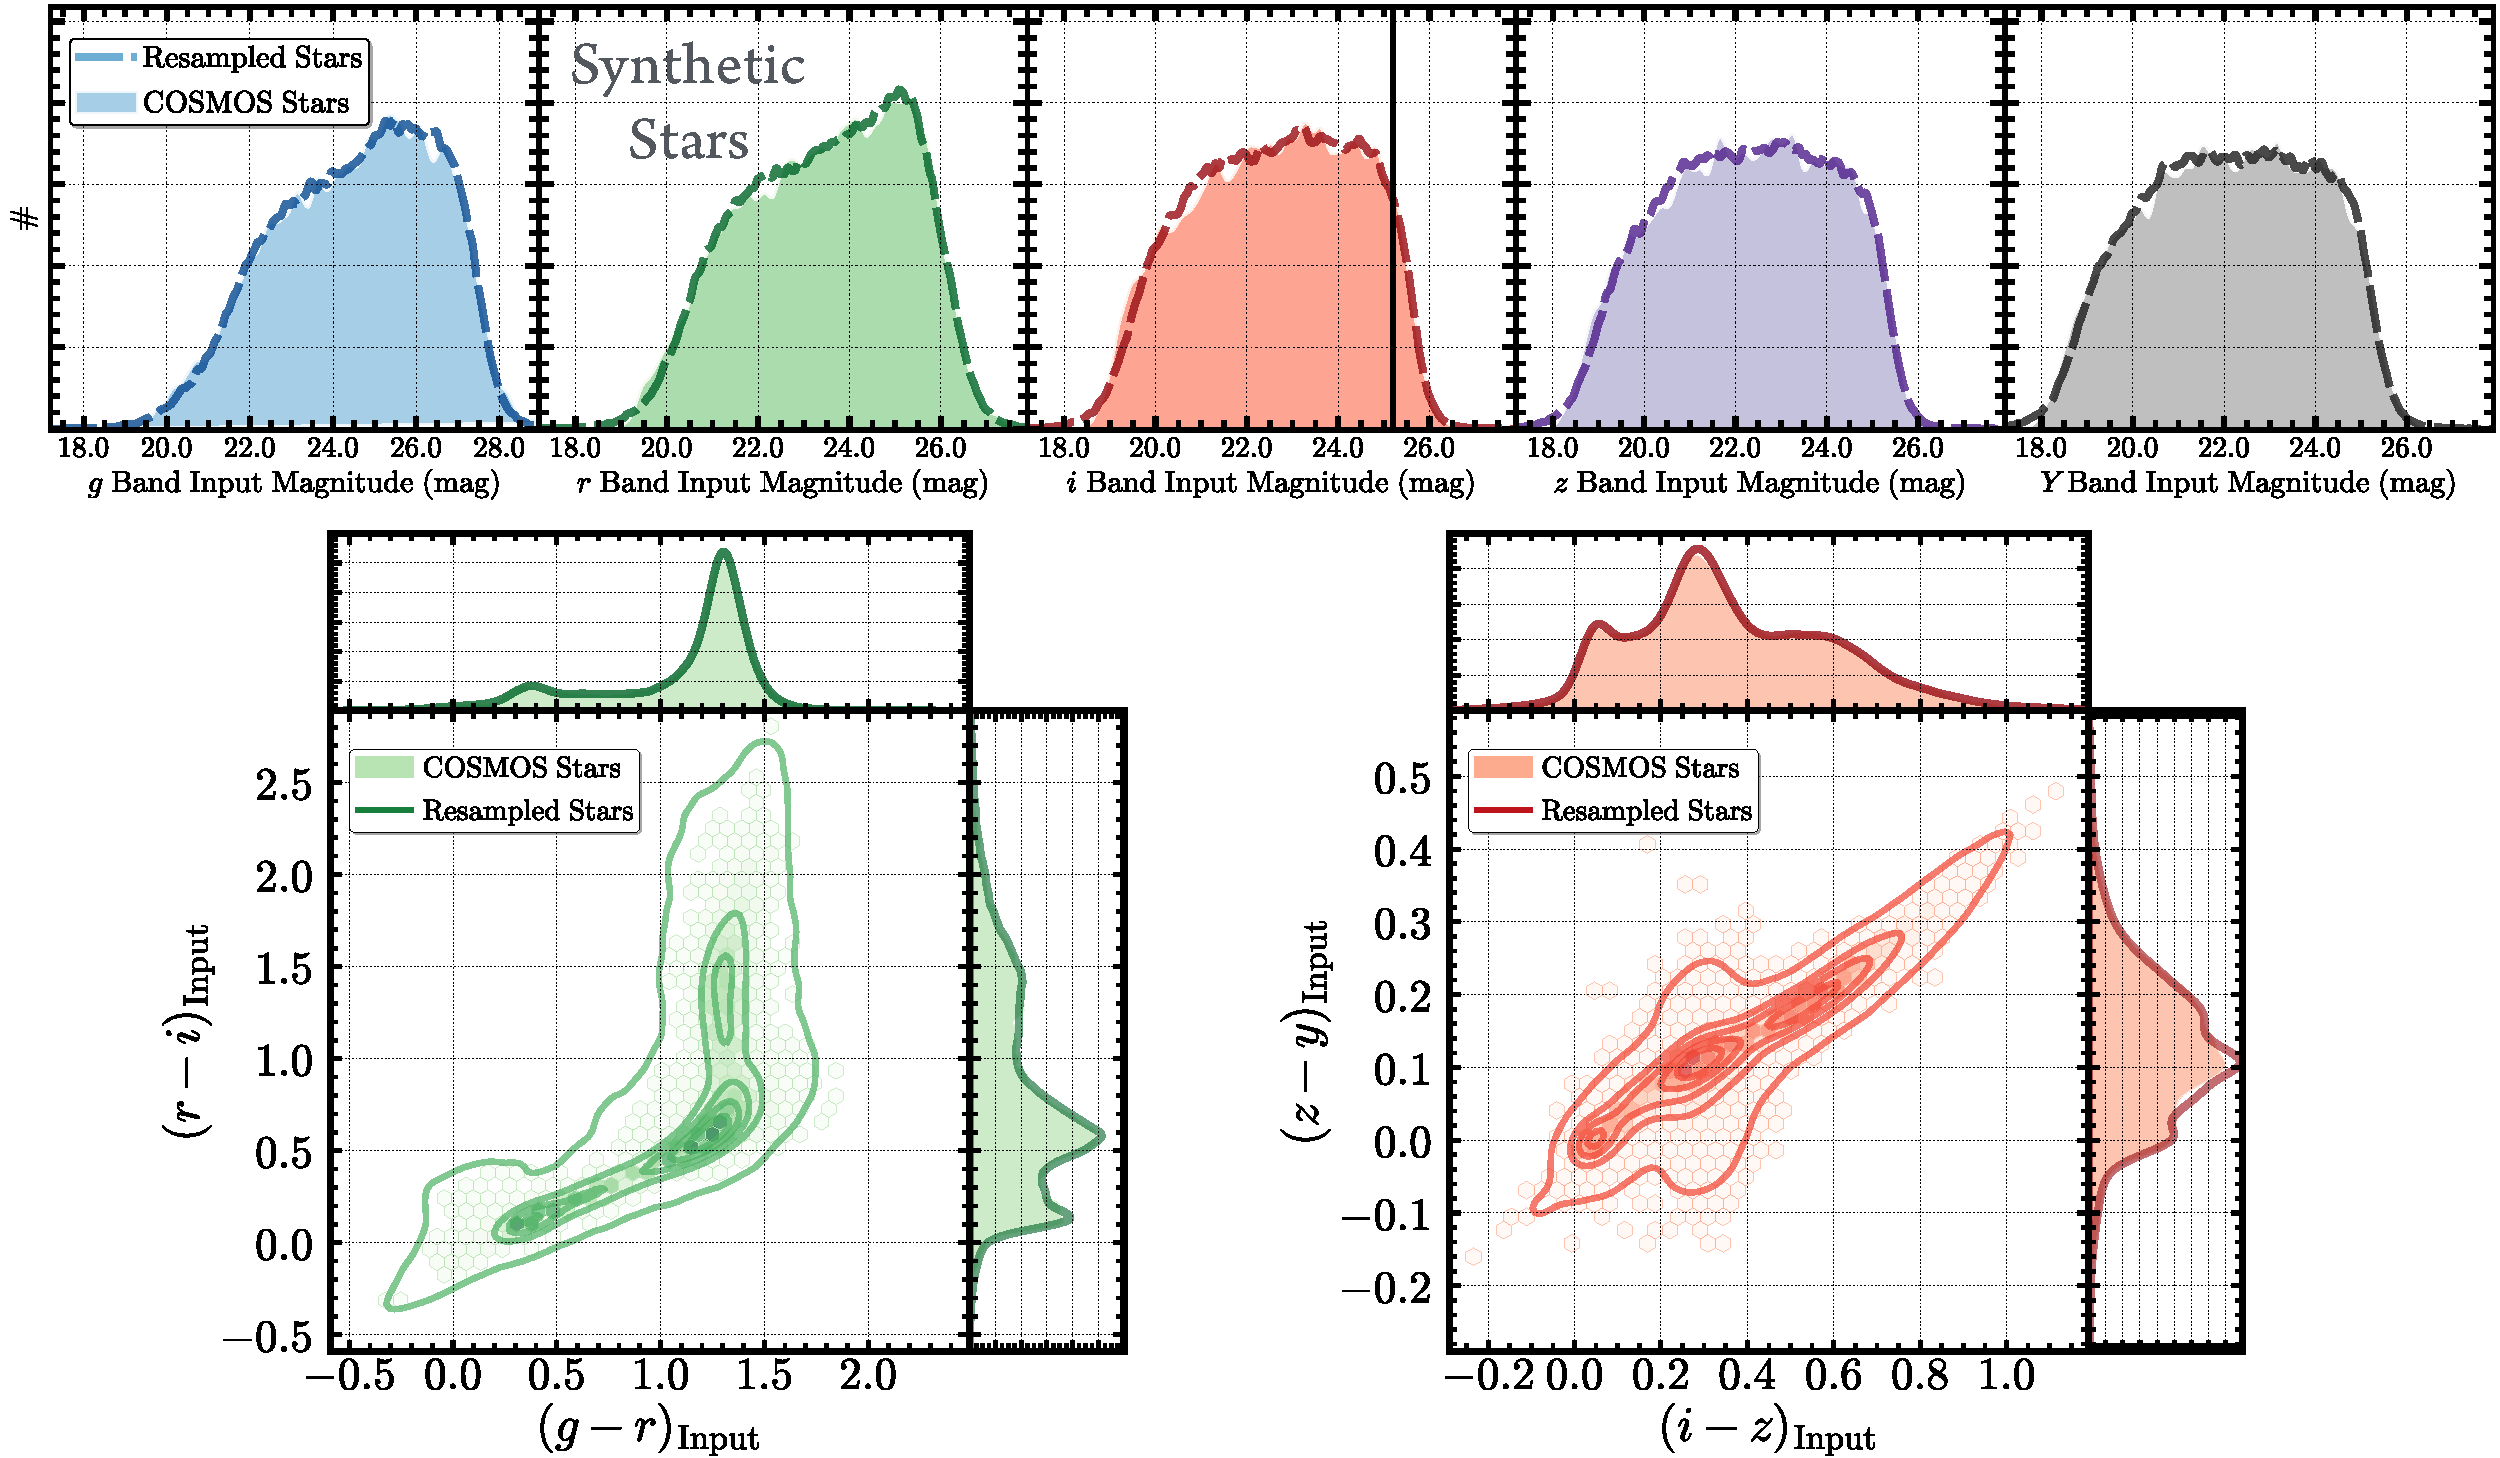
\includegraphics[width=\textwidth]{fig/synpipe_star_sample}
    \end{center}
    \caption{
        Magnitude and color distributions of synthetic stars.
        \textbf{Upper panel}: five-band magnitude distributions of the COSMOS
        stars (filled histograms) and  resampled stars (dashed lines).
        \textbf{Lower panel}: color-color distributions
        (left: $g-r$ v.s. $r-i$; right: $i-z$ v.s. $z-y$). Hexagonal bins indicate COSMOS stars and contours indicate resampled stars.}
    \label{fig:star_sample}
\end{figure*}
%% ------------------------------------------------------------------------------------ %%

%% ------------------------------------------------------------------------------------ %%
%% Fig: Galaxy Sample
\begin{figure*}
    \begin{center}
        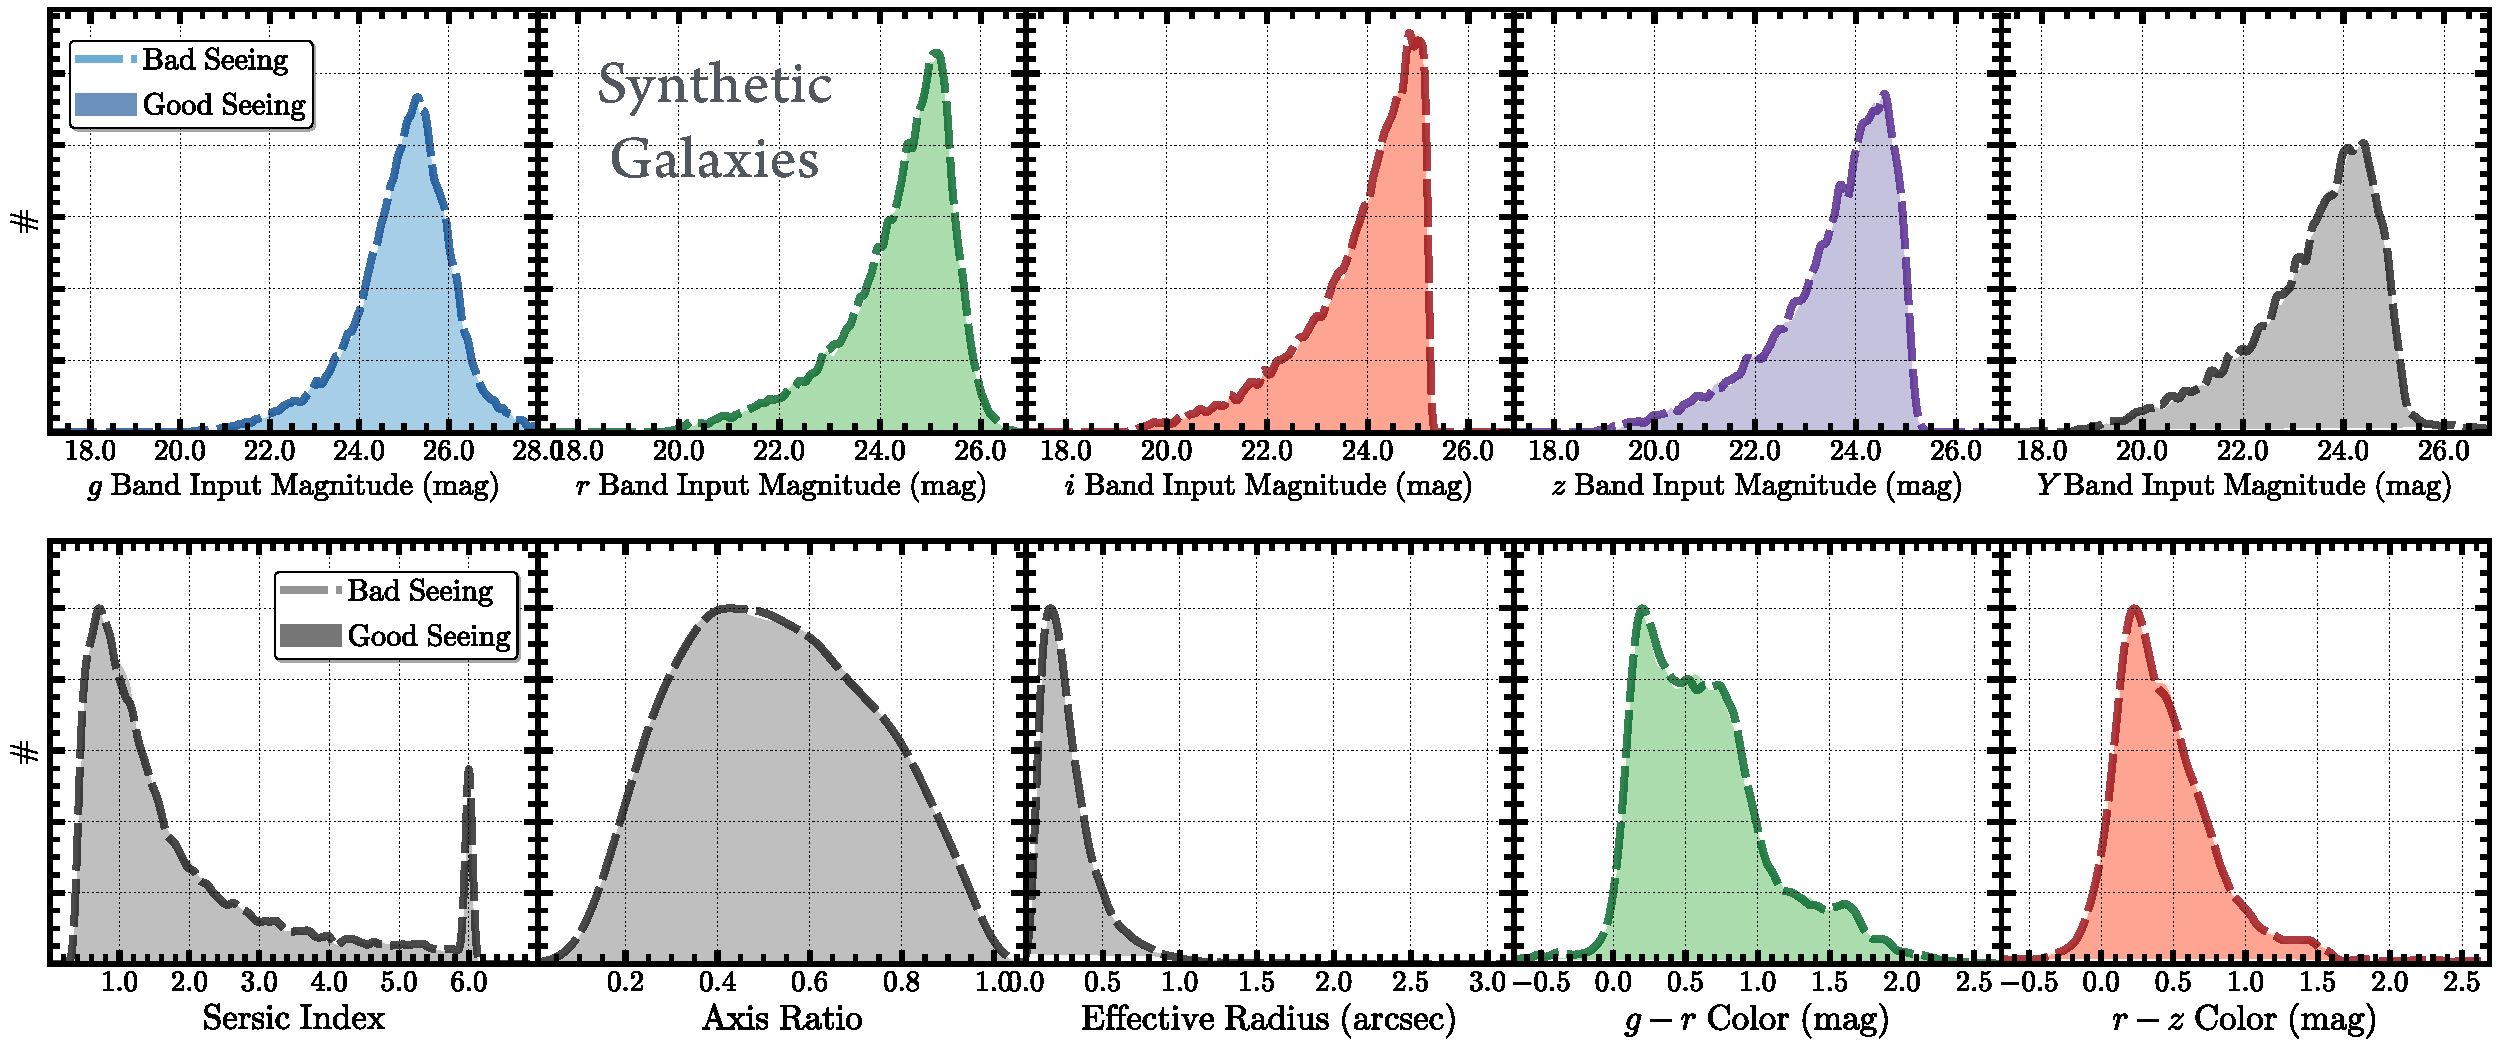
\includegraphics[width=\textwidth]{fig/synpipe_galaxy_sample}
    \end{center}
    \caption{ textbf{Upper panel}: five-band magnitude distributions of synthetic galaxies. (\texttt{lower panel}; from left to right are the \ser{} index, axis ratio,
        effective radius in arcsec, the $g-r$ and $r-z$ colors).}
    \label{fig:galaxy_sample}
\end{figure*}
%% ------------------------------------------------------------------------------------ %%

%% ------------------------------------------------------------------------------------ %%
\section{Generation of Synthetic Dataset}
    \label{sec:test}
    
    We now describe the  generation of the synthetic data set that we use to characterize the performance of \hscpipe{}.

%% ------------------------------------------------------------------------------------ %%
\subsection{Data}
    We use \tract{}$=9699$ in the VVDS field (median FWHM$=0.449$\asec{} in $i$-band;
    in this paper referred to as \texttt{goodSeeing}) and
    \tract{}$=8764$ in the XMM-LSS field (median FWHM$=0.700$\asec{};
    \texttt{badSeeing}).
    \tract{}$=9699$ also has better seeing in both $r$- and $z$-bands;
    the seeing conditions in $g$- and $y$-bands are very similar for both
    \tract{}$=9699$ and \tract{}$=8764$.
    For both \tracts{}, the \coadd{} image in each band includes data from
    20--40 \visits{}.  These  two \tract{} are selected  because they are not at the edge of a field, do not contain any  extremely bright ($i<12$ mag) saturated stars, and  are representative of both "good" and "bad" seeing conditions in the $i$-band.

%% ------------------------------------------------------------------------------------ %%

%% ------------------------------------------------------------------------------------ %%
\subsection{Input Models for Stars and Galaxies}
    \label{ssec:inputs}

We use a synthetic star sample built using data from  the HST/ACS catalog of \citet{Leauthaud2007}.  We first select stars from the  \citet{Leauthaud2007} catalog (this classification is reliable down to $I_{\mathrm{F814W}}{\sim}25.2$ mag). We then match this sample against our HSC UltraDeep--COSMOS data (which reaches ${\sim}27.2$ mag in $i$-band). After applying basic quality cuts (see \ref{app:qc}), this procedure  provides us with five-band HSC photometry for 14,472 stars. To increase the sample size, we re-sample the five-band magnitude distributions using the \texttt{astroML} (\citealt{astroml}) implementation of the \texttt{extreme-deconvolution} algorithm developed by
    \citet{Bovy2011}
    \footnote{\texttt{https://github.com/jobovy/extreme-deconvolution/}} to
    generate 100,000 synthetic stars. Fig \ref{fig:star_sample} shows the magnitude and color distributions of real COSMOS stars compared to the resampled distributions in all
    five-bands and in color-color space.

    For synthetic galaxies, we use single-\ser{} galaxy models of COSMOS galaxies with $I_{F814W} \leq 25.2$ mag. These are models from \citet{Lackner2012} applied to \textit{HST}/ACS images and are included in \galsim{}. Each model is described by a total of five parameters: magnitude, effective radius,
    \ser{} index, axis ratio, and position angle.
    Although the single-\ser{} model is not always the best choice for describing galaxies, its flexibility
    enables it to reasonably describe the flux distribution of most galaxies.
    Also, its simplicity makes it easy for us to diagnose potential problems with the \cmodel{} photometry.
    We exclude a tiny fraction of ill-behaved models that have a very high \ser{}
    index ($n_{\mathrm{Ser}} > 6.0$) or a very low central surface brightness
    ($\mu_{i} < 24.0$\sb).
    We further match this COSMOS sample with the HSC UltraDeep--COSMOS data.
    After removing objects with problematic photometry, we obtain a sample of
    58,210 synthetic galaxies with realistic five-band HSC photometry.
    As shown in Fig \ref{fig:galaxy_sample}, the majority of these galaxies are
    faint ($i<24.0$ mag) and barely resolved ($R_{\mathrm{e}}< 1.0$\asec).
    This sample is appropriate to test \hscpipe{}'s general photometric behaviors, but
    the sample lacks relatively bright galaxies ($i<20.5$ mag).

    We spatially distribute synthetic stars and galaxies randomly in our two selected \tracts{}. For stars, we use a number density of 1,000 per CCD. For galaxies, we use a number
    density of 500 per CCD.

%% ------------------------------------------------------------------------------------ %%

%% ------------------------------------------------------------------------------------ %%
\subsection{Generating \synpipe{} Data}
    \label{ssec:running}

    We use HSC DR1 data stored at Kavli Institute for the Physics and Mathematics of 
    the Universe (Kavli IPMU). For stars the \texttt{addFakes.py} step takes ${\sim}1.5$ hours per \tract{} in each
    band. The same process takes longer for galaxy tests (${\sim}3.0$ hours per
    \tract{} in each band) because the \galsim{} simulation is more time consuming.
    The \texttt{stack.py} step and \texttt{multiBand.py} step together take 
    ${\sim}3.5$ hours per \tract{}.

    We match the results with the input catalogs using a 2--pixel matching radius
    to generate output catalogs for \forced{} and \unforced{} photometry
    in each band. For our tests, we reject  synthetic objects  locate within 2 pixels of a real HSC object. 
    
    The detailed log of our runs can be found at \url{goo.gl/VINOVP}.
    The user should be able to reproduce the results presented in this work using 
    this information. It can also serve as a brief manual for generating \synpipe{} data.

%% ------------------------------------------------------------------------------------ %%

%% ------------------------------------------------------------------------------------ %%
\section{Photometric Performance Results}
    \label{sec:result}

    Here we discuss \hscpipe{}'s general performance, assessed mainly through \forced{} 
    PSF photometry (for stars) and (\cmodel{}) photometry (for galaxies).
    Although \hscpipe{} does provide other options (e.g., aperture and Kron photometry),
    these two are the only options that consider the effects of PSF in different bands 
    and are consistent across all bands in terms of position and shape. 
    
%% ------------------------------------------------------------------------------------ %%

%% ------------------------------------------------------------------------------------ %%
%% Fig: Magnitude v.s S/N for stars
\begin{figure*}
    \begin{center}
        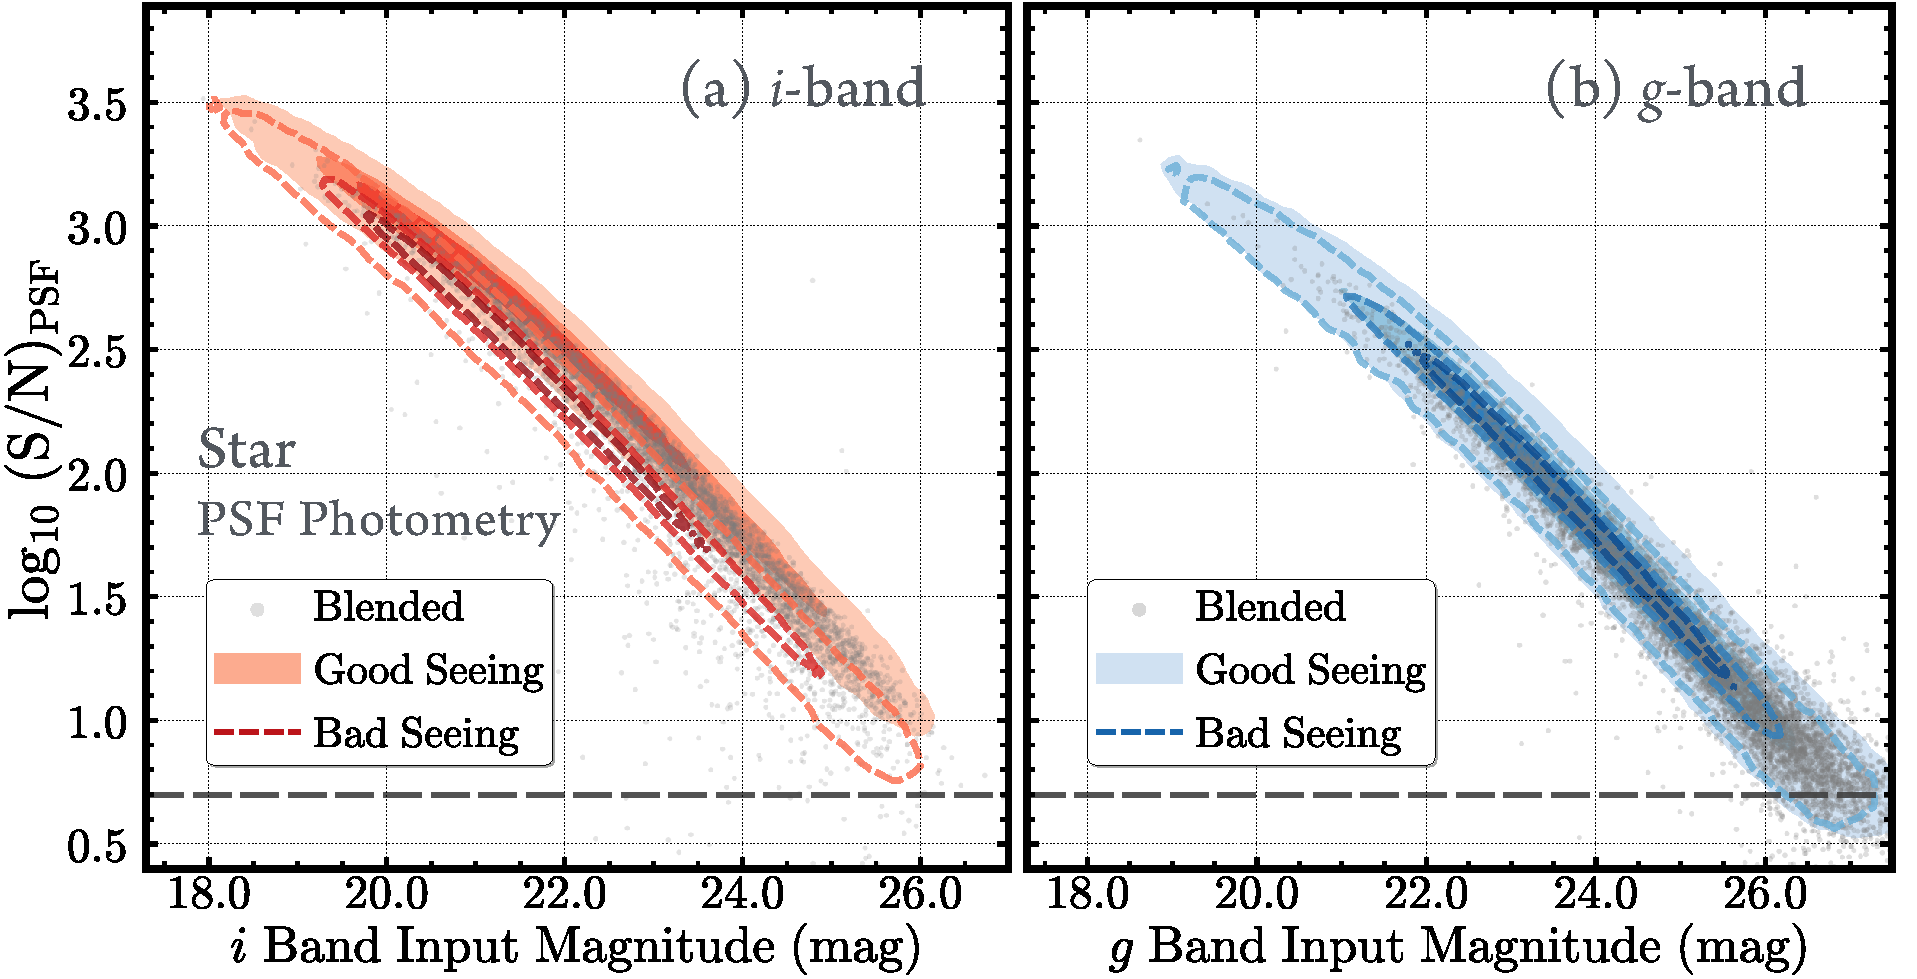
\includegraphics[width=\textwidth]{fig/synpipe_psf_sn}
    \end{center}
    \caption{
        Relation between input magnitudes (\textbf{left}: $i$-band; \textbf{right}:
        $g$-band) of synthetic stars and the $log(S/N)$ measured by \hscpipe{} PSF
        photometry.
        Hexagonal binned density plots and contours show the distributions for
        stars in both the good- and bad-seeing \tracts{}. Highly blended stars are highlighted using scatter plots.
        The gray dashed line marks $S/N = 5$ which is the detection threshold used by \hscpipe{}.  Our 5$\sigma$  point source detection limit  is \alexie{xxxx} however we do not reach these magnitudes with our current synthetic stellar input catalog.
        }
    \label{fig:star_sn}
\end{figure*}
%% ------------------------------------------------------------------------------------ %%

%% ------------------------------------------------------------------------------------ %%
%% Fig: Accuracy of Forced PSF Magnitudes
\begin{figure*}
    \begin{center}
        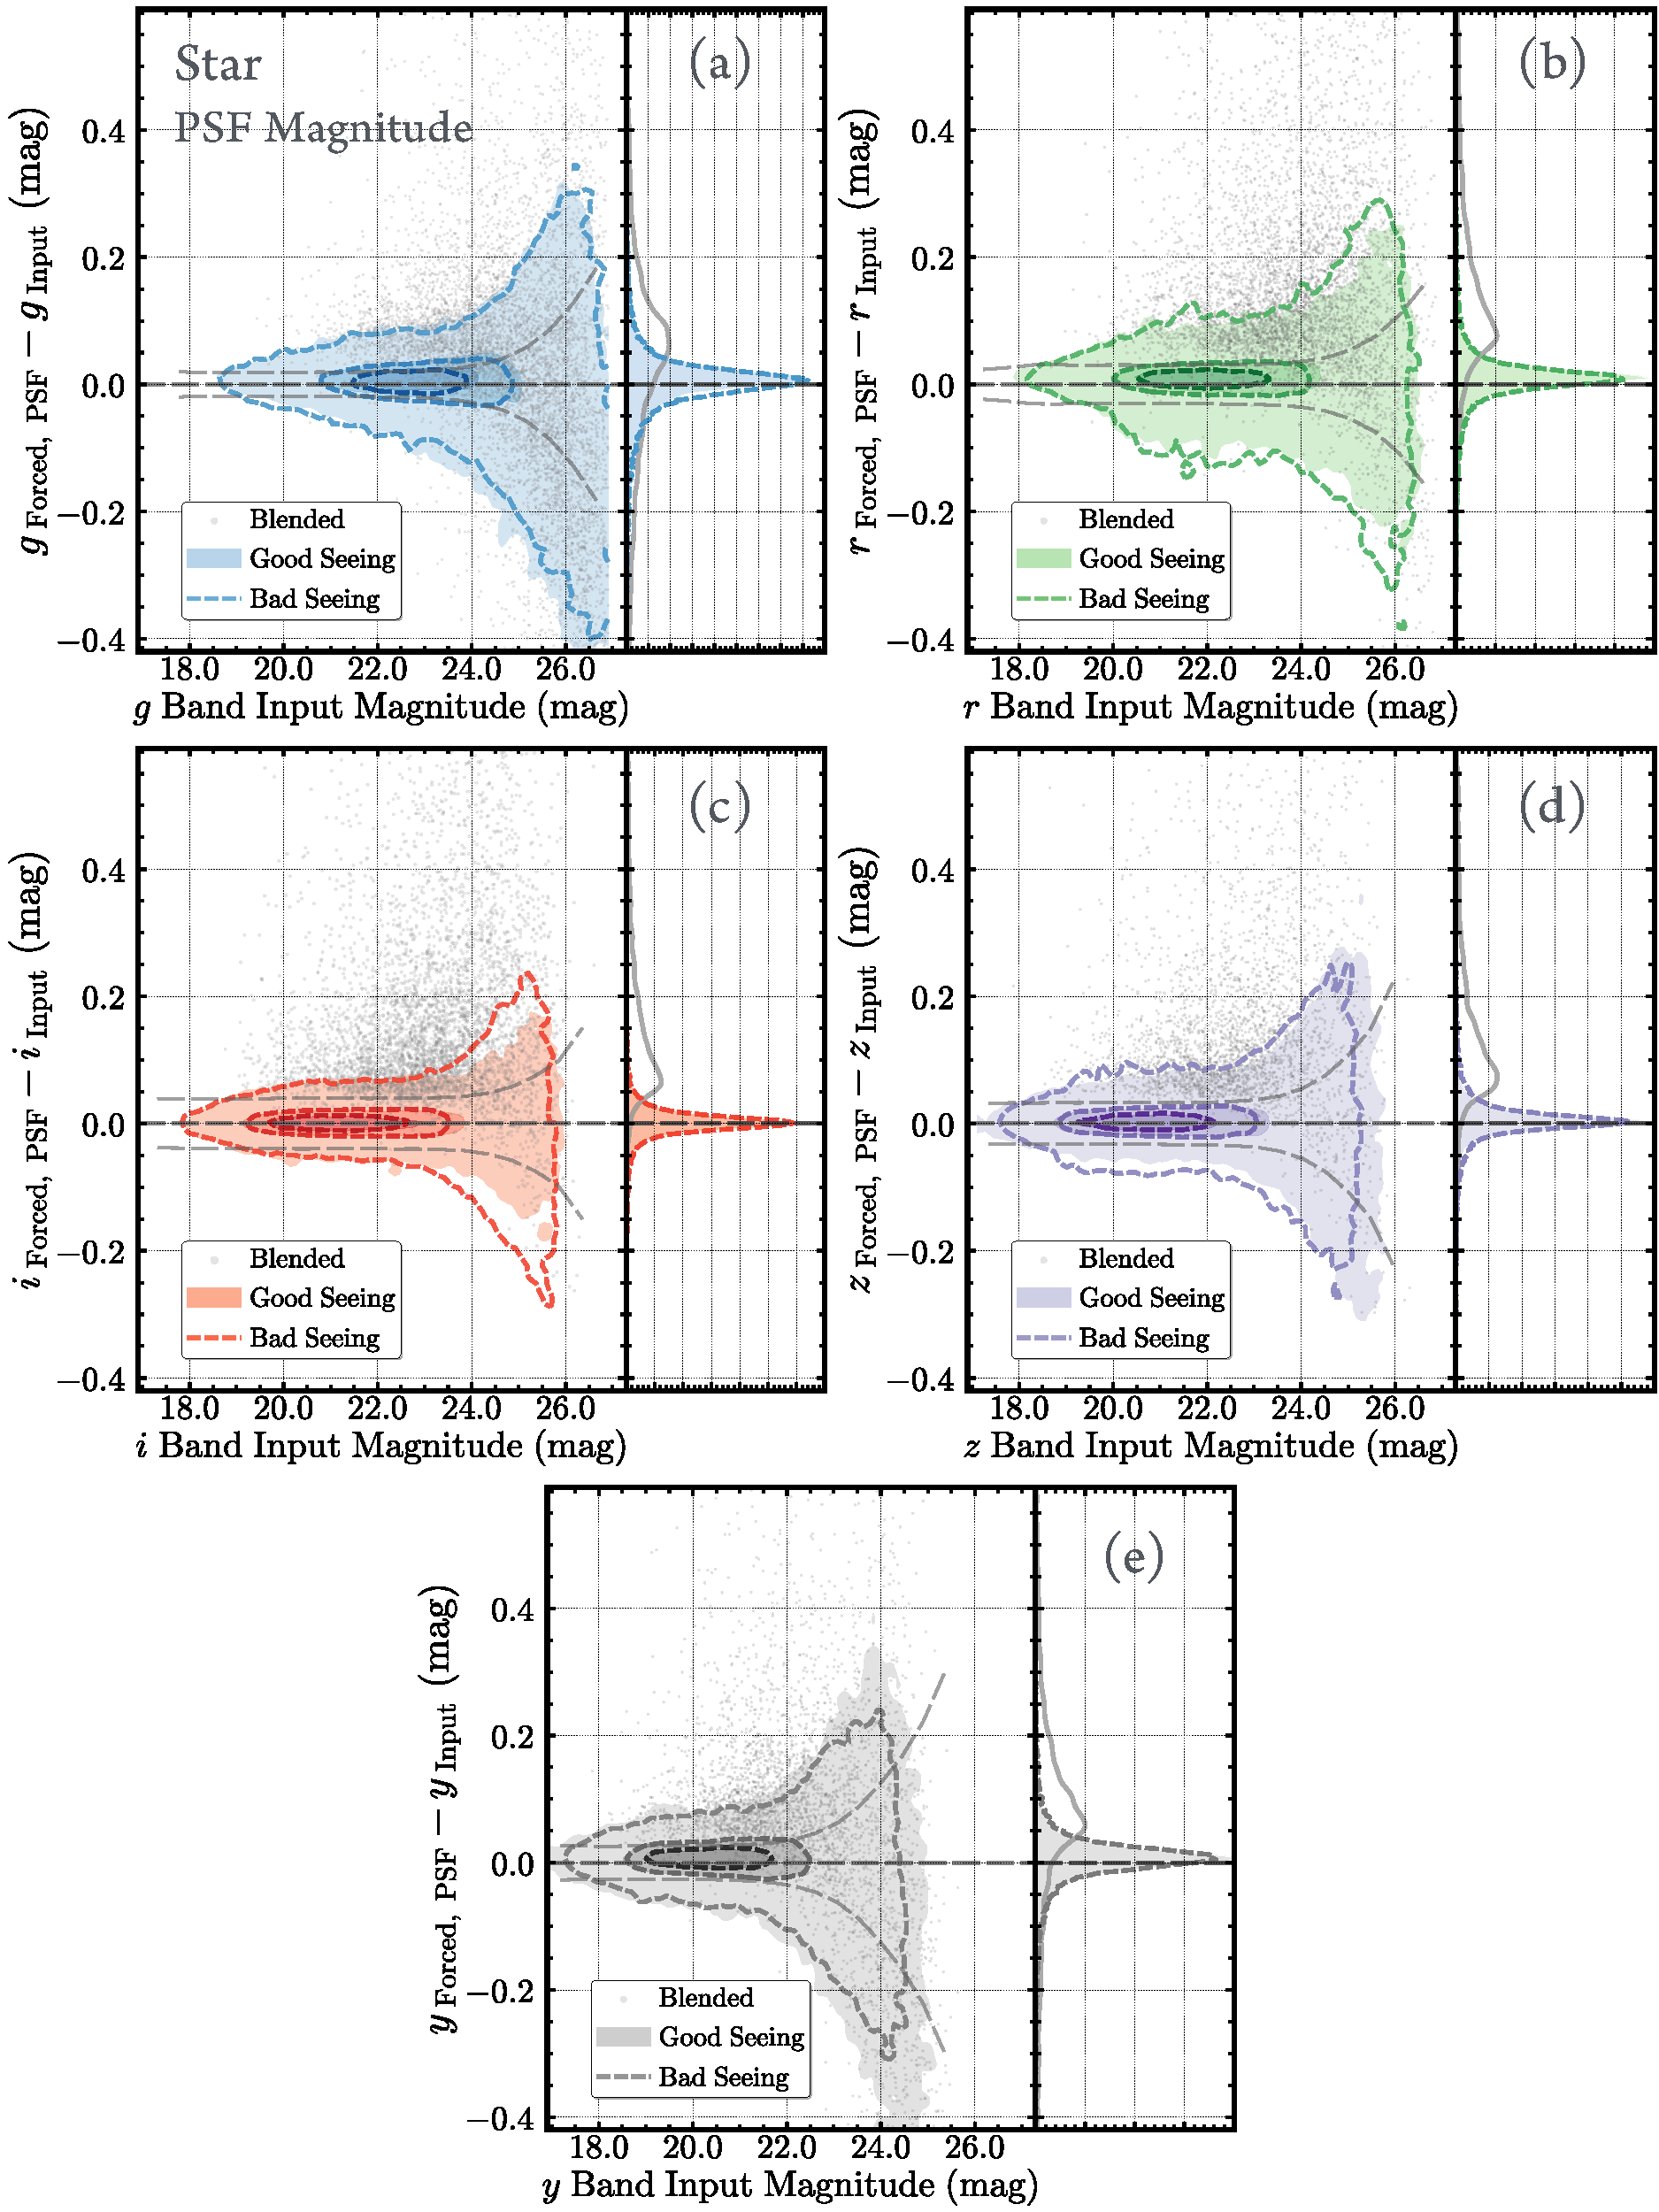
\includegraphics[width=16cm]{fig/synpipe_psf_mag}
    \end{center}
    \caption{
        Accuracy of the \texttt{hscpipe} PSF photometry for synthetic stars measured
        by the difference between input and output \forced{} PSF magnitudes.
        Plots [a, b, c, d, e] show the results for [$g$, $r$, $i$, $z$, $y$]-band, respectively.
        The left panel in each plot shows the relation between input magnitude and
        magnitude difference.
        Hexagonal binned density plots and contours are for the synthetic galaxies from
        good and bad seeing \tracts{}.
        Highly blended objects are highlighted using scattered plots.
        The long-dashed lines mark zero magnitude difference, while the pairs of
        dashed lines outline the running-median of PSF magnitude errors
        (including the uncertainties in aperture correction).
        The right panel in each plot shows the distributions of the magnitude differences for objects
        in good (filled) and bad (solid line) seeing \tracts{}.
        The dashed lines identify the distribution of highly blended objects.
        }
    \label{fig:psf_mag}
\end{figure*}
%% ------------------------------------------------------------------------------------ %%

%% ------------------------------------------------------------------------------------ %%
%% Fig: Difference between the Unforced and Forced Magnitudes
\begin{figure*}
    \begin{center}
        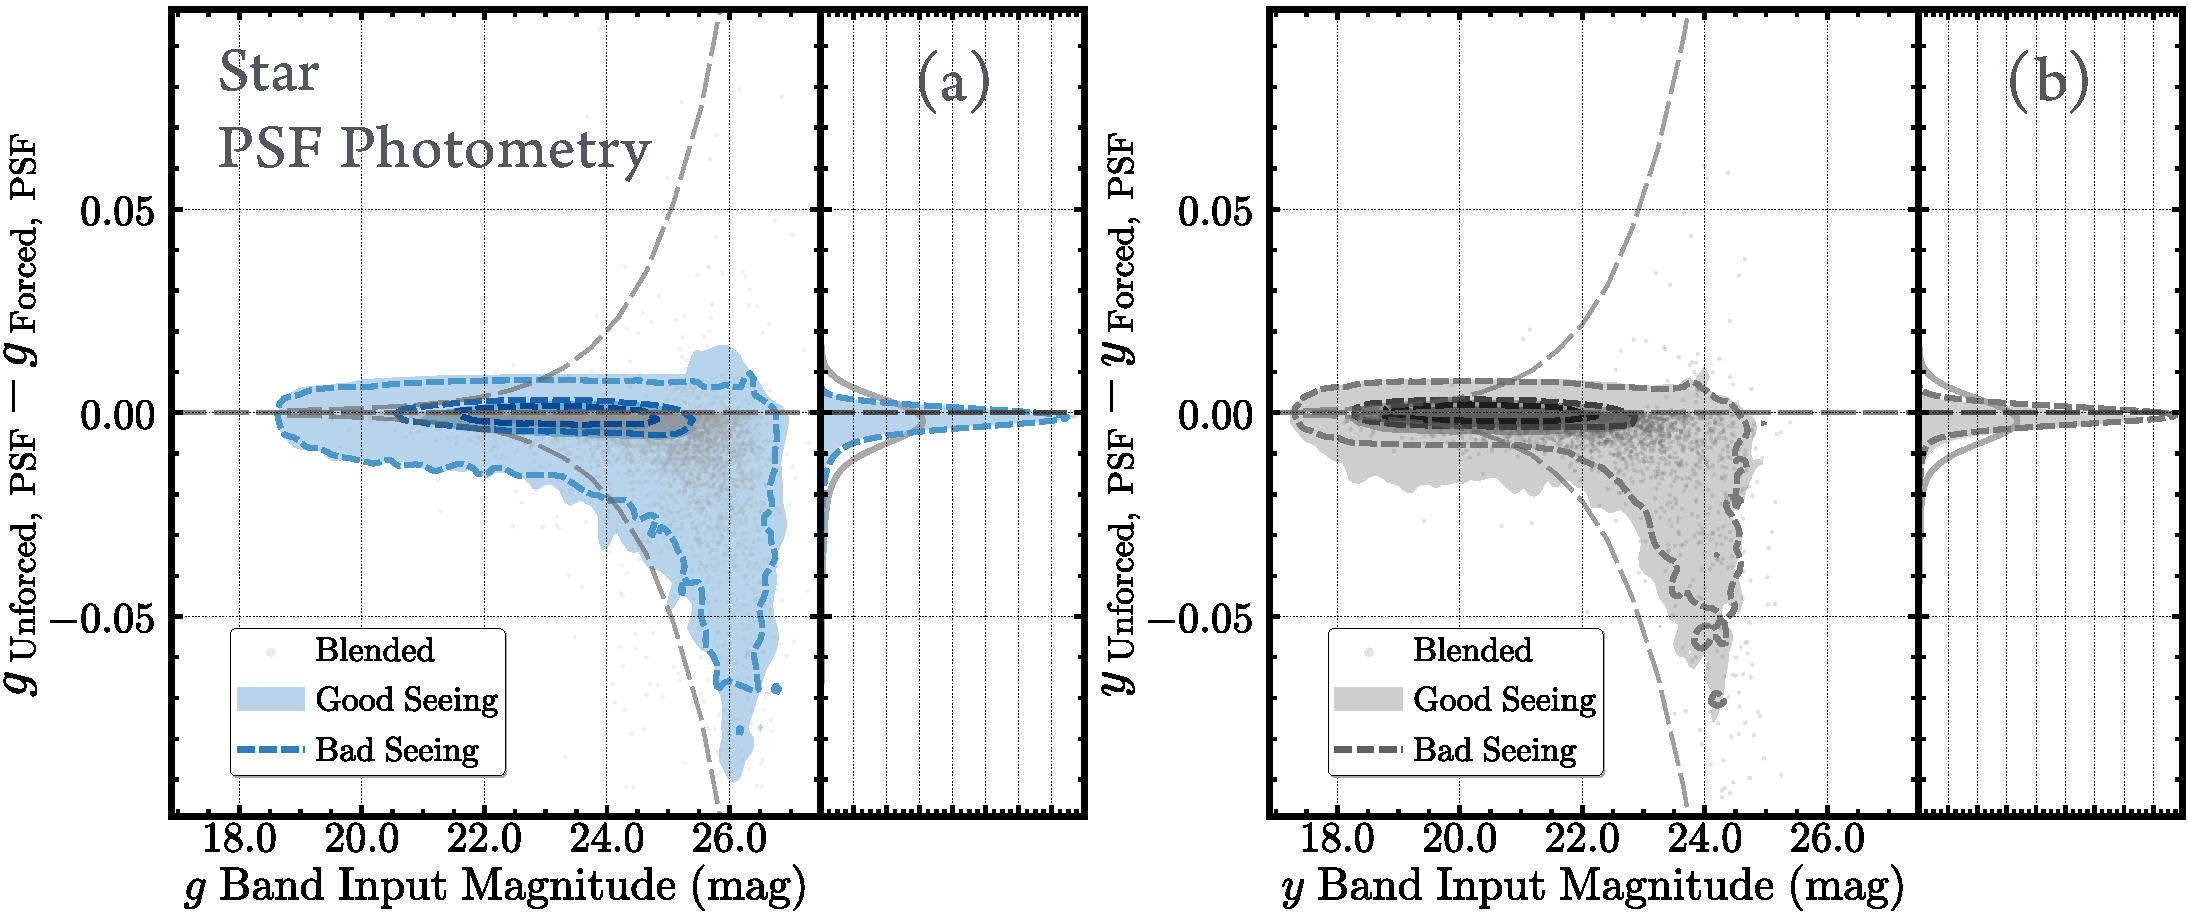
\includegraphics[width=\textwidth]{fig/synpipe_psf_diff}
    \end{center}
    \caption{
        The magnitude differences between the \unforced{} and \forced{}
        PSF photometry for synthetic stars in $g$- (\textbf{left} and $y$-band
        (\textbf{right}).
        The lines and contours legend is identical to the plots in Fig \ref{fig:psf_mag}.
        }
    \label{fig:psf_diff}
\end{figure*}
%% ------------------------------------------------------------------------------------ %%

%% ------------------------------------------------------------------------------------ %%
%% Fig: Accuracies of the PSF color
\begin{figure*}
    \begin{center}
        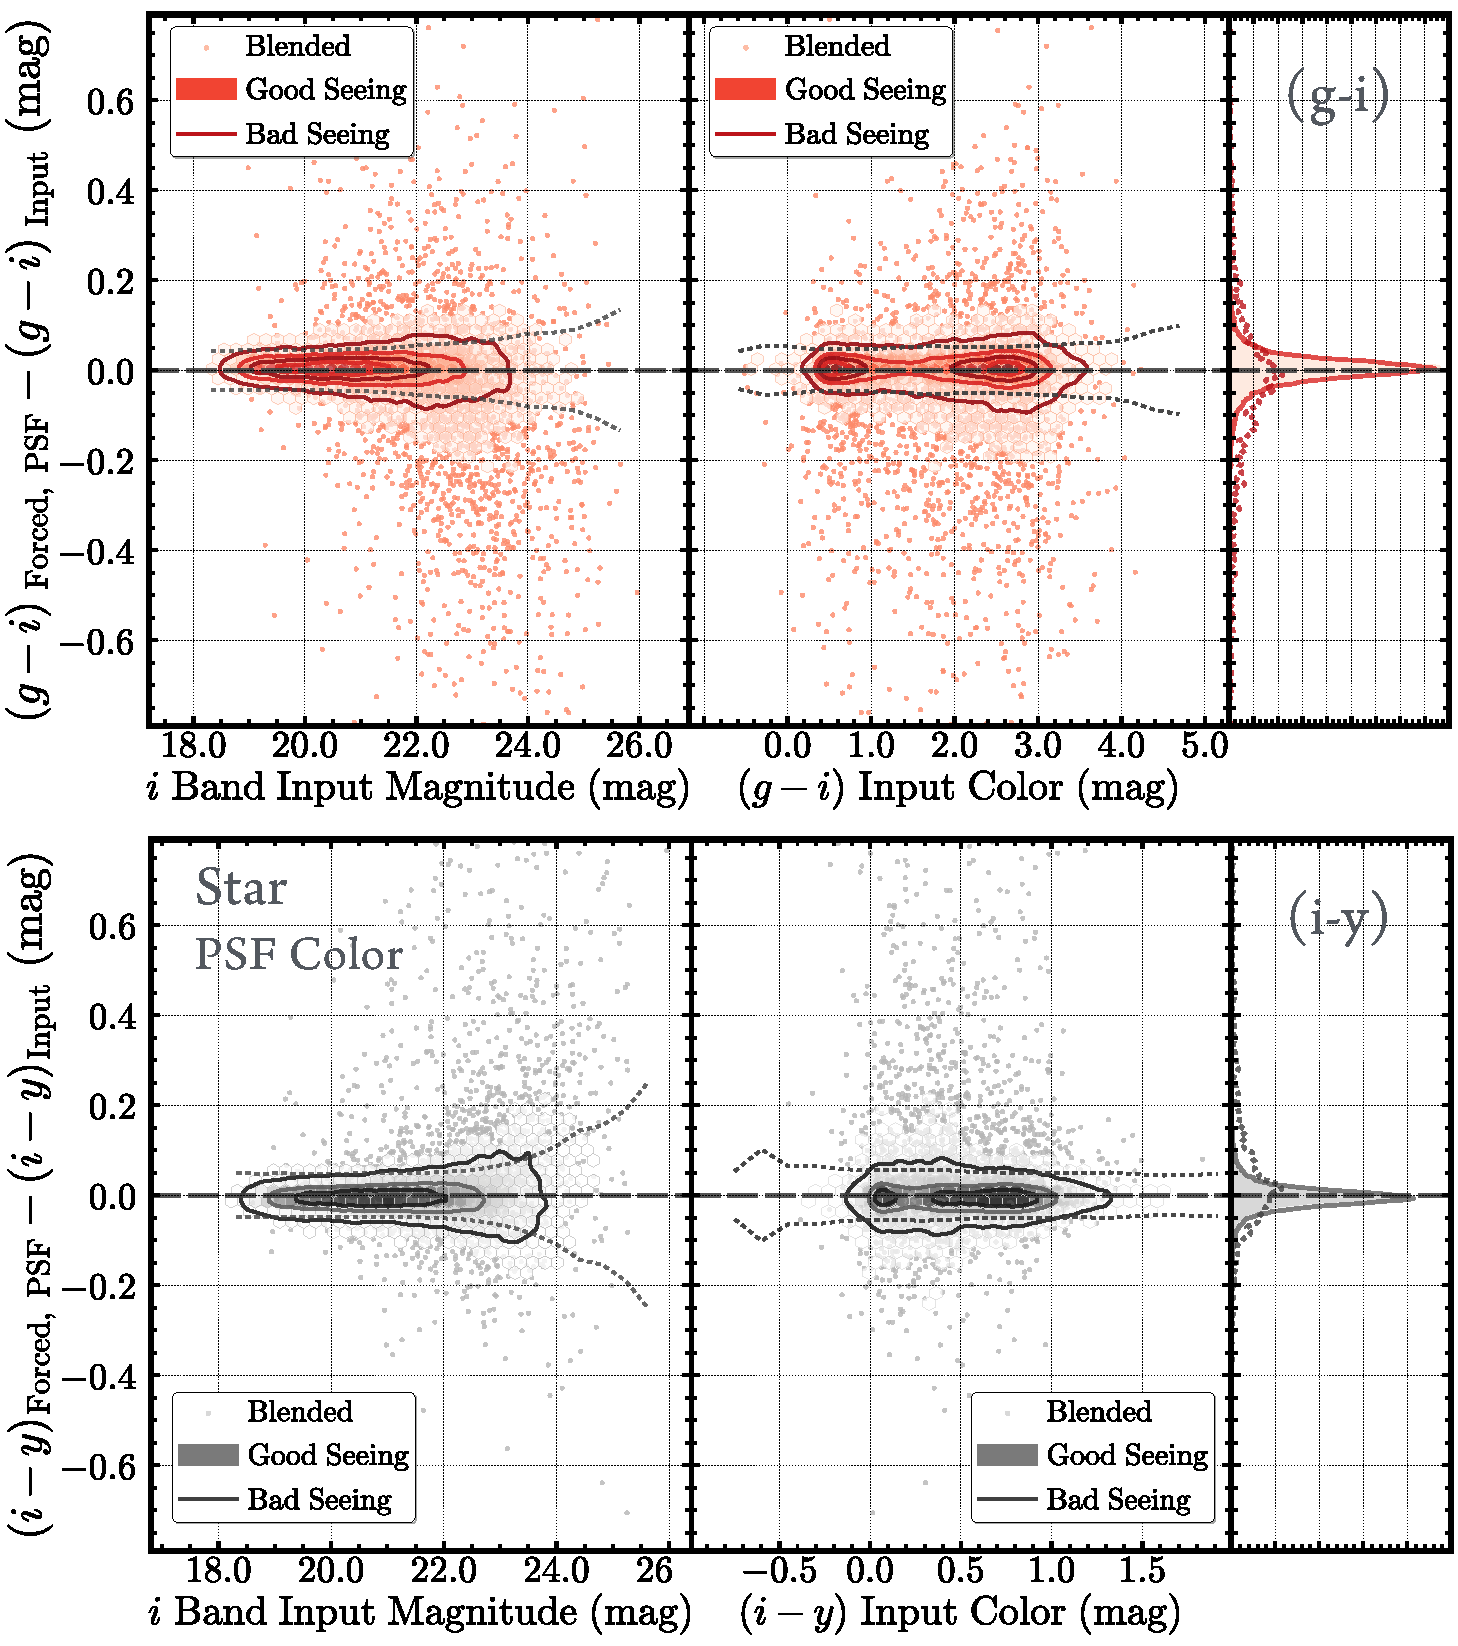
\includegraphics[width=\textwidth]{fig/synpipe_psf_color}
    \end{center}
    \caption{
        Accuracy of the color measurements for synthetic stars via the differences
        between input and \forced{} PSF colors.
        The \textbf{upper panels} and \textbf{lower panels} are for $g-i$ and $i-y$
        colors separately.
        The \textbf{left} column shows the relation between input magnitude and
        the color difference, and the \textbf{right} column uses the input colors as
        x--axis instead.
        The lines and contours legend is identical to the plot in Fig \ref{fig:psf_mag}.
        }
    \label{fig:psf_color}
\end{figure*}
%% ------------------------------------------------------------------------------------ %%

%% ------------------------------------------------------------------------------------ %%
%% Fig: Color-Color Distributions of the Input and Measurements for stars
\begin{figure*}
    \begin{center}
        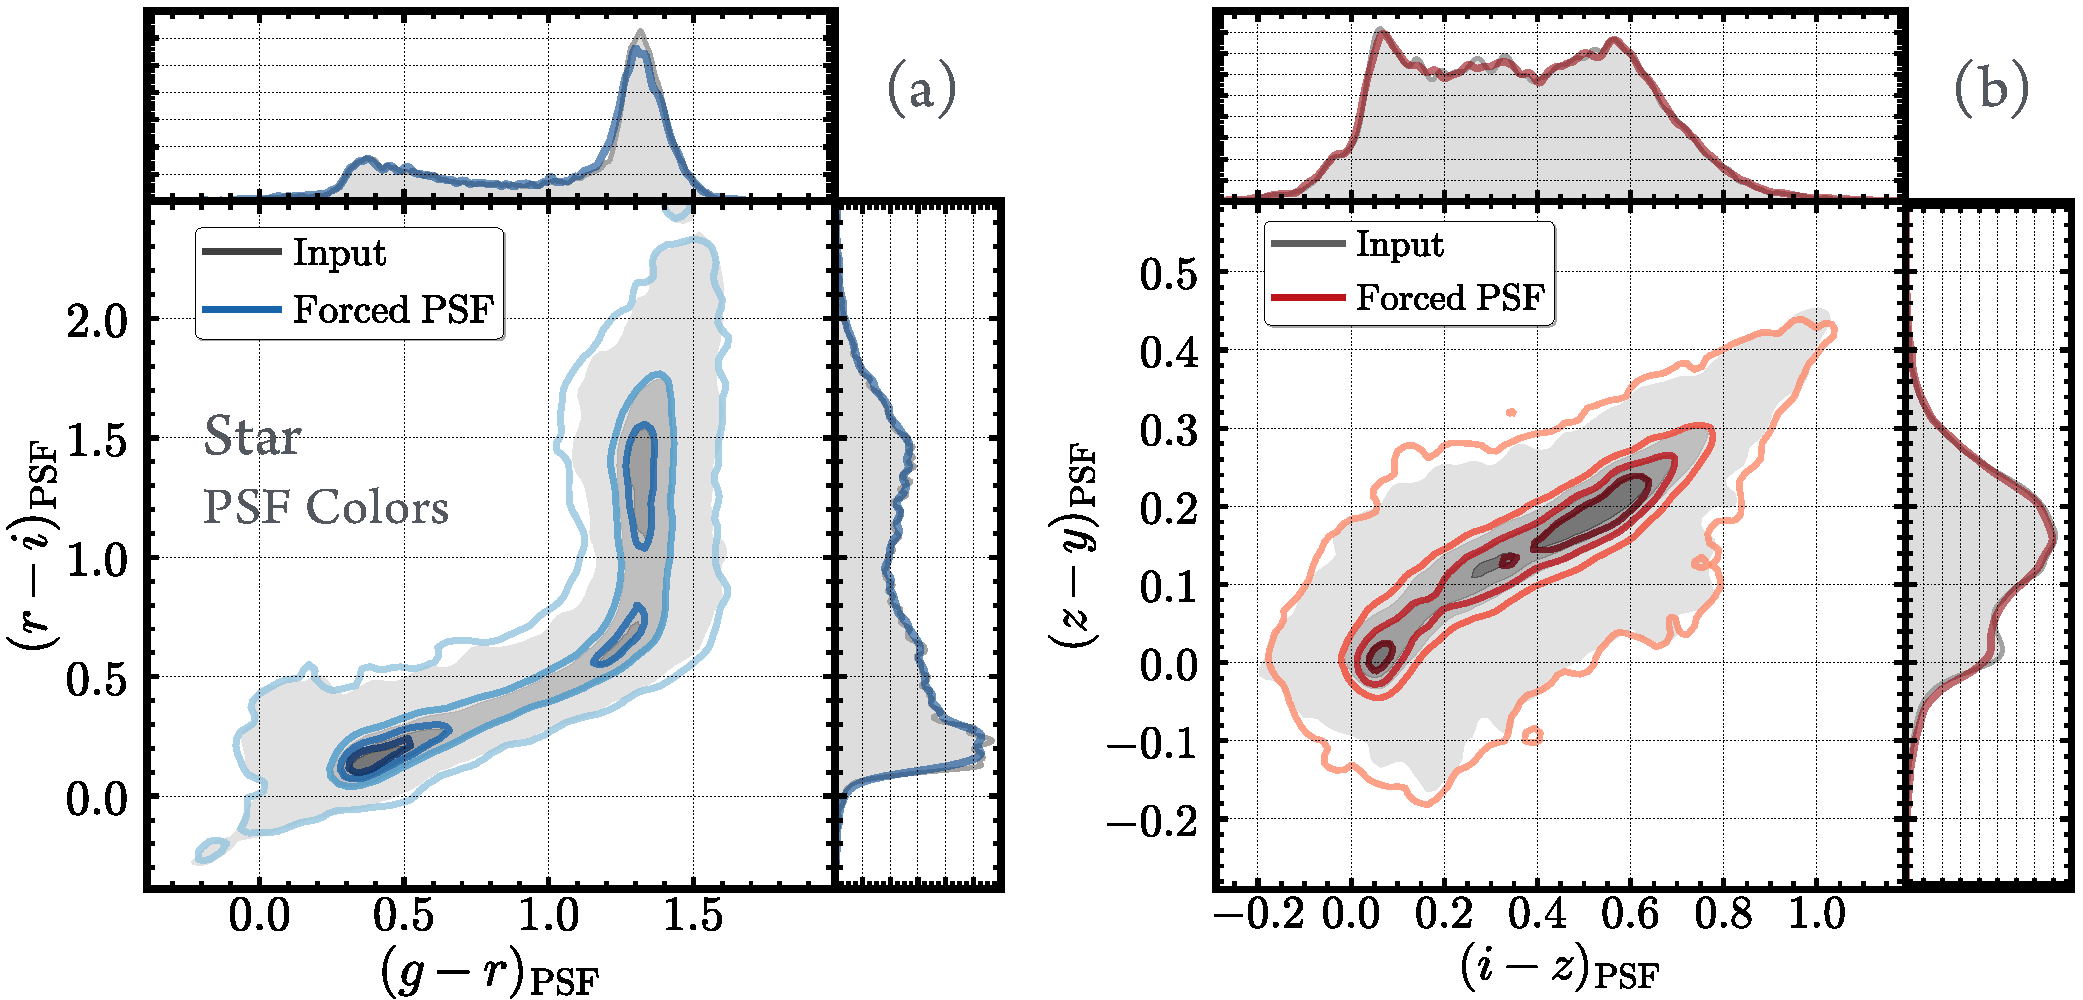
\includegraphics[width=\textwidth]{fig/synpipe_psf_cdist}
    \end{center}
    \caption{
        Evaluations of color measurement accuracy for synthetic stars using
        the color-color distributions.
       The plot on the \textbf{left} (a) uses $(g-r)$ v.s. $(r-i)$ colors, and the plot on the \textbf{right} (b)
        uses $(i-z)$ and $(z-y)$ colors.
        The filled contours and shaded histograms reflect the distributions for input
        colors.
        The empty contours and solid-line histograms show the distributions recovered
        by \hscpipe{}.
        }
    \label{fig:psf_cdist}
\end{figure*}
%% ------------------------------------------------------------------------------------ %%

%% ------------------------------------------------------------------------------------ %%
\subsection{PSF photometry of stars}
    \label{ssec:psf}

    In \hscpipe{}, the PSF magnitude is derived using a matched-filter method that
    depends on the best-fit PSF model and uses the Lanczos interpolation to shift
    the PSF model.
    The error of the PSF magnitude from \hscpipe{} only considers the per-pixel noise,
    and does not include centroid uncertainties.
    \hscpipe{} also estimates aperture correction for PSF photometry.
    For more details please see Bosch\etal (in prep.).

    We randomly inject ${\sim}100,000$ stars into each \tract{} in all
    five bands. Approximately ${\sim}3$--$4$\% of the stars are located within 2 pixels of the centroids
    of real objects; we remove those stars from the sample to avoid confusion in the comparisons. \alexie{xxxxxx}
 %   After this step, ${\sim}1$--$3$\% of the remaining synthetic stars still have no match in the \synpipe{} outputs.
 %   They could either be below the detection threshold or ambiguously blended with real objects \alexie{said you identified those}.
 %   The input $i$-band magnitudes of these unmatched stars are on average ${\sim}0.9$
 %   mag fainter than the matched ones.
 %   The fraction of unmatched stars is slightly higher in the bad seeing \tract{}; this result is consistent with our expectation that magnitude depends on seeing conditions,
 %   although the difference is not very significant \alexie{cut?}.
    For matched stars, we select the primary detections
    (\texttt{detect.is-primary=True}) that have good photometric quality
    (see Appendix \ref{app:qc} for details).
    This gives us ${\sim}83,000$ stars in each \tract{}.

    Next, we identify stars that are misidentified by \hscpipe{} as extended
    objects using the \texttt{classification.extendedness} parameter in each band.
    The fraction of misclassification is ${\sim}8$--$15$\%, and clearly depends on
    seeing conditions.
    For the same reason, $g$-band has the highest fraction of misclassification,
    while $i$-band is recommended for selecting point sources.
    The misclassified stars are on average ${\sim}1$ mag fainter than the others \alexie{xx}.
    We exclude them from the photometric comparison below, and further discuss
    the star--galaxy separation issue in Section \ref{ssec:sg}.

    In the following comparisons, we show the results from the
    \textbf{good-seeing} and \textbf{bad-seeing} \tracts{} separately because it
    is important to understand how the seeing condition affects photometric accuracy as well as to test whether \hscpipe{} can deliver unbiased photometry under different  seeing conditions.
    
    Besides seeing, the degree to which an object is blended with other objects  is another factor that influences photometric accuracy. To quantify the impact of blending effects, we use the ``blendedness'' parameter, $b$. This parameter describes how  much any given object overlaps with neighboring objects (see Appendix \ref{app:defineb} and Murata\etal in prep.). We divide our sample  according to the  blendedness parameter. A value of $b=0$ corresponds to isolated objects whereas  objects with $b=1$ complete overlap with other objects. Here we use $b>0.05$ to define highly blended stars (${\sim}4$--$9$\% are blended).
    The fraction of highly blended stars slightly increases in the bad seeing \tract{}. The
    impact of blendedness will be discussed more in Section \ref{ssec:blendedness}.

\subsubsection{Relationship between stellar magnitude and \s2n{}}

\alexie{TO HERE}

We define the  \s2n{} for PSF photometry as
    $\mathrm{Flux}_{\mathrm{PSF}}/\mathrm{Flux\_Err}_{\mathrm{PSF}}$ in each band
    without considering aperture corrections.
    This helps us visualize
    1) the detection limit for point sources,
    2) the impact of seeing condition on PSF photometric,
    3) and the scatter of photometric accuracies at a fixed input magnitude given all
       the realistic features of HSC images (e.g., background subtraction, nearby
       objects, optical artifacts).
    We show the results for $g$- and $i$-bands in Fig \ref{fig:star_sn}, and find close
    relations in both bands.

    As expected, we clearly see that the seeing condition impacts the \s2n{} of point
    sources at fixed input magnitude.
    In  $i$-band, the bad-seeing (0.7\asec{}) \tract{}  shows systematically
    lower \s2n{} than the good-seeing (0.5\asec{}) \tract{}.
     \s2n{} is similar for the two $g$-band \tracts{} because they share similar seeing conditions.
    Our results show that blendedness can also affect the accuracy of PSF photometry.
    In $i$-band, the highly blended synthetic stars scatter toward lower \s2n{} at
    fixed magnitude.
    Interestingly, the effect is not obvious in $g$-band, suggesting the deblending
    process and photometric quality of blended objects also depend on seeing condition.

    At \s2n{}$=5$, HSC Wide can detect stars as faint as ${\sim}26.5$ mag in both $g$- and
    $i$-bands, which is consistent with the values found
    in \citet{HSCDR1} for average seeing conditions.
    At the same time, it is worth reminding HSC data users that the detection
    limit will show spatial variations due to the seeing conditions.

\subsubsection{Accuracy of PSF magnitude}

    Now, we look into PSF magnitude accuracy in each of the five bands
    independently.
    Fig \ref{fig:psf_mag} shows the relation between the input magnitude and the
    magnitude difference from the \hscpipe{} \forced{} PSF photometry.

    The overall performance of PSF photometry is excellent.
    In $i$-band, the median magnitude difference for \tract{} with 0.45\asec{} seeing is
     ${\sim}0.015$ mag (${\sim}1.5$\% accuracy) at
    $i_{\mathrm{Input}}{\sim}19.0$ mag.
    At $i_{\mathrm{Input}}{\sim}24.0$ mag, the average accuracy of PSF
    magnitude holds at ${\sim}3$\% level (${\sim}0.036$ mag average difference).
    At $i_{\mathrm{Input}}{\sim}25.2$ mag, the average accuracy decreases to
    ${\sim}7$\% level with an average ${\sim}0.072$ mag difference.
    The bad-seeing \tract{} shows similar accuracy of PSF photometry at
    $i_{\mathrm{Input}}<23.5$ mag.
    At the faint end, the accuracy becomes slightly worse: ${\sim}5$\% accuracy around
    $i_{\mathrm{Input}}{\sim}24.0$ mag and ${\sim}11$\% accuracy around
    $i_{\mathrm{Input}}{\sim}25.2$ mag.
    \citet{HSCDR1} evaluates the accuracy of PSF photometry via external comparisons
    with the PS1, PV2, and SDSS data at $i<21$ mag, and finds a 1-2\% level accuracy,
    which is consistent with our results.
    At fainter magnitude, external comparisons become difficult due to the lack of deep
    imaging data at HSC level and also due to the impact of the color-term when comparing photometry
    using different filters.
    The results from \synpipe{} hence provide more useful evaluations down to the
    detection limit\footnote{Strictly speaking, the uncertainties here should be
    considered as the lower limit because \synpipe{} currently does not consider the uncertainties
    in PSF modeling.}.

    We also see that the accuracy of PSF photometry does not strongly depend on filters.
    The accuracy of the forced PSF magnitude in $r$- and $z$-bands is similar to
    $i$-band observations (1.5-4.0\% at $19.0 < r_{\mathrm{Input}} < 24.0$ mag, ${\sim}8$\% down to
    $r_{\mathrm{Input}}{\sim}25.2$ mag;
    1.0-5.0\% at $19.0 < z_{\mathrm{Input}} < 24.0$ mag, ${\sim}10$\% down to
    $z_{\mathrm{Input}}{\sim}25.2$ mag).
    The accuracies in $g$- and $y$-bands become slightly worse (1.5-7.0\% at $19.0 < g_{\mathrm{Input}} < 24.0$ mag, ${\sim}13$\% down to
    $g_{\mathrm{Input}}{\sim}25.2$ mag;
    1.5-5.0\% at $19.0 < y_{\mathrm{Input}} < 23.0$ mag, ${\sim}12$\% down to
    $y_{\mathrm{Input}}{\sim}24.0$ mag;); however, the differences can be attributed to the
    differences in seeing conditions.

    For relatively isolated stars, \hscpipe{} provides unbiased PSF photometry down to a
    very faint magnitude in $i$- and $z$-bands.
    For $g$-, $r$-, and $y$-bands, we find small offsets in the distributions of magnitude
    differences, which indicates \hscpipe{} tends to underestimate the fluxes of stars
    in these bands by ${\sim}0.01-0.02$ mag.
    Although the exact cause of this offset is unclear (it could be related to
    differences in seeing), it will not affect the accuracies of magnitudes or colors.

    At the same time, the story for highly blended stars is very different.
    \hscpipe{} on average systematically underestimates their total fluxes by
    $0.05$--$0.10$ mag at a fixed input magnitude.
    We see the same effect in all bands, and the impact of blendedness becomes
    increasingly significant at fainter magnitude.
    It is important to keep this in mind when using PSF photometry for point
    sources in HSC data.

    We also test the \unforced{} PSF photometry in all five bands, and find very similar
    accuracies.
    While measuring \forced{} PSF photometry, \hscpipe{} fixes the centroid
    of the PSF model across all five bands.
    Therefore, the  difference between \forced{} and \unforced{} PSF magnitudes
    indicates the photometric uncertainties induced by the differences in the accuracies of
    astrometric calibrations and PSF modeling among different bands.
    We highlight the differences between \forced{} and \unforced{} PSF photometry of
    $g$- and $y$-bands in Fig \ref{fig:psf_diff}.
    The overall difference is very small ($<0.01$ mag), but it also suggests that
    \hscpipe{} \unforced{} PSF photometry systematically recovers slightly more fluxes
    at the very faint end.

\subsubsection{Accuracy of the PSF colors}

    PSF photometry is the most appropriate way to measure colors for point
    sources; therefore, the accuracy of the PSF color estimates is important to many scientific goals of the HSC survey
    (e.g., study of the Milky Way structure, selection of unique stellar objects or
    high-redshift quasars, and accurate star--galaxy separation).

    In Fig \ref{fig:psf_color}, we evaluate the accuracies of the \forced{} $(g-i)$
    and $(i-y)$ PSF colors via comparing the error in color measurements with both
    input magnitudes and input colors.
    These results suggest that \hscpipe{} provides accurate and unbiased PSF color
    estimates for synthetic stars with realistic color distributions down to a very faint
    magnitude.
    For $(g-i)$ color, the average uncertainty around $i_{\mathrm{Input}}{\sim}19.0$ mag
    is ${\sim}0.025$ mag, and increases to ${\sim}0.11$ mag at
    $i_{\mathrm{Input}}{\sim}24.0$ mag.
    The results are very similar for the $(i-y)$ color.
    We also find that the accuracies of PSF colors do not depend on the input colors of
    the synthetic stars or the seeing conditions.
    For instance, the accuracy of $(g-i)$ color for a bad-seeing \tract{} is only
    slightly worse in the very faint end (${\sim}0.14$ mag at
    $i_{\mathrm{Input}}{\sim}24.0$ mag) compared to the results for a good-seeing \tract{}.

    We further illustrate the accuracies of PSF colors via comparing the distributions
    of colors for the input synthetic stars and the stars recovered by \hscpipe{}
    (see Fig \ref{fig:psf_cdist}).
    Using four different colors and two 2--D color--color planes, we show that the \forced{}
    PSF colors can accurately reproduce the distributions of all four colors and the
    2-D color-color distributions.

    As for the highly blended stars, on Fig \ref{fig:psf_color}, we see that on average
    they still have larger uncertainties in colors compared to the relatively isolated
    ones.
    For $(g-i)$ color, the average color uncertainty is ${\sim}0.1$ mag larger for the
    highly blended stars at a fixed input magnitude.
    However, the biases in color measurements for these stars are less severe than
    the magnitude measurements.
    Although the blended stars still show slightly bluer color for $(g-i)$ and slightly redder color for $(i-y)$
    compared to the isolated stars and the input values, the differences in the
    distributions of color uncertainties of blended and isolated stars are less striking
    than the distribution differences for magnitude.

%% ------------------------------------------------------------------------------------ %%

%% ------------------------------------------------------------------------------------ %%
%% Fig: Magnitude v.s S/N for galaxies
\begin{figure*}
    \begin{center}
        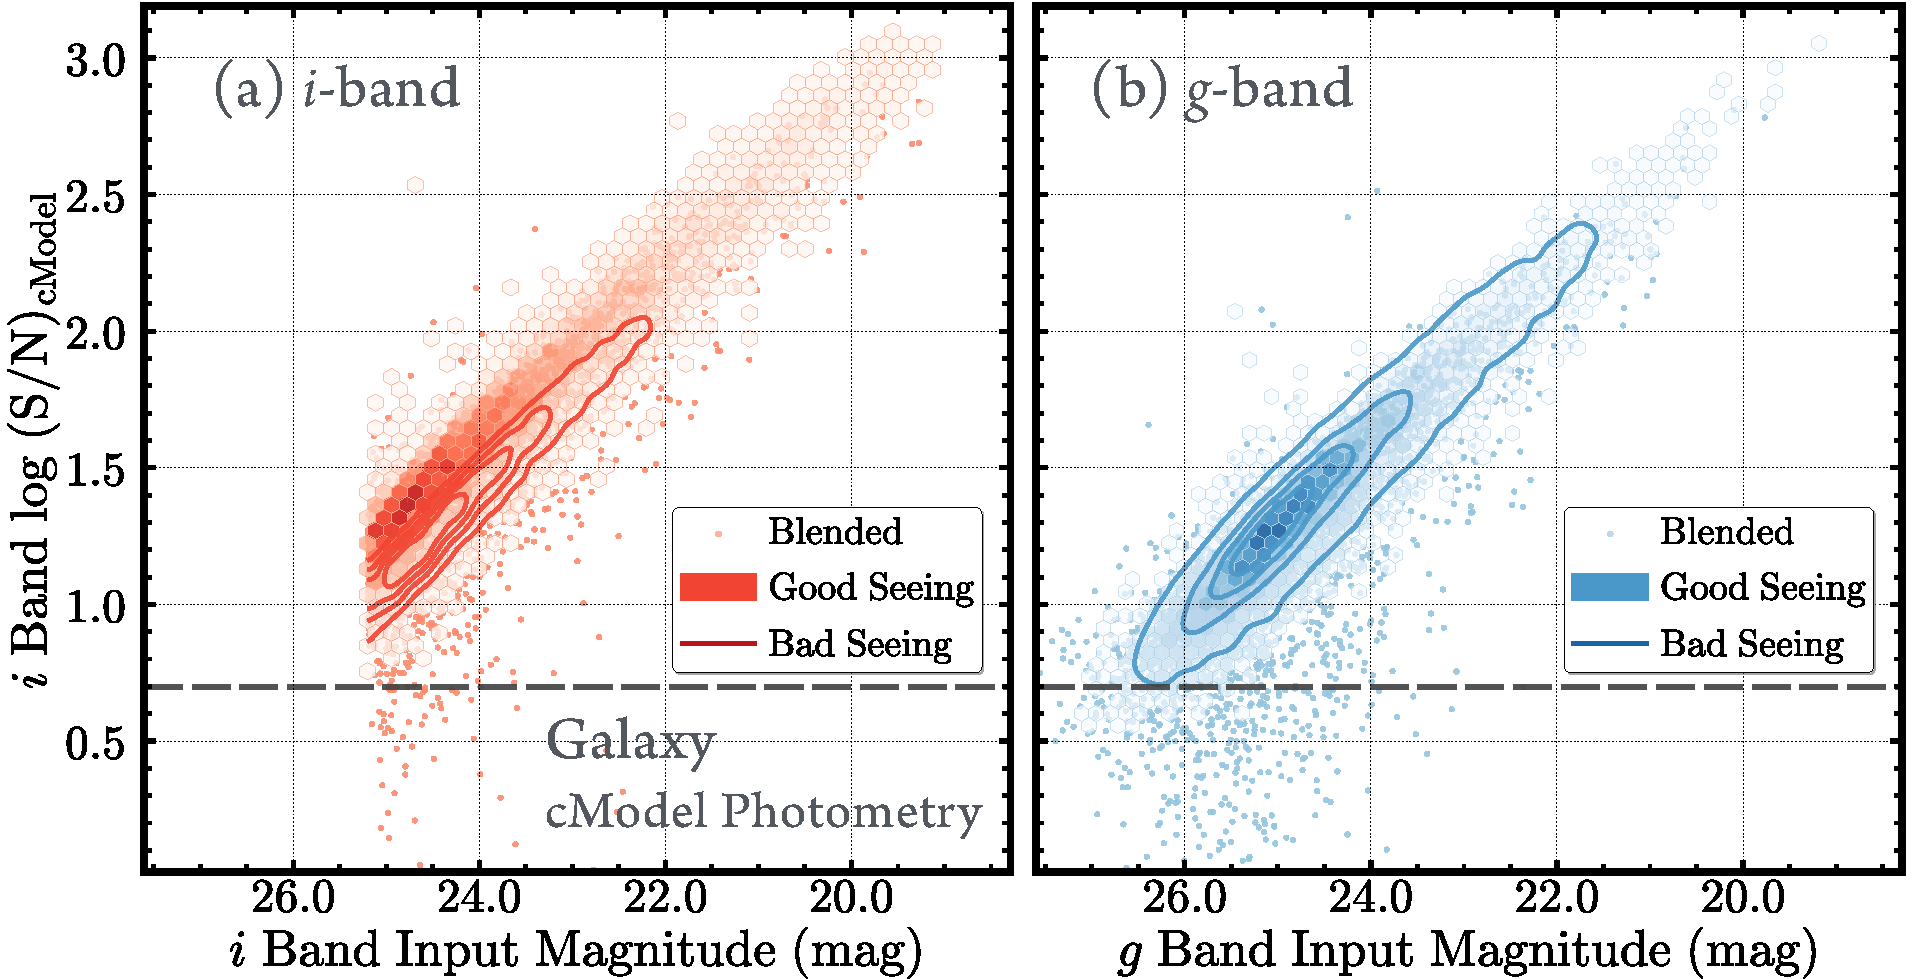
\includegraphics[width=\textwidth]{fig/synpipe_galaxy_sn}
    \end{center}
    \caption{
        Relation between input magnitudes (\textbf{left}: $i$-band; \textbf{right}:
        $g$-band) of synthetic galaxies and the $log(S/N)$ measured by \hscpipe{}
        \cmodel{} photometry.
        The lines and contours legend is similar to Fig \ref{fig:star_sn}
        }
    \label{fig:cmodel_sn}
\end{figure*}
%% ------------------------------------------------------------------------------------ %%

%% ------------------------------------------------------------------------------------ %%
%% Fig: Accuracy of Forced cModel Magnitudes for galaxies
\begin{figure*}
    \begin{center}
        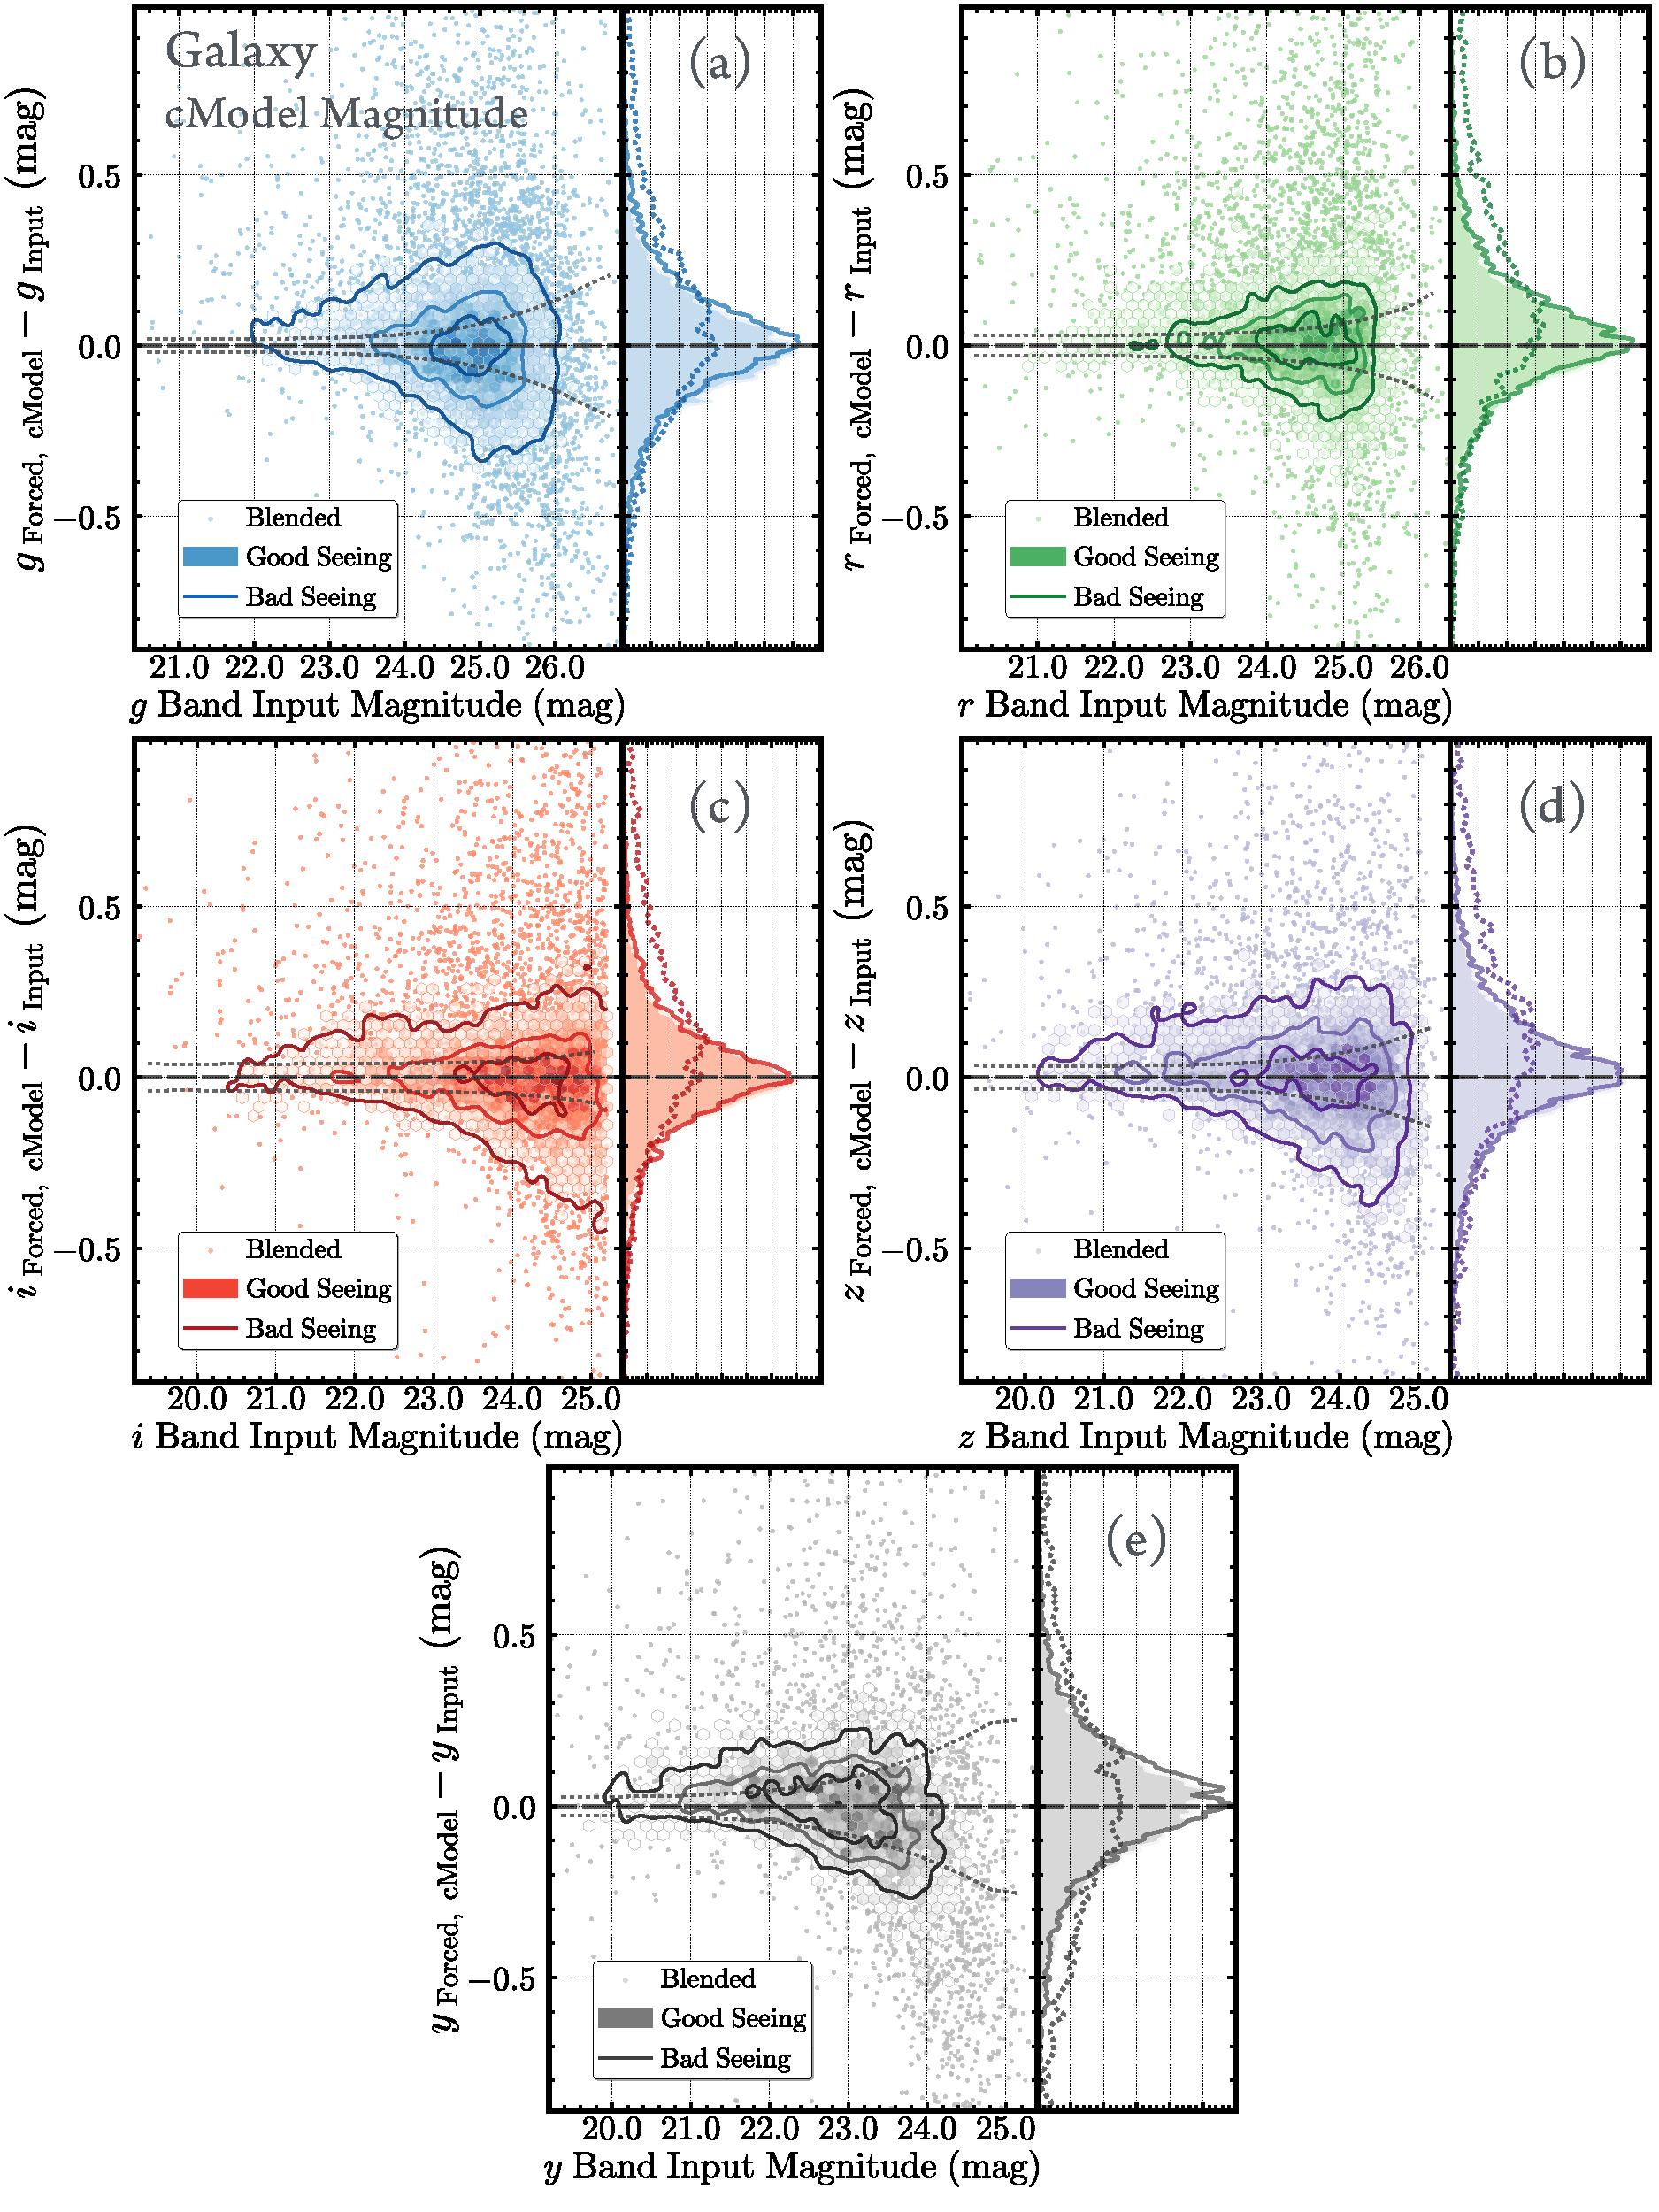
\includegraphics[width=16cm]{fig/synpipe_galaxy_mag}
    \end{center}
    \caption{
        Accuracies of the \texttt{hscpipe} \cmodel{} photometry for synthetic
        galaxies measured by the difference between input and output \forced{}
        \cmodel{} magnitudes.
        Plots [a, b, c, d, e] show the results for [$g$, $r$, $i$, $z$, $y$]-bands, respectively.
       The lines and contours legend is identical to Fig \ref{fig:psf_mag}.
        }
    \label{fig:cmodel_mag}
\end{figure*}
%% ------------------------------------------------------------------------------------ %%

%% ------------------------------------------------------------------------------------ %%
%% Fig: Difference between the Unforced and Forced Magnitudes
\begin{figure*}
    \begin{center}
        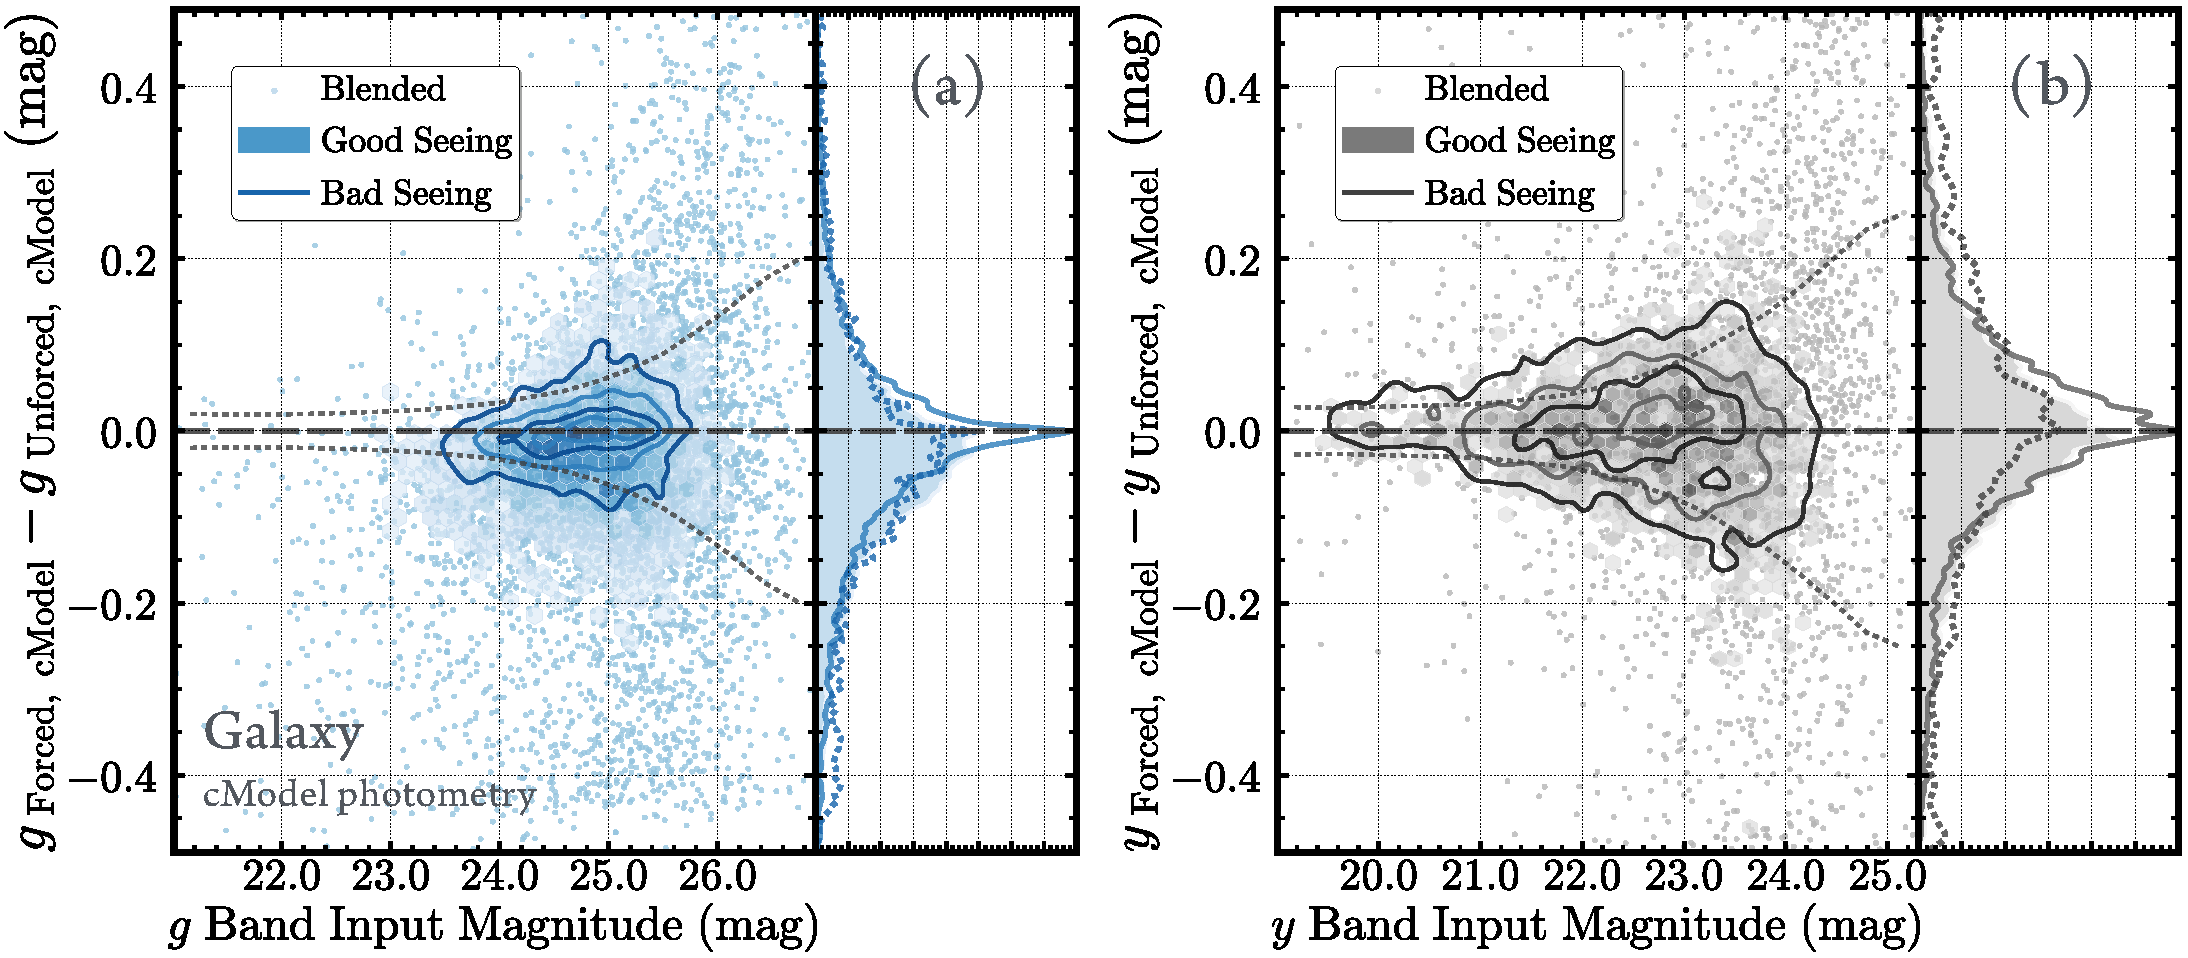
\includegraphics[width=\textwidth]{fig/synpipe_cmodel_diff}
    \end{center}
    \caption{
        The magnitude differences between the \unforced{} and \forced{}
        \cmodel{} photometry for synthetic galaxies in $g$- (\textbf{left} and
        $y$-band (\textbf{right}).
        The lines and contours legend is identical to the plots in Fig \ref{fig:psf_diff}.
        }
    \label{fig:cmodel_diff}
\end{figure*}
%% ------------------------------------------------------------------------------------ %%

%% ------------------------------------------------------------------------------------ %%
%% Fig: Accuracies of the cModel color for galaxies
\begin{figure*}
    \begin{center}
        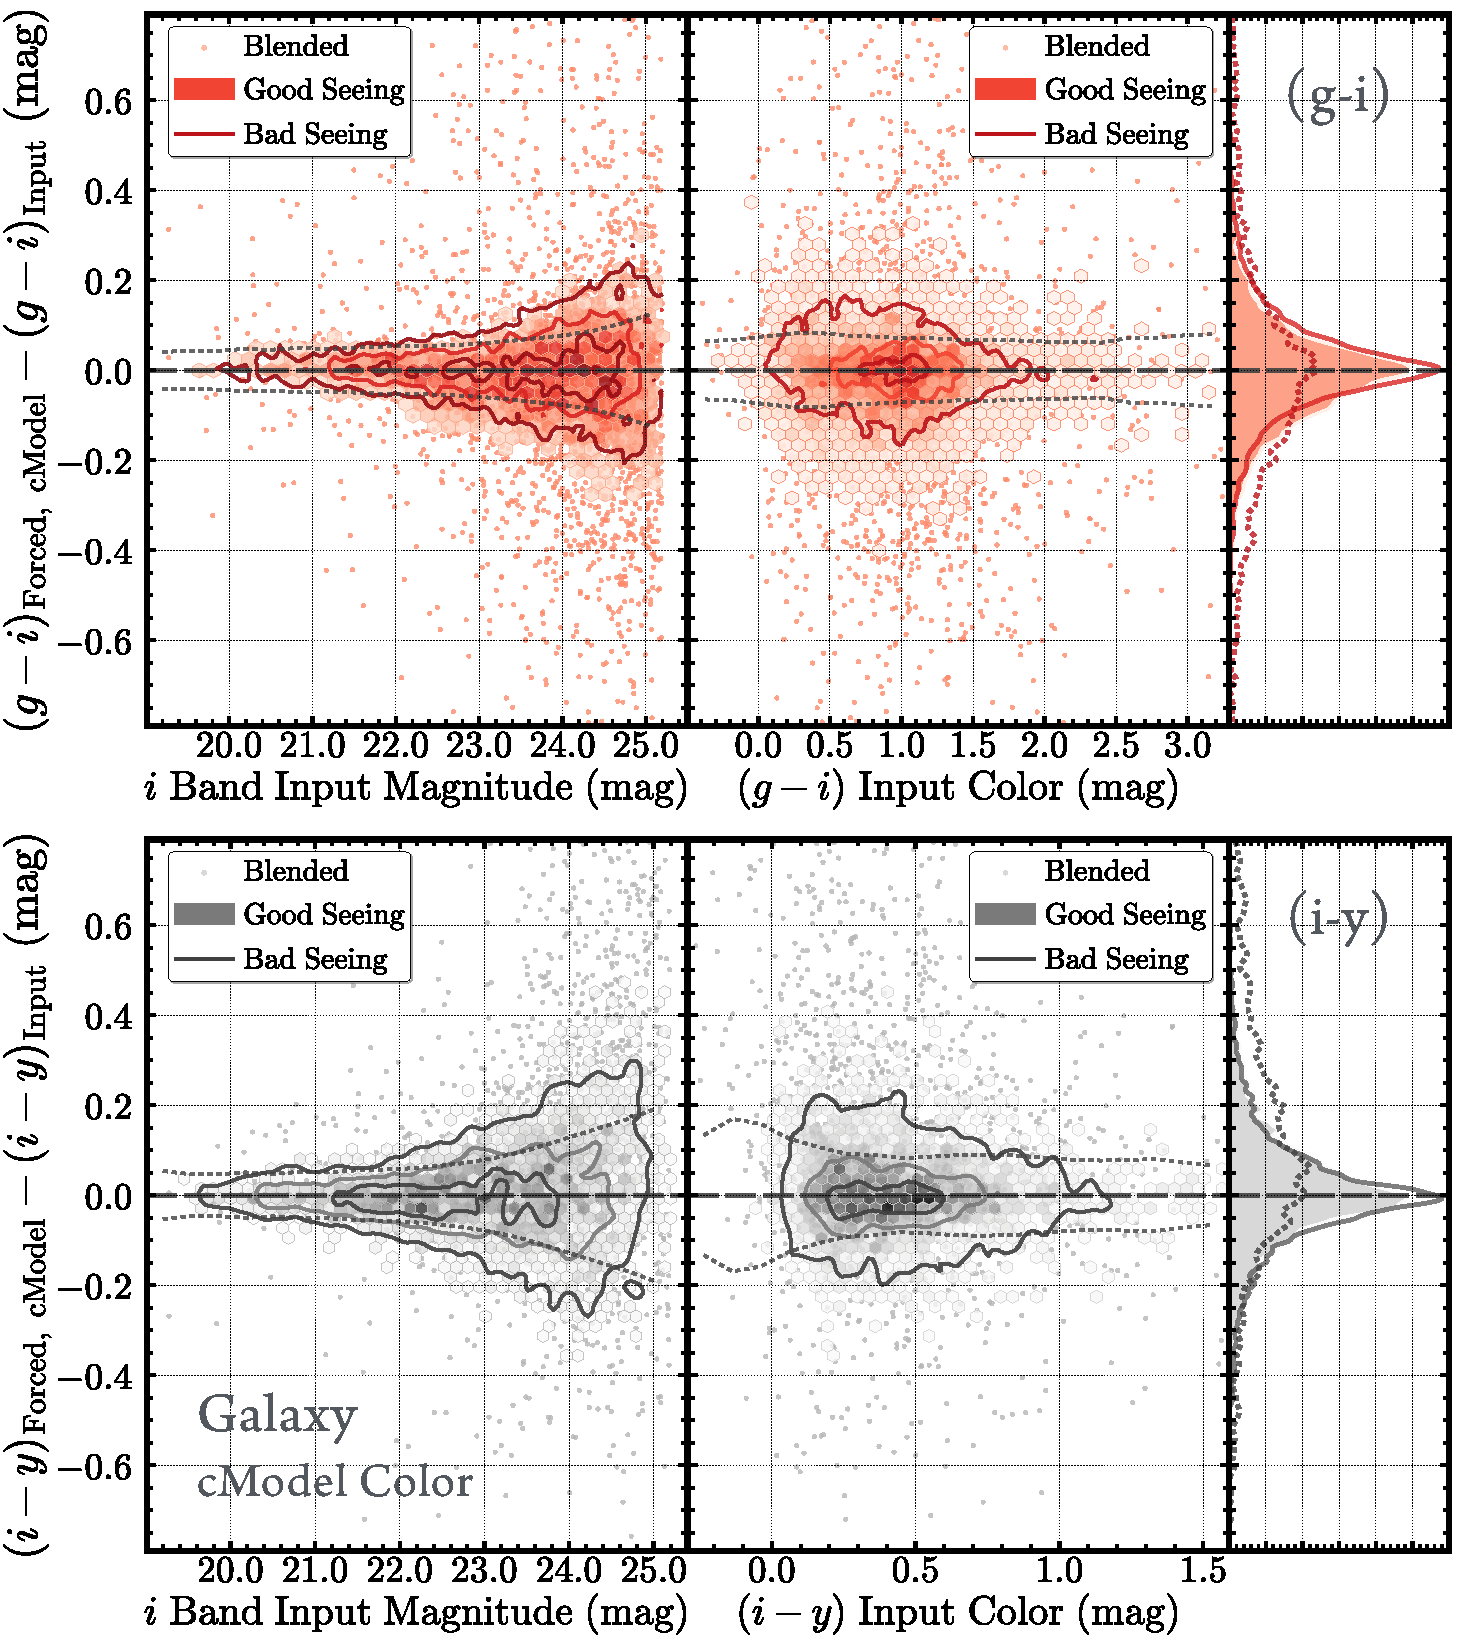
\includegraphics[width=\textwidth]{fig/synpipe_galaxy_color}
    \end{center}
    \caption{
        Accuracies of the color measurements for synthetic galaxies via the
        differences between input and \forced{} \cmodel{} colors.
        The \textbf{upper panels} and \textbf{lower panels} are for $g-i$ and $i-y$
        colors separately.
        The \textbf{left} column shows the relation between input magnitude (x-axis) and
        the color difference, and the \textbf{right} column uses the input colors as
       the  x--axis.
       The lines and contours legend is identical to the plot in Fig \ref{fig:psf_color}.
        }
    \label{fig:cmodel_color}
\end{figure*}
%% ------------------------------------------------------------------------------------ %%

%% ------------------------------------------------------------------------------------ %%
%% Fig: Color-Color Distributions of the Input and Measurements for galaxies
\begin{figure*}
    \begin{center}
        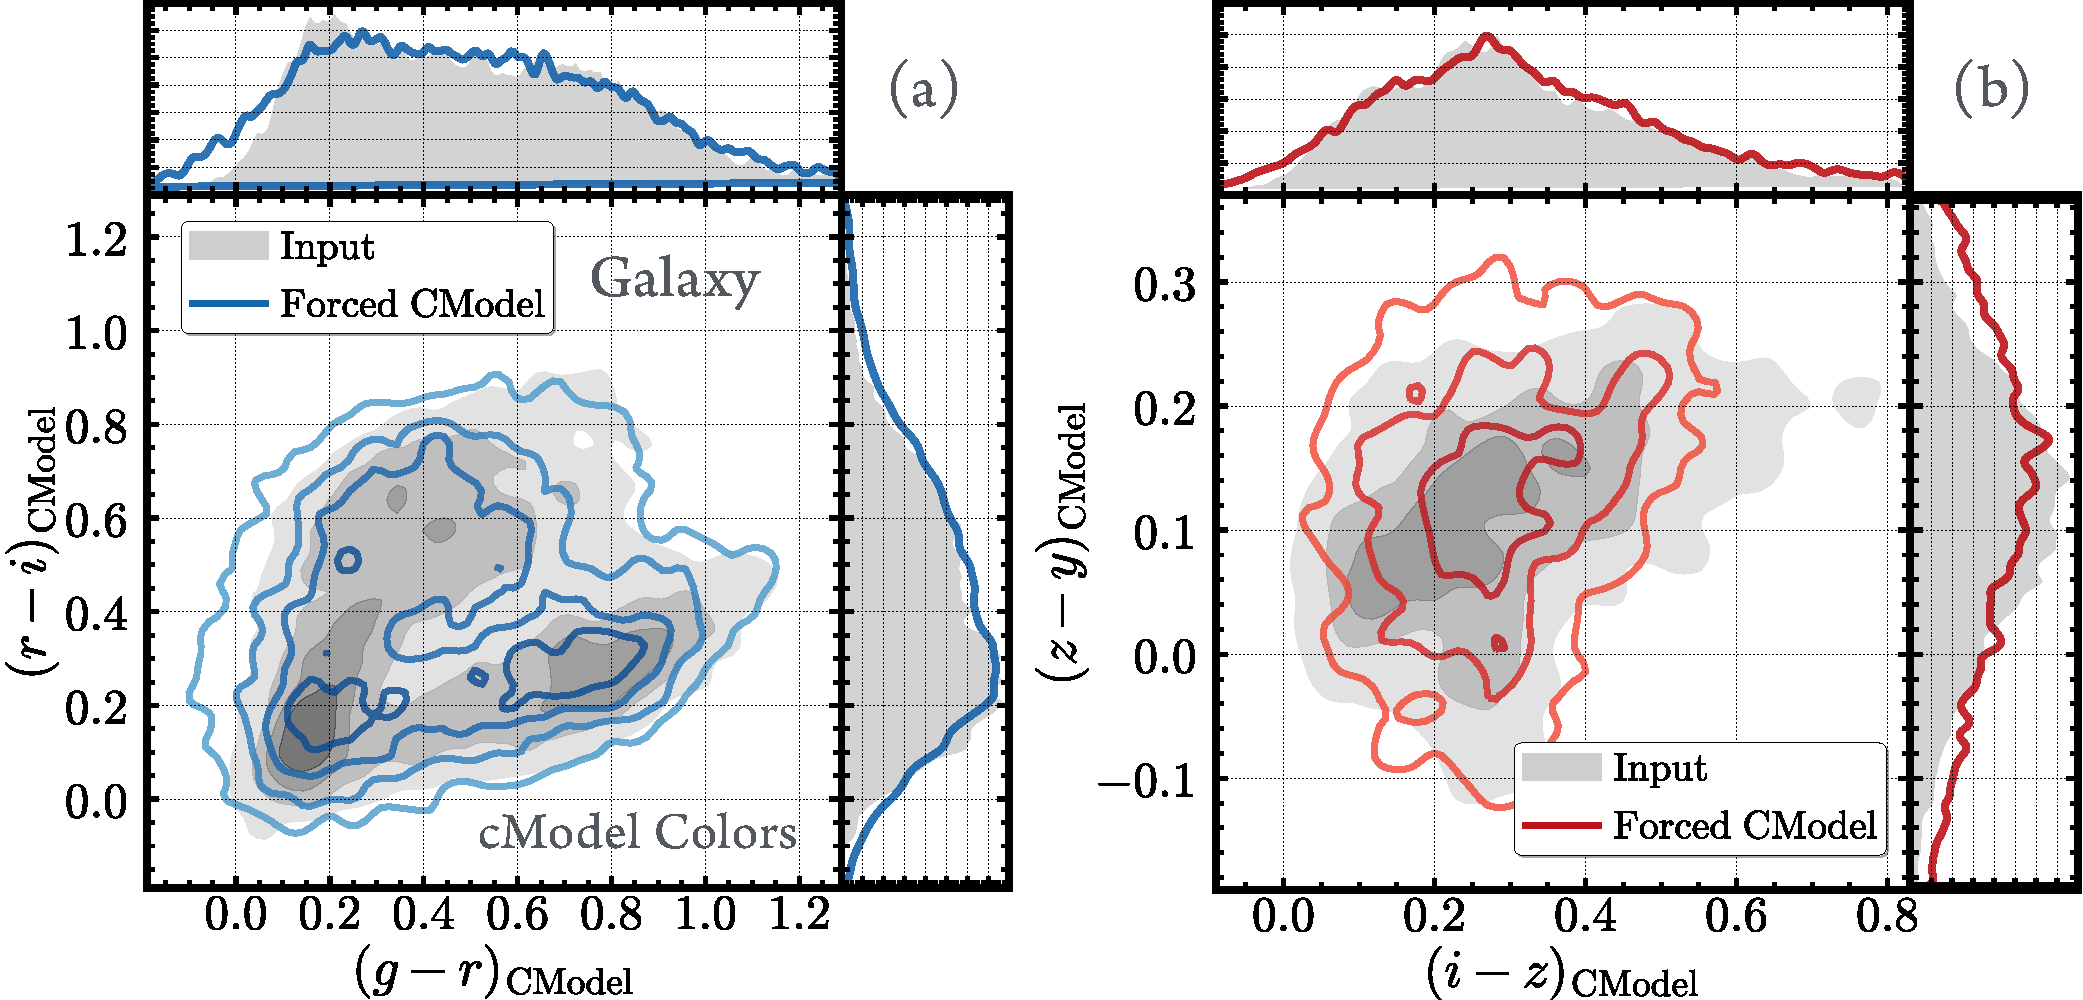
\includegraphics[width=\textwidth]{fig/synpipe_galaxy_cdist}
    \end{center}
    \caption{
        Evaluations of color measurement accuracy for synthetic galaxies
        using the color-color distributions.
        The \textbf{left} panel (a) uses $(g-r)$ vs. $(r-i)$ colors, and the \textbf{right} panel (b)
        uses $(i-z)$ and $(z-y)$ colors.
        The filled contours and shaded histograms reflect the distributions for input
        colors.
        The empty contours and solid-line histograms show the distributions recovered
        by \hscpipe{} \cmodel{} photometry.
        }
    \label{fig:cmodel_cdist}
\end{figure*}
%% ------------------------------------------------------------------------------------ %%

%% ------------------------------------------------------------------------------------ %%
\subsection{cModel photometry of Galaxies}
    \label{ssec:cmodel}

  For galaxies, \hscpipe{} uses a \cmodel{} photometry algorithm
     that is an improved version of the SDSS \cmodel{}
    photometry.
    For more details, please see Bosch\etal (in prep.).
    In short, \cmodel{} tries to fit each object using a combination of de Vaucouleurs
    and exponential profiles that are approximated by multiple Gaussian profiles.
    Despite the limitation of the \cmodel{} method (e.g., sensitive to background
    subtraction and deblender failure), it can deliver robust PSF-corrected fluxes and
    colors for galaxies.

    In our tests, we randomly inject ${\sim}40,000$ synthetic galaxies into each
    \tract{}; and, using an approach similar to that for star selection, we then select galaxy samples for photometric comparisons.
    First, ${\sim}2$--$3$\% of the synthetic galaxies are ambiguously blended with
    real objects, and are hence removed from the sample.
    Among the rest of the sample, ${\sim}2$--$7$\% do not have any match in the
    \synpipe{} results in different \tracts{} and filters.
    The fraction of unmatched objects is slightly higher for the $g$- and $y$-bands.
    For the same filter, the fraction is always higher for the bad-seeing \tract{}.
    The magnitudes of the unmatched galaxies are systematically fainter than the
    matched ones.
    In $i$-band, the median input magnitudes for matched and unmatched galaxies are
    $24.0$ mag and $24.6$ mag, respectively.

    After selecting the matched synthetic galaxies with primary detection and
    clean photometry (see Appendix \ref{app:qc} for details), we have ${\sim}30,000$
    galaxies in each \tract{} for comparison.
   \hscpipe{} misclassifies less than $1$\% of these objects as point sources
    in the good-seeing \tract{}.
    However,   \hscpipe{} misclassifies more objects ($4$\%) in the bad-seeing \tract{}.
    The median input magnitude for these misclassified sources is ${\sim}24.9$ mag
    in $i$-band, significantly fainter than the median of other sources.
    We further discuss this in Section \ref{ssec:sg}.

    We also use $b>0.1$ to define samples of highly blended galaxies.
    Due to the extended nature of the galaxies, the $b$ distributions for synthetic galaxies are
    very different from the  $b$ distributions for synthetic stars, and they also skew toward higher values (especially for the
    bad-seeing \tract{}).
    About $7$--$9$\% of synthetic galaxies are highly blended by this standard.
    The fraction is only slightly higher in the bad-seeing \tract{}, and the
    $g$-band has the highest fraction of highly blended galaxies.
    We highlight the highly blended ones in comparisons, and there are other relevant
    discussions in Section \ref{ssec:blendedness}.

    Although these galaxies span in very wide large ranges of magnitude and
    structural parameters, the majority of them are faint
    ($i_{\mathrm{Input}} > 24.0$ mag) and small ($R_{\mathrm{e}} < 0.5$\asec).
    It is very challenging to obtain good photometric quality of these galaxies, which is crucial
    to achieving several key scientific goals of the HSC survey.
    The selected samples do not provide enough bright or large galaxies to test.
    Therefore, we will supplement results for these galaxies using better samples
    in the future.

%% ------------------------------------------------------------------------------------ %%
\subsubsection{Input magnitude and the \s2n{} of \cmodel{} photometry}

    In Fig \ref{fig:cmodel_sn}, we first show the relation between the input
    magnitudes and the \s2n{} of the synthetic galaxies estimated by the ratio
    between \cmodel{} flux and its uncertainties from \hscpipe{}.
    Since these galaxies are extended objects, the \s2n{} here should be treated
    as the average \s2n{}, which is different from the \s2n{} of stars using PSF
    photometry.

    As we did for stars, we use $i$- and $g$-bands as examples for galaxies.
    The most obvious difference between the  \s2n{} distribution for stars and the  \s2n{} distribution for galaxies is that
    at fixed input magnitude, the galaxy \s2n{} distribution shows much larger
    scatter.
    At the same total flux, a galaxy can have a different size and shape, which
    naturally leads to differences in the galaxy's peak and average \s2n{}.
    This also makes it difficult to have a clear definition of ``detection limit''
    for galaxies.
    For $i$-band, the typical \s2n{} for synthetic galaxies at the magnitude limit
    of our sample ($25.2$ mag) is ${\sim}20$, but at that limit the low-\s2n{} tail has
    reached the \s2n{}$=5$ boundary.
    This suggests that, although HSC Wide can detect galaxies as faint as
    $i{\sim}26.0$ mag, the sample at that magnitude will be significantly incomplete.
    Furthermore, the magnitude limit can also introduce selection bias because galaxies with certain structural properties are harder to detect than others.
    HSC survey data users who want to select flux-limited samples of galaxies,
    or intend to study the population of faint (e.g., high-$z$) galaxies should
    keep this in mind.

    Similar to the synthetic stars, the worse the seeing condition, the more
    we noticed a decrease in \s2n{} at the same magnitude (see Fig \ref{fig:psf_s2n}) 
    for $i$-band).
    Meanwhile, the highly blended synthetic galaxies do not show significantly
    different \s2n{} distributions here.

%% ------------------------------------------------------------------------------------ %%
\subsubsection{Accuracy of the \cmodel{} magnitude}

    In Fig \ref{fig:cmodel_mag}, we illustrate the photometric uncertainties of the
    \cmodel{} magnitudes in each band using the same format as
    Fig \ref{fig:psf_mag}.

    The overall performance of \cmodel{} photometry is very reasonable all the way
    down to $i_{\mathrm{Input}}=25.2$ mag.
    Compared to the qualities of PSF photometry for stars, the magnitude differences
    of \cmodel{} show much larger scatter for galaxies.
    Given the diversity of properties of these galaxies and the complexities in the
    model-fitting process, this difference is expected.
    At the same time, we can see that the \cmodel{} algorithm in \hscpipe{} can
    provide unbiased and consistent photometry for galaxies in different bands and
    seeing conditions.

    In $i$-band, the median flux uncertainty of the \forced{} \cmodel{} is ${\sim}7$\%
    in the good-seeing \tract{} at $i_{\mathrm{Input}}{\sim}20.0$ mag,
    and ${\sim}9$\% at $i_{\mathrm{Input}}{\sim}24.0$ mag.
    Down to $i_{\mathrm{Input}}{\sim}25.0$ mag, the median uncertainty maintains
    at ${\sim}11$\% level.
    For the bad-seeing \tract{} in $i$-band, the performance is very similar.
    From $i_{\mathrm{Input}}{\sim}20.0$ to $25.0$ mag, the median magnitude difference
    between output and input values changes from \plus{}$0.041$ mag to
    \minus{}$0.005$ mag, which suggests that \forced{} \cmodel{} photometry is
    unbiased down to the very faint end.
    It is worth noting that the photometric uncertainties estimated by \synpipe{}
    are significantly larger than the fiducial error from \hscpipe{}, which does not
    take into account the systematic uncertainties involved in the modeling
    fitting process.
    Although the synthetic galaxies in our sample are described by the simple single-\ser{}
    model, the\cmodel{} algorithm can only approximate them to a certain accuracy,
    especially when the noise level, deblending uncertainty, and priors of model
    parameters are considered.
    Given that real galaxies are more complex in structural details, these
    uncertainties should be treated as lower limits.

    The performance of \forced{} \cmodel{} photometry is very consistent across all
    filters.
    For $g$-, $r$-, and $z$-bands, the photometric uncertainties are very similar to
    the ones for $i$-band between $20.0$ and $25.0$ mag.
    The \forced{} \cmodel{} magnitudes are also unbiased for these three filters
    across the entire input magnitude range.
    The uncertainties for $y$-band are slightly larger, ranging from 9\% to 17\% in the
    same magnitude bins.
    In addition, the \forced{} \cmodel{} tends to overestimate the total flux in $y$-band
    at $y_{\mathrm{Input}}>24.0$ mag.
    Mean magnitude differences change from \minus{}0.06 at 24.0 mag to \minus{}0.22
    mag at 25.0 mag.
    Both a worse seeing condition and a higher background noise level can make it more
    difficult to detect a faint object on a $y$-band image.
    At $y_{\mathrm{Input}}{\sim}24.0$, the average \s2n{} for \cmodel{} in $y$-band
    is already close to the detection threshold.

    As mentioned, the statistics for brighter galaxies are very uncertain due to the
    small sample size.
    However, we do notice that, at $i_{\mathrm{Input}}<20.0$, the \forced{}
    \cmodel{} photometry shows larger uncertainty and starts to systematically
    underestimate the total flux.
    This problem is confirmed via comparing with more carefully derived total fluxes
    for bright galaxies (e.g., \citealt{HSCDR1}, Huang\etal in prep.).
    It relates to the known issues of \hscpipe{} (e.g., \hscpipe{}over-deblends around bright objects; inappropriately weights priors in \cmodel{}); but it may also suggest
    that, at the imaging depth of HSC, assumptions in \cmodel{} are no longer the
    best choice in modeling these galaxies (e.g., for massive elliptical galaxies;
    see Huang\etal in prep.~for more details).

    For the highly blended synthetic galaxies, we also see systematically
    underestimated total flux (average offset ${\sim}0.1$ mag) and larger scatter
    of photometric uncertainty in all five bands.
    Meanwhile, the contrast between relatively isolated and highly blended galaxies
    in photometric performance is not as staggering as the one for synthetic
    stars (Fig \ref{fig:psf_mag}).

    We also test the \unforced{} \cmodel{} photometry in all five bands, and the
    results suggest similar accuracies.
    We highlight the differences between \forced{} and \unforced{} \cmodel{}
    photometry in $g$- and $y$-bands in Fig \ref{fig:cmodel_diff}.
    The only noticeable difference is for galaxies brighter than $24.0$ mag in
    $g$-band; their \forced{} \cmodel{} magnitudes are systematically brighter than
    the \unforced{} ones.

%% ------------------------------------------------------------------------------------ %%
\subsubsection{Accuracy of the \cmodel{} color}

    The consistent and accurate five-band \cmodel{} colors from \hscpipe{} are crucial
    to the photometric redshift and spectral energy distribution (SED) fitting results.
    They are also key to the selection of high-$z$ Lyman-break galaxies (LBG) and
    and many other interesting objects.

    In Fig \ref{fig:cmodel_color}, we demonstrate the accuracies of \forced{} $(g-i)$
    and $(i-y)$ \cmodel{} colors in the same format used for synthetic stars
    (Fig \ref{fig:psf_color}).
    These plots show that \hscpipe{} can provide reliable \cmodel{} colors for
    synthetic galaxies down to $i_{\mathrm{Input}}{\sim}25.0$ mag.
    For $(g-i)$ colors, the average uncertainty around $i_{\mathrm{Input}}{\sim}21.0$ mag
    is ${\sim}0.04$ mag.
    The uncertainty increases to ${\sim}0.11$ mag at $i_{\mathrm{Input}}{\sim}25.0$ mag.
    Results for $(i-y)$ colors are similar.

    The performance of \forced{} \cmodel{} color does not show dependence on seeing
    condition, and it is unbiased across the ranges for input total magnitude and color.
    The only noticeable feature is that the $(i-y)$ color at
    $i_{\mathrm{Input}}>24.0$ is slightly overestimated.
    As mentioned above, this is not surprising given the shallower imaging depth of  the
    $y$-band.
    At the same time, high blendedness of synthetic galaxies can still increase the
   color uncertainties and bias the color measurements.
    The highly blended galaxies on average show slightly bluer  $(g-i)$ colors
     and redder  $(i-y)$ colors  than the input values.

    Similar to the star comparison in Fig \ref{fig:psf_cdist}, we also compare the color--color distributions
    of the input and output \forced{} \cmodel{} values in Fig \ref{fig:cmodel_cdist}.
    The general color distributions are well recovered despite the fact that the galaxy accuracy is
    not as good as the accuracy for stars, especially on the $(i-z)$ vs. $(z-y)$ plane.
    That result is expected given the narrow dynamical ranges of these colors among red filters.
    The \forced{} \cmodel{} tends to slightly underestimate the $(g-r)$ and $(i-z)$
    colors at the very ``blue'' end, while overestimating the $(i-y)$ color at the very
    red end.

   We should point out that we assume constant color for the entire galaxy.
    In reality, different colors for individual components and a smooth color gradient
    can complicate the situation; hence, the uncertainties of \cmodel{} colors
    here should be considered as lower limits.
%% ------------------------------------------------------------------------------------ %%


%% ------------------------------------------------------------------------------------ %%
%% Fig: Astrometric Calibration
\begin{figure*}
    \begin{center}
        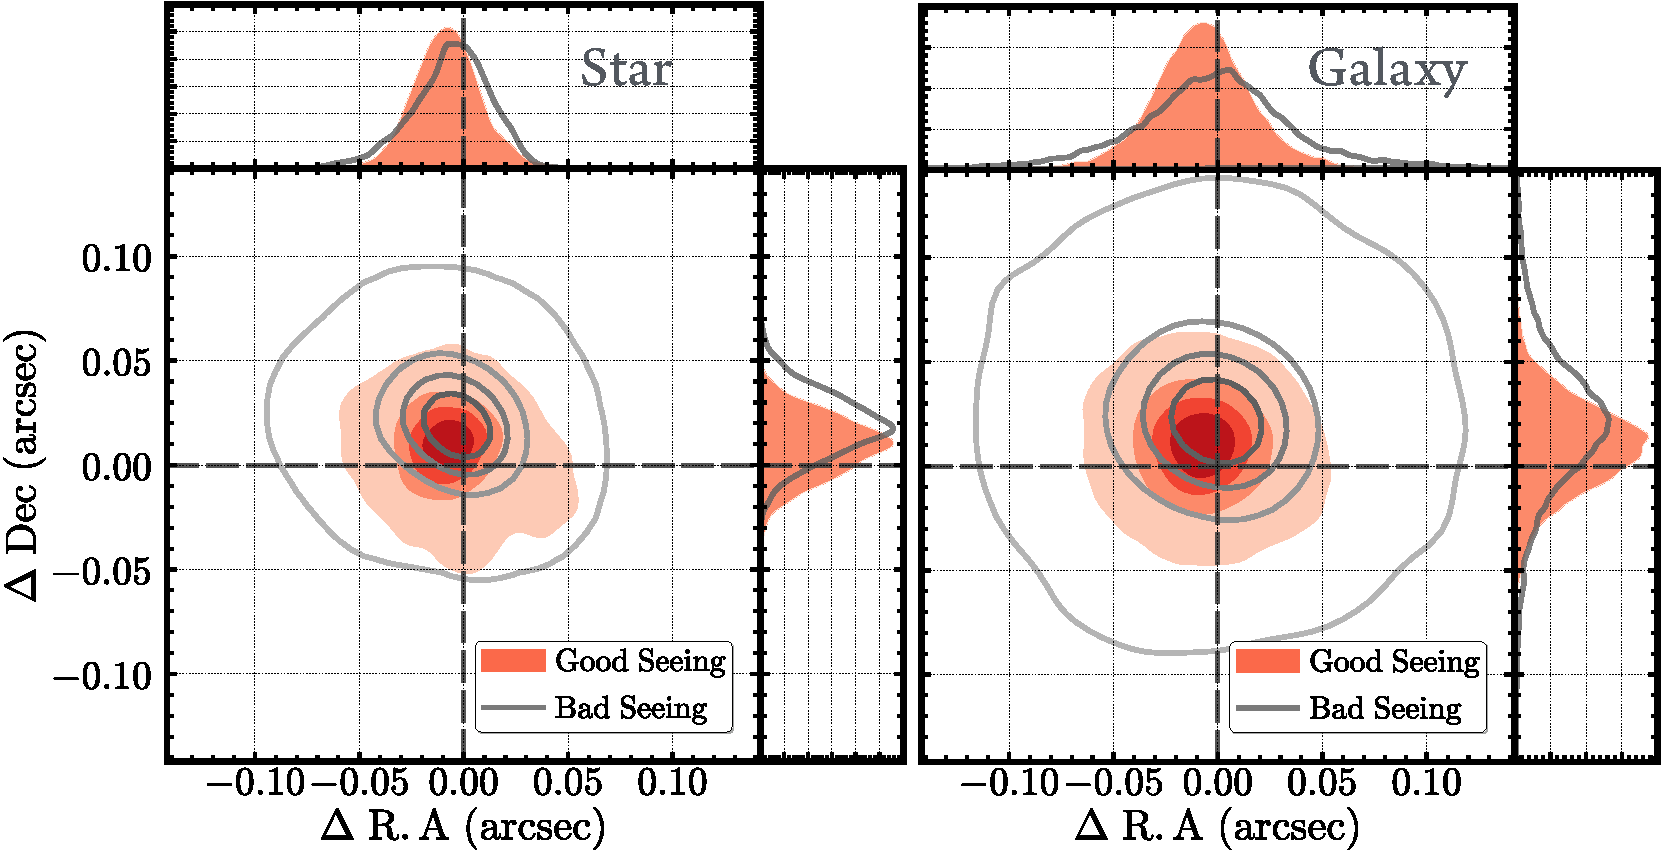
\includegraphics[width=\textwidth]{fig/synpipe_astrometry}
    \end{center}
    \caption{
        Astrometric accuracy for a synthetic star (\textbf{left}) and a galaxy
        (\textbf{right}) via the differences in R.A and Dec between the input
        coordinates and the ones measured on the \coadd{} images.
        Hexagonal bins (filled histogram) and contours (solid-line histogram) are for
        the synthetic objects from \tracts{} with good and bad seeing conditions, respectively.
        $\Delta\mathrm{R.A}=0$ and $\Delta\mathrm{Dec}=0$ are marked by dashed lines.
        }
    \label{fig:astrometry}
\end{figure*}
%% ------------------------------------------------------------------------------------ %%


%% ------------------------------------------------------------------------------------ %%
%% Fig: Star-Galaxy Separation
\begin{figure*}
    \begin{center}
        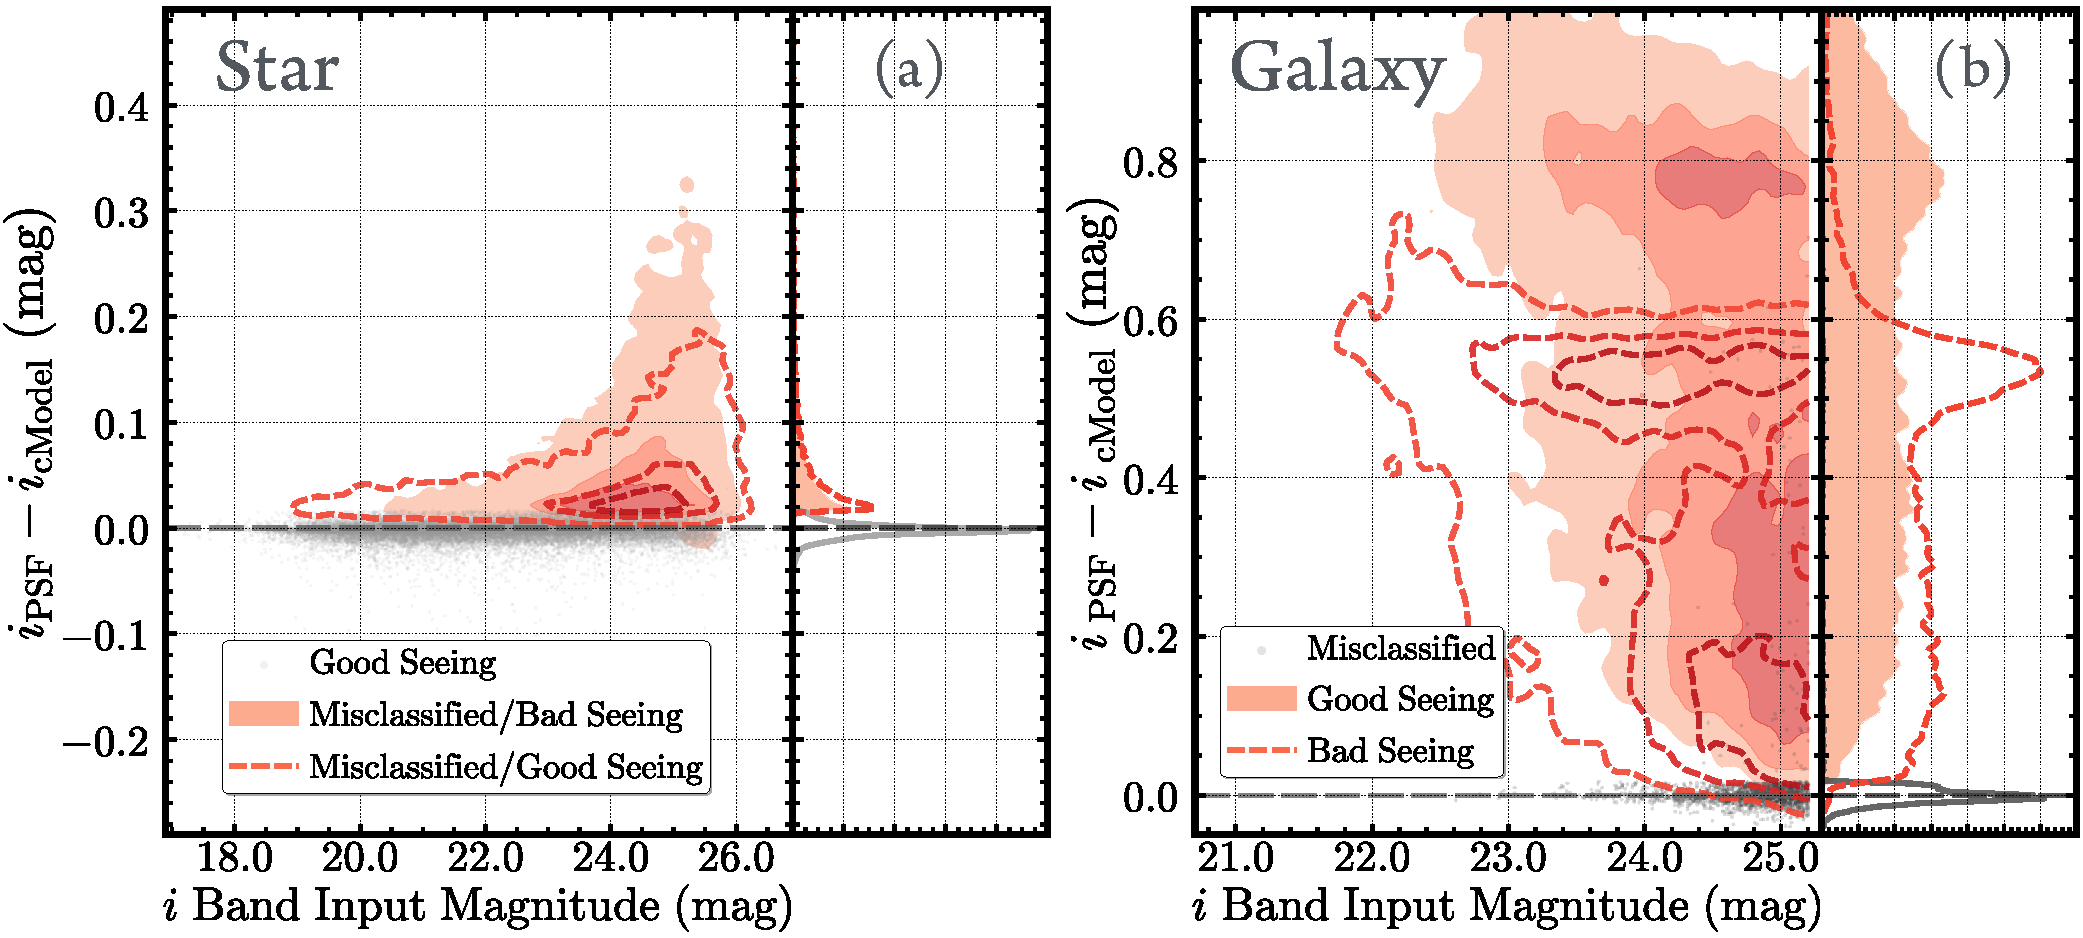
\includegraphics[width=\textwidth]{fig/synpipe_star_galaxy}
    \end{center}
    \caption{
        Problems with the current  \hscpipe{}star--galaxy separation method, which is based on the magnitude difference between the PSF and
        \cmodel{} photometry.
       The plot on the \textbf{left} (a) illustrates distributions for the synthetic stars.
        Hexagonal bins and filled histogram show distributions of correctly classified
        synthetic stars in the good-seeing \tract{}.
        The scatter plot (dashed-line histogram) and contour (solid-line histogram)
        show distributions of synthetic stars that are misclassified as extended
        objects in \tracts{} with bad and good seeing conditions, respectively.
        The plot on the \textbf{right} (b) illustrates distributions for synthetic galaxies.
        Hexagonal bins (filled histogram) and contours (solid-line histogram)
        are for galaxies from good- and bad-seeing \tracts{}, respectively.
        The scatter plot and dashed-line histogram are for synthetic galaxies that are
        misclassified as point sources.
        Zero magnitude difference is highlighted using dashed lines on both plots.
        }
    \label{fig:sg}
\end{figure*}
%% ------------------------------------------------------------------------------------ %%

%% ------------------------------------------------------------------------------------ %%
%% Fig: Relations between Blendedness and Photomertic Errors
\begin{figure*}
    \begin{center}
        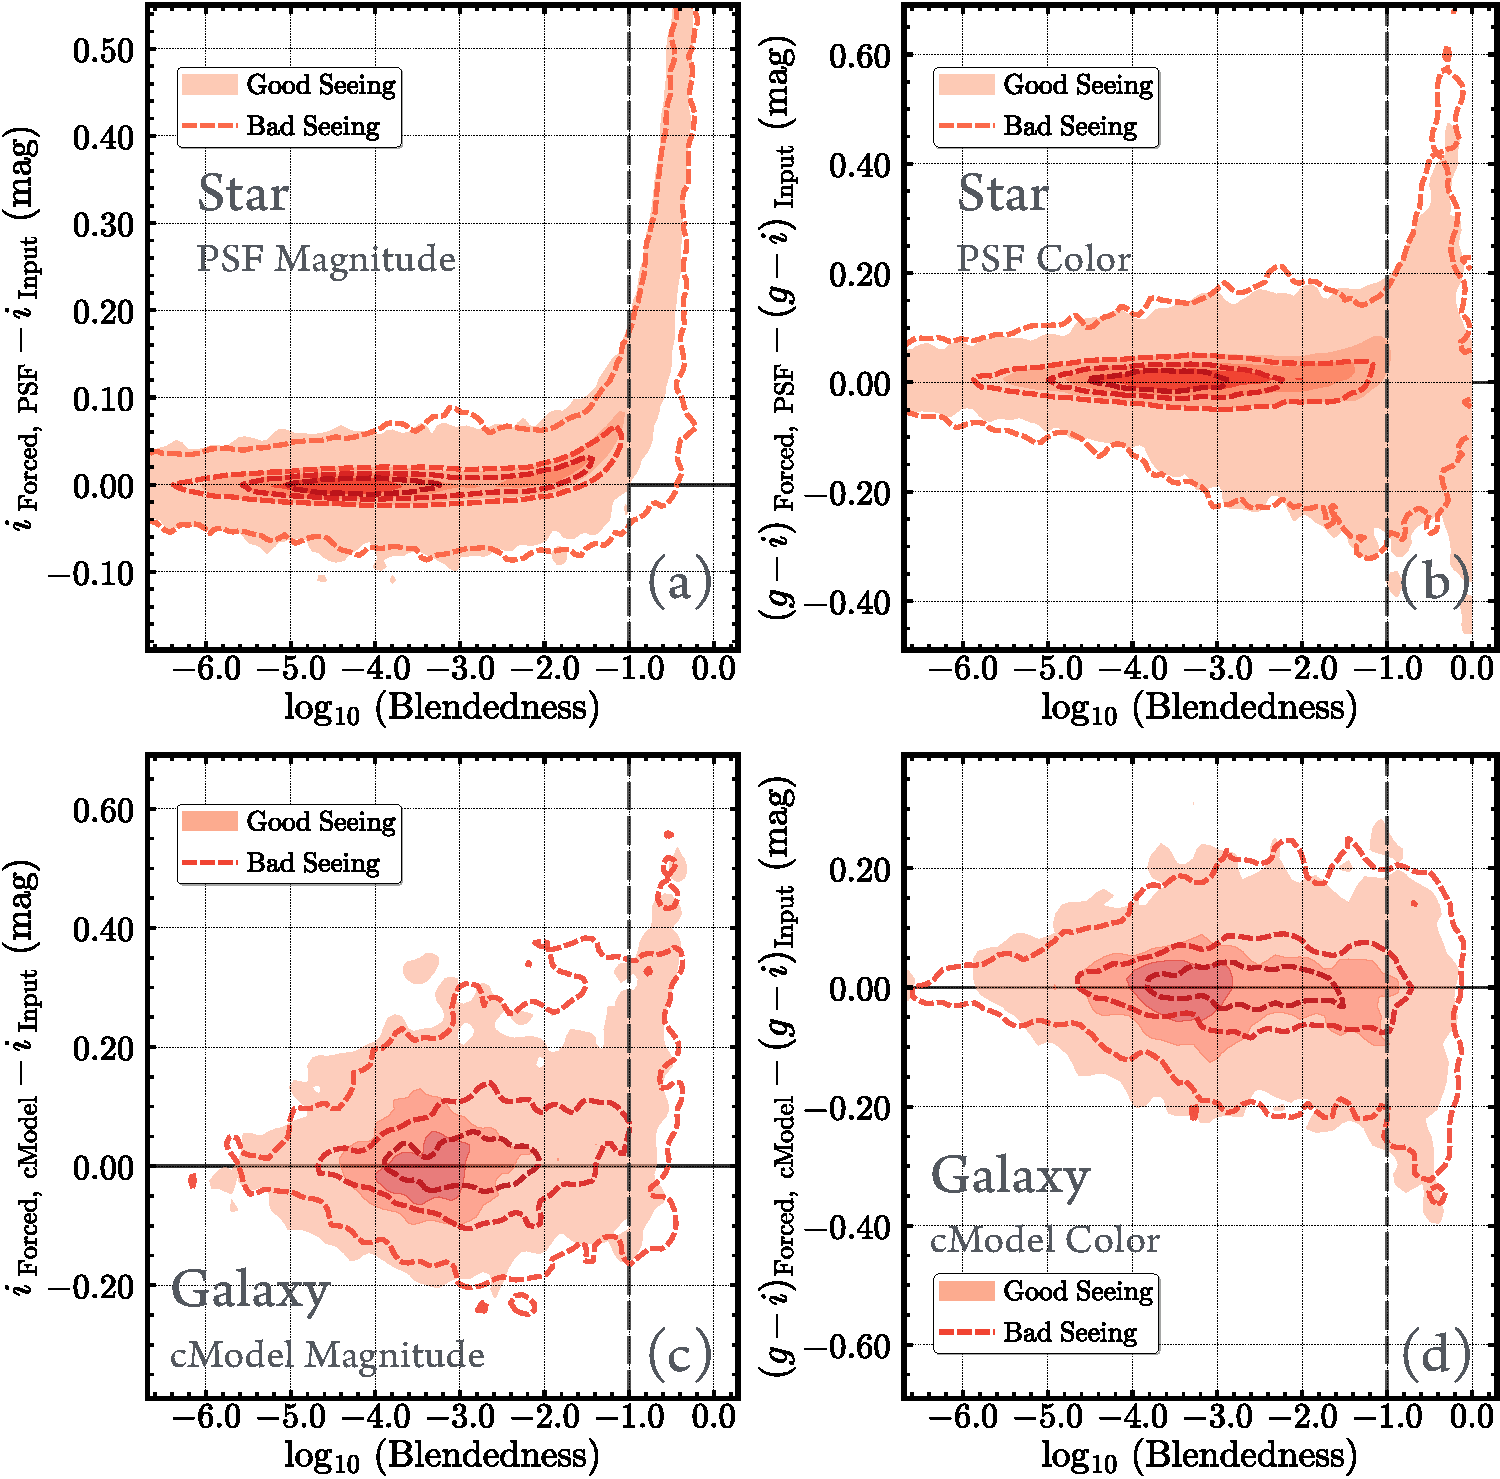
\includegraphics[width=\textwidth]{fig/synpipe_blendedness_err}
    \end{center}
    \caption{
        The relation between the $\log(\mathrm{Blendedness})$ parameter
        and the photometric accuracies for synthetic stars (\textbf{upper row}, a and b) and
        galaxies (\textbf{lower row}, c and d) .
       The \textbf{left} column (a and c) is for uncertainties of PSF or \cmodel{} magnitude,
        and the \textbf{right} column (b and d) is for uncertainties of $(g-i)$ color.
        Hexagonal bins and contours show results for good- and bad-seeing
        \tracts{}, respectively.
        $\log(\mathrm{Blendedness}) = -1.0$ is marked using a vertical dashed line.
        }
    \label{fig:blend}
\end{figure*}
%% ------------------------------------------------------------------------------------ %%

%% ------------------------------------------------------------------------------------ %%
%% Fig: Compare with the behaviours of the Kron photometry for galaxies
%\begin{figure*}
%    \begin{center}
%        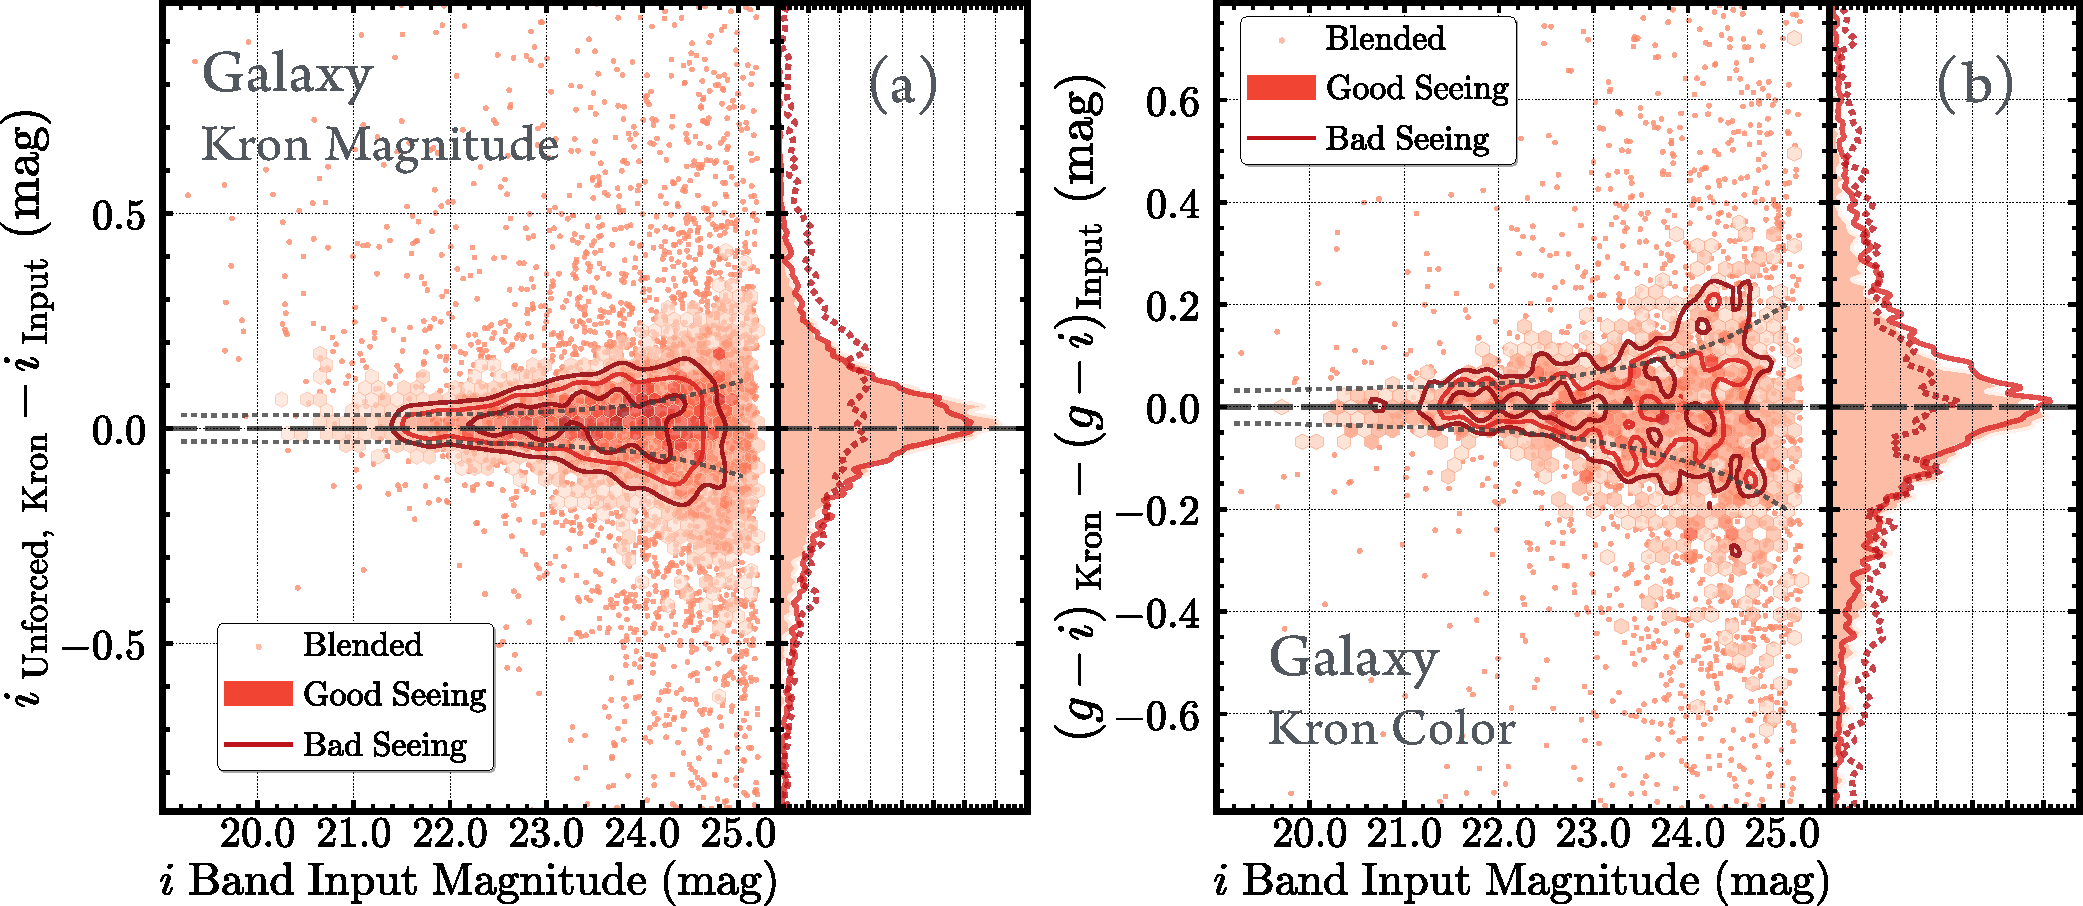
\includegraphics[width=\textwidth]{fig/synpipe_galaxy_kron}
%    \end{center}
%    \caption{
%        Basic performance of the Kron photometry for synthetic galaxies.
%        \textbf{Left} shows the accuracy in $i$-band.
%        magnitude. The format is identical to Fig \ref{fig:galaxy_mag}.
%        \textbf{Right} shows the accuracy of the $(g-i)$ color using
%        Kron photometry.
%        Other formats are identical to Fig \ref{fig:cmodel_color}.
%        }
%    \label{fig:galaxy_kron}
%\end{figure*}
%% ------------------------------------------------------------------------------------ %%

%% ------------------------------------------------------------------------------------ %%
%% Fig: HSC cModel has problem recovering the size and shape of galaxies
\begin{figure*}
    \begin{center}
        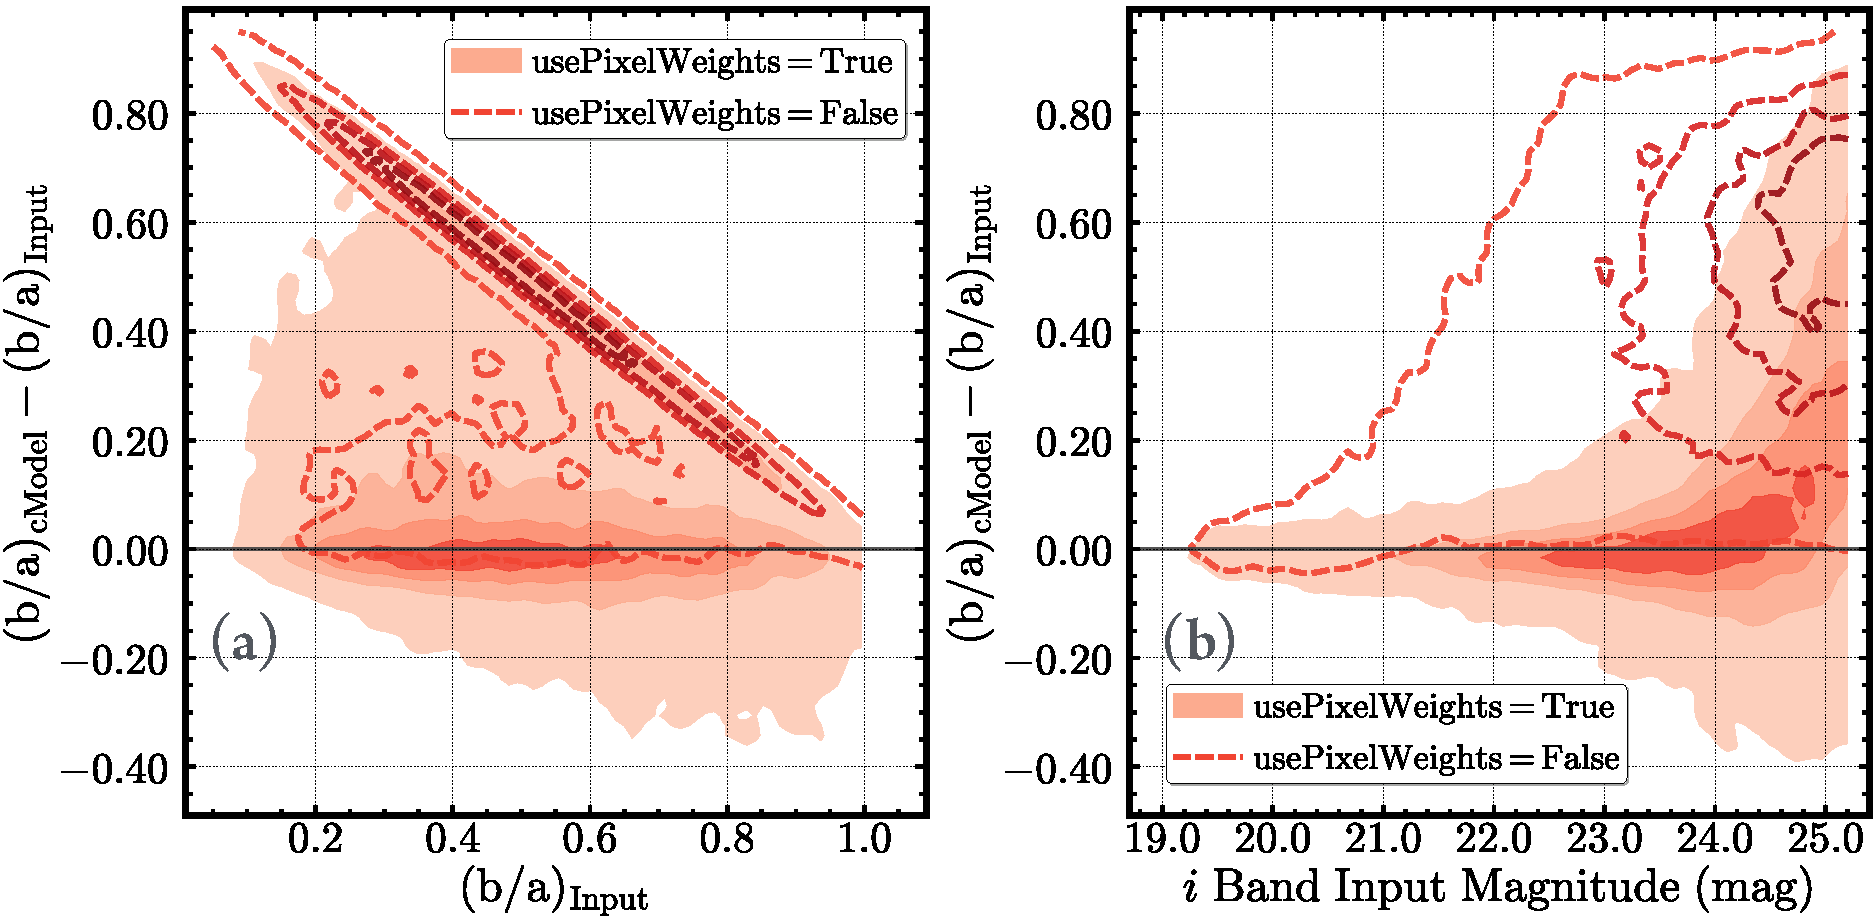
\includegraphics[width=\textwidth]{fig/synpipe_galaxy_ba}
    \end{center}
    \caption{
        Accuracy of the weighted axis ratio measurements for synthetic
        galaxies using \cmodel{} photometry.
      The  \textbf{left} (a) plot shows the relation between the input $(b/a)$ and the
        uncertainties of $(b/a)$ estimates.
        The \textbf{right} (b) plot shows the relation between input magnitude of a synthetic galaxy
        and the $(b/a)$ uncertainties.
        Contours are for the default test with \texttt{usePixelWeights=False}, and the
        hexagonal bins are used for same tests with \texttt{usePixelWeights=True}.
        }
    \label{fig:galaxy_ba}
\end{figure*}
%% ------------------------------------------------------------------------------------ %%


%% ------------------------------------------------------------------------------------ %%

\section{Results on Other Aspects of \hscpipe{}}
    \label{sec:others}

    In this section, we briefly discuss a few other  \hscpipe{} aspects that relate
    to astrometric calibration, star-galaxy separation, blendedness and photometric errors, and galaxy shape measurements to demonstrate the range of topics that can be tested with \synpipe{}.

%% ------------------------------------------------------------------------------------ %%
\subsection{Astrometric Calibration}
    \label{ssec:astrometry}

    For a \synpipe{} test, we inject synthetic objects to single-\visit{} images using
    the less accurate initial astrometric calibration.
    During the image stacking step, the joint calibration process  improves the
    astrometric solutions.
    Therefore, the differences between the input and output coordinates from \synpipe{}
    can help us understand the systematic effect of the image stacking step.

    In Fig \ref{fig:astrometry}, we plot the distributions of astrometric offsets for
    both synthetic stars and galaxies in good- and bad-seeing \tracts{}.
    Small systematic offsets at ${\sim}10$--20 mas can be noticed in either direction.
    The two \tracts{} apparently show different systematic offsets.
    In the same \tracts{}, synthetic stars and galaxies show very similar offsets,
    although the scatter for galaxies is slightly larger due to their extended nature.

%% ------------------------------------------------------------------------------------ %%
\subsection{Star-Galaxy Separation}
    \label{ssec:sg}

    Star--galaxy separation is an important aspect of a cosmology survey,
    and it becomes increasingly difficult at very faint magnitude ($i<24.0$ mag).
    In \hscpipe{}, the star--galaxy classification primarily depends on the extendedness
    value, which is measured by the magnitude difference between PSF and \cmodel{}
    photometry in $i$-band.
    For more details about this algorithm, please see Bosch\etal
    (in prep.).

    In Fig \ref{fig:sg}, we show the current status of star--galaxy classification
    via comparing the input magnitude with the difference between PSF and \cmodel{}
    magnitudes for both synthetic stars and galaxies, and we highlight the distributions
    for misclassified objects.
    As described above, more than $20$\% of synthetic stars at
    $i_{\mathrm{Input}}>23.0$ mag are misclassified as extended objects, while only a
    tiny fraction of faint synthetic galaxies ($i_{\mathrm{Input}}>24.0$) are
    misclassified.
    This confirms that the current star--galaxy classification strategy in \hscpipe{}
    results in a galaxy sample with \textbf{high completeness} and star sample
    with \textbf{high purity}.

    It is also clear that seeing condition strongly modifies the distributions
    of $i_{\mathrm{PSF}}-i_{\mathrm{cModel}}$, where worse seeing conditions clearly make it
    more difficult to separate star and galaxy.
    This implies that the completeness or purity of the galaxy or star sample at the faint end may depend on seeing; therefore, seeing condition deserves the attention of HSC users who care about these properties.

    In the next data release, \hscpipe{} will include a better star--galaxy classifier, which will be based on a machine learning method that takes shape and color information into account. We will test its improvement using \synpipe{} in the future.

%% ------------------------------------------------------------------------------------ %%
\subsection{Blendedness and Photometric Errors}
    \label{ssec:blendedness}

    In the above sections, we have pointed out the impact of high blendedness on
    photometry through a small sample of highly blended objects.
    Here, in Fig \ref{fig:blend}, we further explore the effect of blendedness via
    directly plotting it against the uncertainties of magnitudes and colors.

    For both PSF and \cmodel{} magnitude distributions, we can see clear trends that total fluxes are systematically underestimated for highly blended
    ($b>0.05$ for stars or $0.1$ for galaxies) objects.
    This effect is particularly strong for stars.
    As for colors, higher blendedness still results in higher uncertainties for both
    stars and galaxies, but the trends are different for each.
    Highly blended stars have clearly overestimated $(g-i)$ colors, and the
    highly blended galaxies seem to have  $(g-i)$ colors that are bluer than the true values.

    These blendedness-related uncertainties are not included in the photometric errors released by \hscpipe{}.
    We therefore remind the HSC users to treat the highly blended object with
    greater caution.

%% ------------------------------------------------------------------------------------ %%
%\subsection{Comparing to Kron photometry}

%    \plan{Uses $i$-band as example to briefly discuss Kron photometry}

%    \plan{Although magnitude for galaxies is Ok, the color becomes worse}

%% ------------------------------------------------------------------------------------ %%
\subsection{Shape and Structural Parameters of Galaxies}
    \label{ssec:shape}

    In SDSS,  structural parameters like size and shape from \cmodel{} are often
    used to study the evolution galaxies.
    Although the \cmodel{} in \hscpipe{} follows a very similar algorithm, its primary
    goal now is to provide accurate and consistent magnitude and color in all five
    HSC filters for a vast majority of faint, small galaxies.
    To improve the stability of \cmodel{} for these low-\s2n{} and barely resolved
    galaxies, \hscpipe{} uses Bayesian priors on a radius and axis ratio that strongly
    favors these galaxies.
    However, the current implementation of these priors has a flaw that leads to
    severely underestimated size and overestimated axis ratio for most galaxies.

    In Fig \ref{fig:galaxy_ba}, we demonstrate this issue using the difference between
    the \cmodel{} axis ratio and the input values as an example.
    Here, $({\mathrm{b}/\mathrm{a}})_{\mathrm{CModel}}$ is a combination of the
    axis ratios estimated by the exponential and de Vaucouleurs models weighted by their flux ratio.

    During the investigation, we noticed that one of the problems relates to the \cmodel{} \texttt{usePixelWeight} configuration, which decides whether to
    use per-pixel variances as weights in the nonlinear fit.
    By default, \hscpipe{} chooses \texttt{usePixelWeight}$=$\texttt{False}.
    As one can see, this leads to a significantly overestimated axis ratio for almost
    all galaxies with $i_{\mathrm{Input}}>21.5$ mag\footnote{It also leads to an
    underestimated half-light radius for these galaxies.}.
    At the same time, we also repeat the \synpipe{} run for galaxies with
    \texttt{usePixelWeight}$=$\texttt{True}, and this change clearly mitigates
    the problem. When we use \texttt{usePixelWeight}$=$\texttt{True},
     $({\mathrm{b}/\mathrm{a}})_{\mathrm{CModel}}$ can provide an unbiased axis ratio estimation
    for galaxies with $i_{\mathrm{Input}}< 24.0$ mag.

    For the current HSC data release, we warn users against using the \cmodel{}
    size and shape to study a galaxy with $i_{\mathrm{Input}}>21.5$.
    At the same time, \synpipe{} will try to help \hscpipe{} improve the details
    of the \cmodel{} so that it can provide more useful structural information without hurting its photometric performance.

%% ------------------------------------------------------------------------------------ %%

%% ------------------------------------------------------------------------------------ %%
\section{Summary and Conclusion}
    \label{sec:summary}

    %% Short summary
    In February 2017, the HSC survey made its first public data release, and the survey continues to
    produce increasingly larger amounts of high-quality imaging data.
    To help achieve the designed goals of the survey and facilitate scientific
    outputs, we developed \synpipe{}, a flexible framework that is based on
    \hscpipe{}, to examine the data reduction process and check the accuracy of all the HSC pipeline outputs.
    \synpipe{} injects synthetic stars and galaxies into the desired locations on the
    single-\visit{} images with the help of the original astrometric and
    photometric calibrations.
    These data are then processed by \hscpipe{} to generate the \coadd{} images and
    all the photometric measurements.
    In this way, \synpipe{} can simulate the realistic data reduction process
    to an extent that many subtle systematical effects can be taken into
    consideration, which is helpful for achieving the outstanding scientific goals of the HSC
    survey.
    In this work, we choose two \tracts{} in the HSC Wide layer with
    representative seeing conditions (good and bad) to test the general behaviors of HSC
    photometry for both stars and galaxies.

    From these tests, we find the following:

    \begin{enumerate}

        \item The \forced{} PSF photometry provides excellent magnitude and color
            measurements for isolated stars at $18.0 < i < 25.0$.
            The typical uncertainties of HSC forced PSF photometry for stars range
            from around 0.01 mag at $i{\sim}18.0$ mag to 0.08 mag at $i{\sim}25.0$
            mag (1\%-7\% accuracy in the $i$-band).
            The \forced{} PSF photometry can accurately recover the color--color
            sequences for stars.

        \item The \forced{} \cmodel{} photometry is reliable for synthetic galaxies
            with realistic distributions of structural parameters and colors at
            $20.0 < i < 25.0$ mag.
            The average accuracy of \forced{} \cmodel{} magnitude ranges from
            ${\sim}7$\% at $i{\sim}20.0$ mag to ${\sim}10$\% at $i{\sim}25.0$.
            The \forced{} \cmodel{} colors for galaxies are accurate and unbiased.
            The accuracies of colors do not show dependence on input magnitude and
            color.

        \item The \forced{} PSF and \cmodel{} photometry are robust against different
            seeing conditions, despite the fact that worse seeing leads to a lower
            $\mathrm{S}/\mathrm{N}$ at fixed input magnitude.

        \item High blendedness ($b>0.1$) impacts the accuracy of both PSF and \cmodel{}
            photometry, especially for stars.
            For highly blended stars, the \forced{} PSF photometry on average
            overestimates the magnitudes of stars by 0.1–-0.2 mag.
            For galaxies, high-blendedness typically adds an additional 0.05 mag
            uncertainty in both magnitude and color estimates.

    \end{enumerate}

    We also notice a few issues in the current \hscpipe{}:

    \begin{enumerate}

        \item The performance of the current star--galaxy separation algorithm in \hscpipe{}
            is not perfect, especially at the faint magnitude end and under poor seeing
            conditions.
            The fraction of stars that are misclassified as extended objects is still
            quite high ($>20$\% at $i> 22.5$ mag).

        \item The nominal \cmodel{} setting  (\texttt{usePixelWeights=True}) results
            in very biased estimates of shape and size for galaxies, especially for the
            relatively faint ones.
            The axis ratio of a galaxy using \cmodel{} is highly overestimated, while
            the effective radius is underestimated.
            We show that we can significantly improve the result if we use \texttt{usePixelWeights=True} instead.
            However, that choice may impact the accuracy of the deblender, which we will test in the future.

    \end{enumerate}

    The HSC collaboration is working on improving these issues in the future version
    of \hscpipe{} and the subsequent data release.
    Meanwhile, we suggest that HSC data users keep these caveats in mind.
%% ------------------------------------------------------------------------------------ %%

%% ------------------------------------------------------------------------------------ %%
    %% Other applications
    Although we mainly focus on the general behaviors of photometric measurements in this study,
    \synpipe{} is quite flexible and has many other applications for any HSC
    dataset.
    For instance,  Murata\etal (in prep.) uses \synpipe{} to test
    the impacts of the ambiguously blended objects on the WL measurements.
    Also, \citep{Niikura2017} applies \synpipe{} to the high-cadence M31 HSC observations
    to help users search for interesting microlensing events.
  \synpipe{} is also currently being used to estimate the completeness of the selections
    for high-$z$ LBG and Lyman- $\alpha$ emitters
    (Ono\etal in prep.; Konno\etal in prep.), check the dependence of the detection and
    completeness of high-$z$ LBG pairs on the pair separation (Harikane\etal in prep.),
    identify low surface--brightness dwarf galaxies (Greco\etal in prep.),
    and test photometric and WL measurements around nearby clusters (Chiu\etal in prep.).

    %% Caveats
    The limitations of the current \synpipe{} include the following:

    \begin{enumerate}

        \item \citet{HSCDR1} points out that \hscpipe{} tends to over-subtract the
            background around bright objects.
            Unfortunately, \synpipe{} now takes the original background subtraction on
            the single-\visit{} image for granted; hence, it lacks the capability to
            test or help improve this problem.

        \item  \synpipe{} simply adopts the PSF measured by \hscpipe{} and
            uses it as a model of point source and PSF convolution for a galaxy.
            Hence, it cannot be used to test how the uncertainty of the PSF modeling
            affects the photometry and shape measurements.
            This could be important for regions with exquisite seeing 
            (e.g. FWHM${\sim}0.4$\asec{}) that makes the
            PSF modeling difficult, and for accurate WL measurements.

        \item \synpipe{} works in a ``unit'' of \visit{} for a single-exposure
            test, and uses a \tract{} to test \coadd{} images.
            In the case of tests that focus on specific regions that are much smaller than
            the size of a \visit{} or a \tract{} (e.g., quality of photometry
            around rich galaxy clusters), using \synpipe{} often leads to
            low efficiency.

    \end{enumerate}

    %% Future developments
    Both \hscpipe{} and \synpipe{} are currently undergoing active development. The plan is to update \synpipe{} to provide a photometric benchmark for
    each HSC survey data release, which will help \hscpipe{} improve.
    At the same time, we are also working on improving the efficiency of \synpipe{}.
    Since many survey data users are not concerned with the subtle effects involved in the image stacking process, we will update \synpipe{} so that it can directly inject synthetic objects to the \coadd{} images and speed up these tests.

%% ------------------------------------------------------------------------------------ %%


%% ------------------------------------------------------------------------------------ %%
\begin{ack}
    \label{sec:ack}

    % HSC part
    The Hyper Suprime-Cam (HSC) collaboration includes the astronomical communities of
    Japan and Taiwan, and Princeton University.
    The HSC instrumentation and software were developed by National Astronomical
    Observatory of Japan (NAOJ), Kavli Institute for the Physics and Mathematics of
    the Universe (Kavli IPMU), University of Tokyo, High Energy Accelerator
    Research Organization (KEK) in Japan,  Academia Sinica Institute for Astronomy and
    Astrophysics  (ASIAA) in Taiwan, and Princeton University in the United States.
    Funding was contributed by the FIRST program from Japanese Cabinet Office; Ministry of Education, Culture, Sports, Science and Technology (MEXT); Japan
    Society for the Promotion of Science (JSPS); Japan Science and Technology Agency
    (JST); Toray Science  Foundation; NAOJ; Kavli IPMU; KEK; ASIAA; and Princeton University.

    % LSST software part
    This paper makes use of software developed for the Large Synoptic Survey Telescope.
    We thank the LSST Project for making their code available as free software at
    http://dm.lsstcorp.org.

    % Pan-STARRS1 part
    Pan-STARRS1 Surveys (PS1) have been made possible through contributions of
    Institute for Astronomy, University of Hawaii, Pan-STARRS Project Office,
    Max-Planck Society and its participating institutes (Max Planck Institute
    for Astronomy, Heidelberg, and Max Planck Institute for Extraterrestrial Physics,
    Garching), Johns Hopkins University, Durham University, University of
    Edinburgh, Queen's University Belfast, Harvard-Smithsonian Center for Astrophysics,
    Las Cumbres Observatory Global Telescope Network Incorporated,  National
    Central University of Taiwan, Space Telescope Science Institute,  National
    Aeronautics and Space Administration under Grant No.
    NNX08AR22G issued through Planetary Science Division of NASA Science
    Mission Directorate, National Science Foundation under Grant No. AST-1238877,
    University of Maryland, Eötvös Loránd University (ELTE), and Los Alamos
    National Laboratory.

    % Software part
    This research made use of
    {\texttt{Astropy}},
        a community-developed core Python package for Astronomy (\citealt{Astropy};
        \url{http://www.astropy.org/});
    {\texttt{astroML}},
        a machine learning library for astrophysics (\citealt{astroml};
        \url{http://www.astroml.org/});
    {\texttt{SciPy}},
        an open source scientific tool for Python (\citealt{SciPy};
        \url{http://www.scipy.org/});
    {\texttt{NumPy}},
        a fundamental package for scientific computing with Python (\citealt{NumPy};
        \url{http://www.numpy.org/});
    {\texttt{Matplotlib}},
        a 2-D plotting library for Python (\citealt{Matplotlib};
        \url{http://matplotlib.org/}); and
    {\texttt{scikit-learn}},
        a machine learning library in Python (\citealt{scikit-learn};
        \texttt{http://scikit-learn.org/}.

\end{ack}
%% ------------------------------------------------------------------------------------ %%

%%%%%%%%%%: Bibliographic Section %%%%%%%%%%

%\bibliography{synpipe}

%% ------------------------------------------------------------------------------------ %%
\bibliographystyle{apj}

%% ------------------------------------------------------------------------------------ %%
\begin{thebibliography}{}
    \label{sec:ref}
    \expandafter\ifx\csname natexlab\endcsname\relax\def\natexlab#1{#1}\fi

    %% A %%
    \bibitem[Abazajian et al.(2004)]{Abazajian2004} Abazajian, K., Adelman-McCarthy,
             J.~K., Ag{\"u}eros, M.~A., et al.\ 2004, \aj, 128, 502

    \bibitem[Aihara et al.(2017)]{HSCDR1} Aihara, H., Armstrong, R., Bickerton, S.,
             et al.\ 2017, arXiv:1702.08449

    \bibitem[Antilogus et al.(2014)]{2014JInst...9C3048A} Antilogus, P., Astier, P.,
             Doherty, P., Guyonnet, A., \& Regnault, N.\ 2014, Journal of
             Instrumentation, 9, C03048

    \bibitem[Astropy Collaboration et al.(2013)]{Astropy} Astropy Collaboration,
             Robitaille, T.~P., Tollerud, E.~J., et al.\ 2013, \aap, 558, A33

    \bibitem[Axelrod et al.(2010)]{Axelrod2010} Axelrod, T., Kantor, J., Lupton,
             R.~H., \& Pierfederici, F.\ 2010, \procspie, 7740, 774015

    %% B %%
    \bibitem[Bartelmann \& Schneider(2001)]{Bartelmann2001} Bartelmann, M., \&
             Schneider, P.\ 2001, \physrep, 340, 291

    \bibitem[Ben{\'{\i}}tez(2000)]{Benitez2000} Ben{\'{\i}}tez, N.\ 2000, \apj,
             536, 571

    \bibitem[Bertin(2011)]{Bertin2011} Bertin, E.\ 2011, Astronomical Data Analysis
             Software and Systems XX, 442, 435

    \bibitem[Bertin(2013)]{Bertin2013} Bertin, E.\ 2013, Astrophysics Source
             Code Library, ascl:1301.001

    \bibitem[Bolzonella et al.(2000)]{Bolzonella2000} Bolzonella, M., Miralles, J.-M.,
            \& Pell{\'o}, R.\ 2000, \aap, 363, 476

    \bibitem[Bovy Jo et al.(2011)]{Bovy2011} Bovy Jo, Hogg, D.~W., \& Roweis,
             S.~T.\ 2011, Annals of Applied Statistics, 5,

    %% C %%
    \bibitem[Chang et al.(2015)]{Chang2015} Chang, C., Busha, M.~T., Wechsler, R.~H.,
             et al.\ 2015, \apj, 801, 73

    %% D %%
    \bibitem[Dressler et al.(2012)]{Dressler2012} Dressler, A., Spergel, D., Mountain,
             M., et al.\ 2012, arXiv:1210.7809

    %% G %%
    \bibitem[Greisen \& Calabretta(2002a)]{WCS1} Greisen, E.~W., \& Calabretta, M.~R.\
             2002, \aap, 395, 1061

    \bibitem[Calabretta \& Greisen(2002b)]{WCS2} Calabretta, M.~R., \& Greisen, E.~W.\
             2002, \aap, 395, 1077

    %% H %%
    \bibitem[Hunter (2007)]{Matplotlib} Hunter J. D., 2007, Computing In Science \&
             Engineering, 9, 90

    %% I %%
    \bibitem[Ilbert et al.(2009)]{Ilbert2009} Ilbert, O., Capak, P., Salvato,
             M., et al.\ 2009, \apj, 690, 1236

    \bibitem[Ivezic et al.(2008)]{Ivezic2008} Ivezic, Z., Axelrod, T., Brandt, W.~N.,
             et al.\ 2008, Serbian Astronomical Journal, 176, 1

    %% J %%
    \bibitem[Jones et al.(2001)]{SciPy} Jones E., Oliphant T., Peterson P., et al.,
             2001, SciPy: Open source scientific tools for Python,
             \url{http://www.scipy.org/}

    \bibitem[Juri{\'c} et al.(2015)]{Juric2015} Juri{\'c}, M., Kantor, J., Lim, K.,
             et al.\ 2015, arXiv:1512.07914

    %% K %%
    \bibitem[Kaiser \& Squires(1993)]{Kaiser1993} Kaiser, N., \& Squires, G.\
             1993, \apj, 404, 441

    %% L %%
    \bibitem[Lackner \& Gunn(2012)]{Lackner2012} Lackner, C.~N., \& Gunn, J.~E.\
             2012, \mnras, 421, 2277

    \bibitem[Laureijs et al.(2012)]{Laureijs2012} Laureijs, R., Gondoin, P., Duvet, L.,
             et al.\ 2012, \procspie, 8442, 84420T

    \bibitem[Leauthaud et al.(2007)]{Leauthaud2007} Leauthaud, A., Massey, R.,
             Kneib, J.-P., et al.\ 2007, \apjs, 172, 219

    \bibitem[Lupton et al.(2001)]{Lupton2001} Lupton, R., Gunn, J.~E., Ivezi{\'c},
             Z., Knapp, G.~R., \& Kent, S.\ 2001, Astronomical Data Analysis Software
             and Systems X, 238, 269

    %% M %%
    \bibitem[Magnier et al.(2013)]{Magnier2013} Magnier, E.~A., Schlafly, E.,
             Finkbeiner, D., et al.\ 2013, \apjs, 205, 20

    \bibitem[Mandelbaum et al.(2014)]{Mandelbaum2014} Mandelbaum, R., Rowe, B.,
            Bosch, J., et al.\ 2014, \apjs, 212, 5

    \bibitem[Mandelbaum et al.(2015)]{Mandelbaum2015} Mandelbaum, R., Rowe, B.,
             Armstrong, R., et al.\ 2015, \mnras, 450, 2963

    \bibitem[Miyazaki et al.(2012)]{Miyazaki2012} Miyazaki, S., Komiyama, Y., Nakaya,
             H., et al.\ 2012, \procspie, 8446, 84460Z

    %% N %%
    \bibitem[Niikura et al.(2017)]{Niikura2017} Niikura, H., Takada, M., Yasuda, N.,
             et al.\ 2017, arXiv:1701.02151

    %% P %%
    \bibitem[Padmanabhan et al.(2008)]{Padmanabhan2008} Padmanabhan, N., Schlegel,
             D.~J., Finkbeiner, D.~P., et al.\ 2008, \apj, 674, 1217-1233

    \bibitem[Pedregosa et al.(2011)]{scikit-learn} Pedregosa F., et al., 2011,
             Journal of Machine Learning Research, 12, 2825

    %% R %%
    \bibitem[Rowe et al.(2015)]{Rowe2015} Rowe, B.~T.~P., Jarvis, M., Mandelbaum, R.,
             et al.\ 2015, Astronomy and Computing, 10, 121

    %% S %%
    \bibitem[Schlafly et al.(2012)]{Schlafly2012} Schlafly, E.~F., Finkbeiner, D.~P.,
             Juri{\'c}, M., et al.\ 2012, \apj, 756, 158

    \bibitem[Scoville et al.(2007)]{Scoville2007} Scoville, N., Abraham, R.~G.,
             Aussel, H., et al.\ 2007, \apjs, 172, 38

    \bibitem[S{\'e}rsic(1963)]{Sersic1963} S{\'e}rsic, J.~L.\ 1963, Boletin de la
             Asociacion Argentina de Astronomia La Plata Argentina, 6, 41

    \bibitem[Suchyta et al.(2016)]{Suchyta2016} Suchyta, E., Huff, E.~M., Aleksi{\'c},
             J., et al.\ 2016, \mnras, 457, 786

    \bibitem[Steidel et al.(1996)]{Steidel1996} Steidel, C.~C., Giavalisco, M.,
             Pettini, M., Dickinson, M., \& Adelberger, K.~L.\ 1996, \apjl, 462, L17

    %% T %%
    \bibitem[The Dark Energy Survey Collaboration(2005)]{DES2005} The Dark Energy
             Survey Collaboration 2005, arXiv:astro-ph/0510346

    \bibitem[Tonry et al.(2012)]{Tonry2012} Tonry, J.~L., Stubbs, C.~W., Lykke, K.~R.,
             et al.\ 2012, \apj, 750, 99

    %% V %%
    \bibitem[VanderPlas et al.(2014)]{astroml} VanderPlas, J., Fouesneau, M., \&
             Taylor, J.\ 2014, Astrophysics Source Code Library, ascl:1407.018

    %% W %%
    \bibitem[Walt et al.(2011)]{NumPy} Walt S. v. d., Colbert S. C., Varoquaux G.,
             2011, Computing in Science and Engg., 13, 22

\end{thebibliography}
%% ------------------------------------------------------------------------------------ %%


%% ------------------------------------------------------------------------------------ %%
\appendix
%% ------------------------------------------------------------------------------------ %%
\section{Quality Control of Synthetic Objects}
    \label{app:qc}

    To select synthetic stars and galaxies from the HSC survey data in order to test the photometry,
    we apply some basic quality control cuts.

    The HSC survey defines the full--depth \& full--color regions (\texttt{FDFC}) to
  ensure the data used for science reach the expected number of exposures in each
    band
    ($\mathtt{(\#gri\ \geq\ 4)\ and\ (\#yz\ \geq\ 6)\ and\ (Limiting\ imag> 25.6)}$).
    Since the two \tracts{} we used in this work are almost entirely covered in
    the \texttt{FDFC} region, we did not apply this cut.
    We did apply the following cuts to the matched synthetic objects.

    \begin{itemize}

        \item[ ] \texttt{ idetect\_is\_primary==True }
        \item[ ] \texttt{ ideblend\_skipped==False }
        \item[ ] \texttt{ iflags\_badcentroid==False }
        \item[ ] \texttt{ icentroid\_sdss\_flags==False }
        \item[ ] \texttt{ iflags\_pixel\_edge==False }
        \item[ ] \texttt{ iflags\_pixel\_interpolated\_center==False }
        \item[ ] \texttt{ iflags\_pixel\_saturated\_center==False }
        \item[ ] \texttt{ iflags\_pixel\_cr\_center==False }
        \item[ ] \texttt{ iflags\_pixel\_bad==False }
        \item[ ] \texttt{ iflags\_pixel\_suspect\_center==False }
        \item[ ] \texttt{ iflags\_pixel\_clipped\_any==False }
        \item[ ] \texttt{ iflags\_pixel\_bright\_object\_center ==False }

    \end{itemize}

    \todo{Details for stars and galaxies}

%% ------------------------------------------------------------------------------------ %%

%% ------------------------------------------------------------------------------------ %%
\section{$b$: The Blendedness Parameter}
    \label{app:defineb}

    To evaluate the degree to which an object is blended with others, \hscpipe{} introduces
    the blendedness parameter: $b$ (\texttt{[grizy]blendedness\_abs\_flux}).
    We briefly define  $b$ below; please refer to Bosch\etal (in prep.) and Murata\etal (in prep.) for more details.

    For object ${\rm A}$:
    \begin{eqnarray*}
        b({\rm A}) \equiv
        1-\frac{\int_{\mathbb{R}^2} {\rm d}x~ {\rm d}y\ \mathcal{N}_{\mathrm{A}}({\bf x}\ |\  \mu_{\mathrm{A}}, {\bf\Sigma}_{\mathrm{A}})
        F_{\mathrm{A}}({\bf x})}{\int_{\mathbb{R}^2} {\rm d}x~ {\rm d}y\ \mathcal{N}_{\mathrm{A}}({\bf x}\ |\  \mu_{\mathrm{A}},
        {\bf\Sigma}_{\rm{A}}) F_{\rm{total}}({\bf x})},
        \label{eq:defineb}
    \end{eqnarray*}

    \noindent
    where $\mathcal{N}_{\rm{A}}({ \bf x }\ |\  \mu_{\rm{A}}, {\bf\Sigma}_{\rm{A}})$
    is a 2-D Gaussian function at pixel position $\bf x$, $\mu_{\mathrm{A}}$ is the
    estimated centroid of object ${\rm A}$, and covariance ${\bf \Sigma}_{\mathrm{A}}$
    is estimated based on the Gaussian-weighted adaptive second moments of object
    ${\rm A}$ (no PSF correction).
    $F_{\mathrm{total}}({\bf x })$ and $F_{\rm{A}}({\bf x })$ are pixel values of
    ${\rm A}$ before and after \hscpipe{} deblending process, respectively.

    By definition, the parameter is bound from 0 to 1.
    When the deblending process is carried out correctly, the $b({\rm A})$ parameter
    reflects the fraction of fluxes that comes from other objects in the
    region of ${\rm A}$.
%% ------------------------------------------------------------------------------------ %%

%% ------------------------------------------------------------------------------------ %%
%%%%%%%%%%%: Possible Tables %%%%%%%%%%%%%
%\input{table1.tex}
%% ------------------------------------------------------------------------------------ %%

%% ------------------------------------------------------------------------------------ %%
\label{lastpage}
\end{document}
%% ------------------------------------------------------------------------------------ %%
